\chapter{}

\section*{Из <<Вундеркинда>> №1. 1947г.}

Первая сессия верховного совета ССД была открыта 31 марта 1947г. в Большом Дворце Красного Уголка. сессию открыл старейший депутат т. Прейс.

Выбрав Председателя, депутаты выслушали отчет Председателя Центральной избирательной комиссии т.  Горностаева и приступили к выборам Президента.

Голосованием было установлено, что на пост Президента ССД избран тов. Дивильковский.

Затем т. Прейс зачитал список Министров, а те, в свою очередь, выбрали Председателя совета Министров: тов. Гриневского.

Утвержден также Гимн ССД (поется на мотив из Девушки моей мечты.):

\vfill

{\itshape

Славься, славься Государство наше,

Самая прекрасная страна.

Ты всех стран сильнее, могучее и краше

круглый год в тебе стоит весна!

\vfill

Славься, славься ССД во веки~--

Демократия в тебе сильна.

Здесь живут свободно человеки,

Круглый год в тебе стоит весна!!

\vfill

В ССД вся власть в руках народа,

Много в нем закусок и вина.

в ССД господствует свобода,

В ССД всегда стоит весна!!!

}

\newgeometry{top=7mm,left=5mm,right=5mm,bottom=5mm}

\section*{Из <<Вундеркинда>> №2. 1947г.}

\noindent
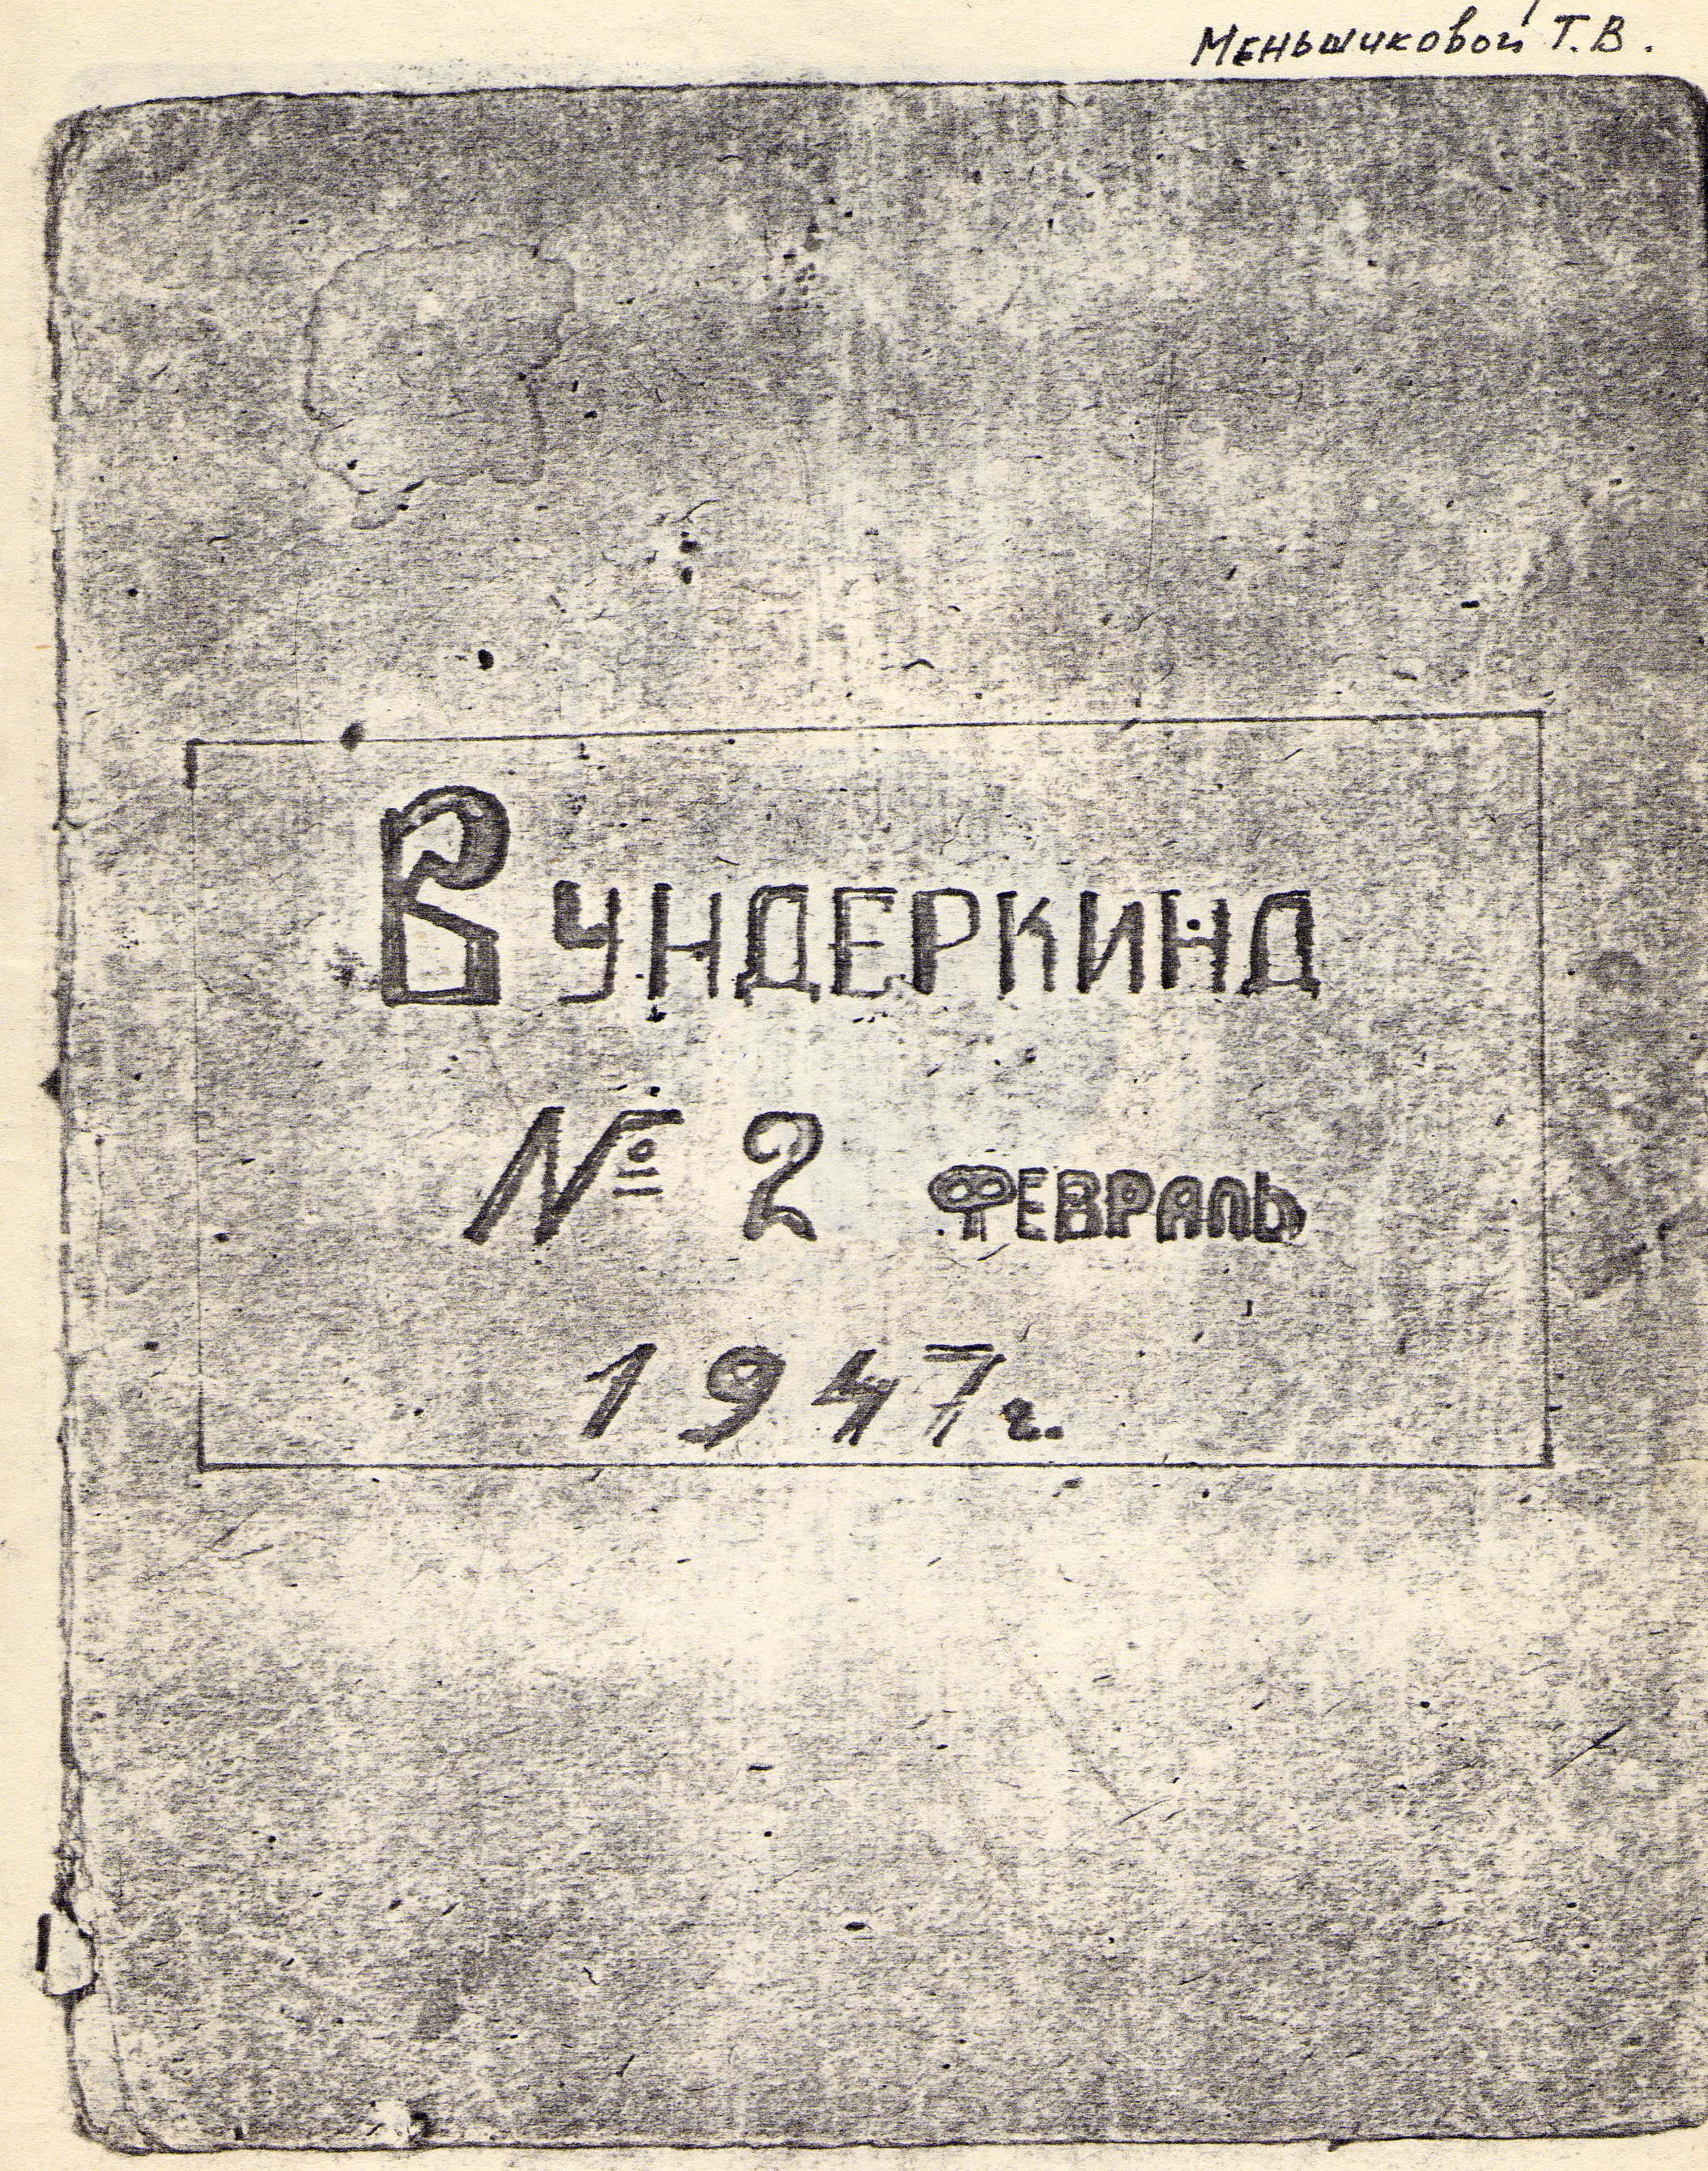
\includegraphics[width=\textwidth]{inc/Vynd/Vynd001}

\newpage

\noindent
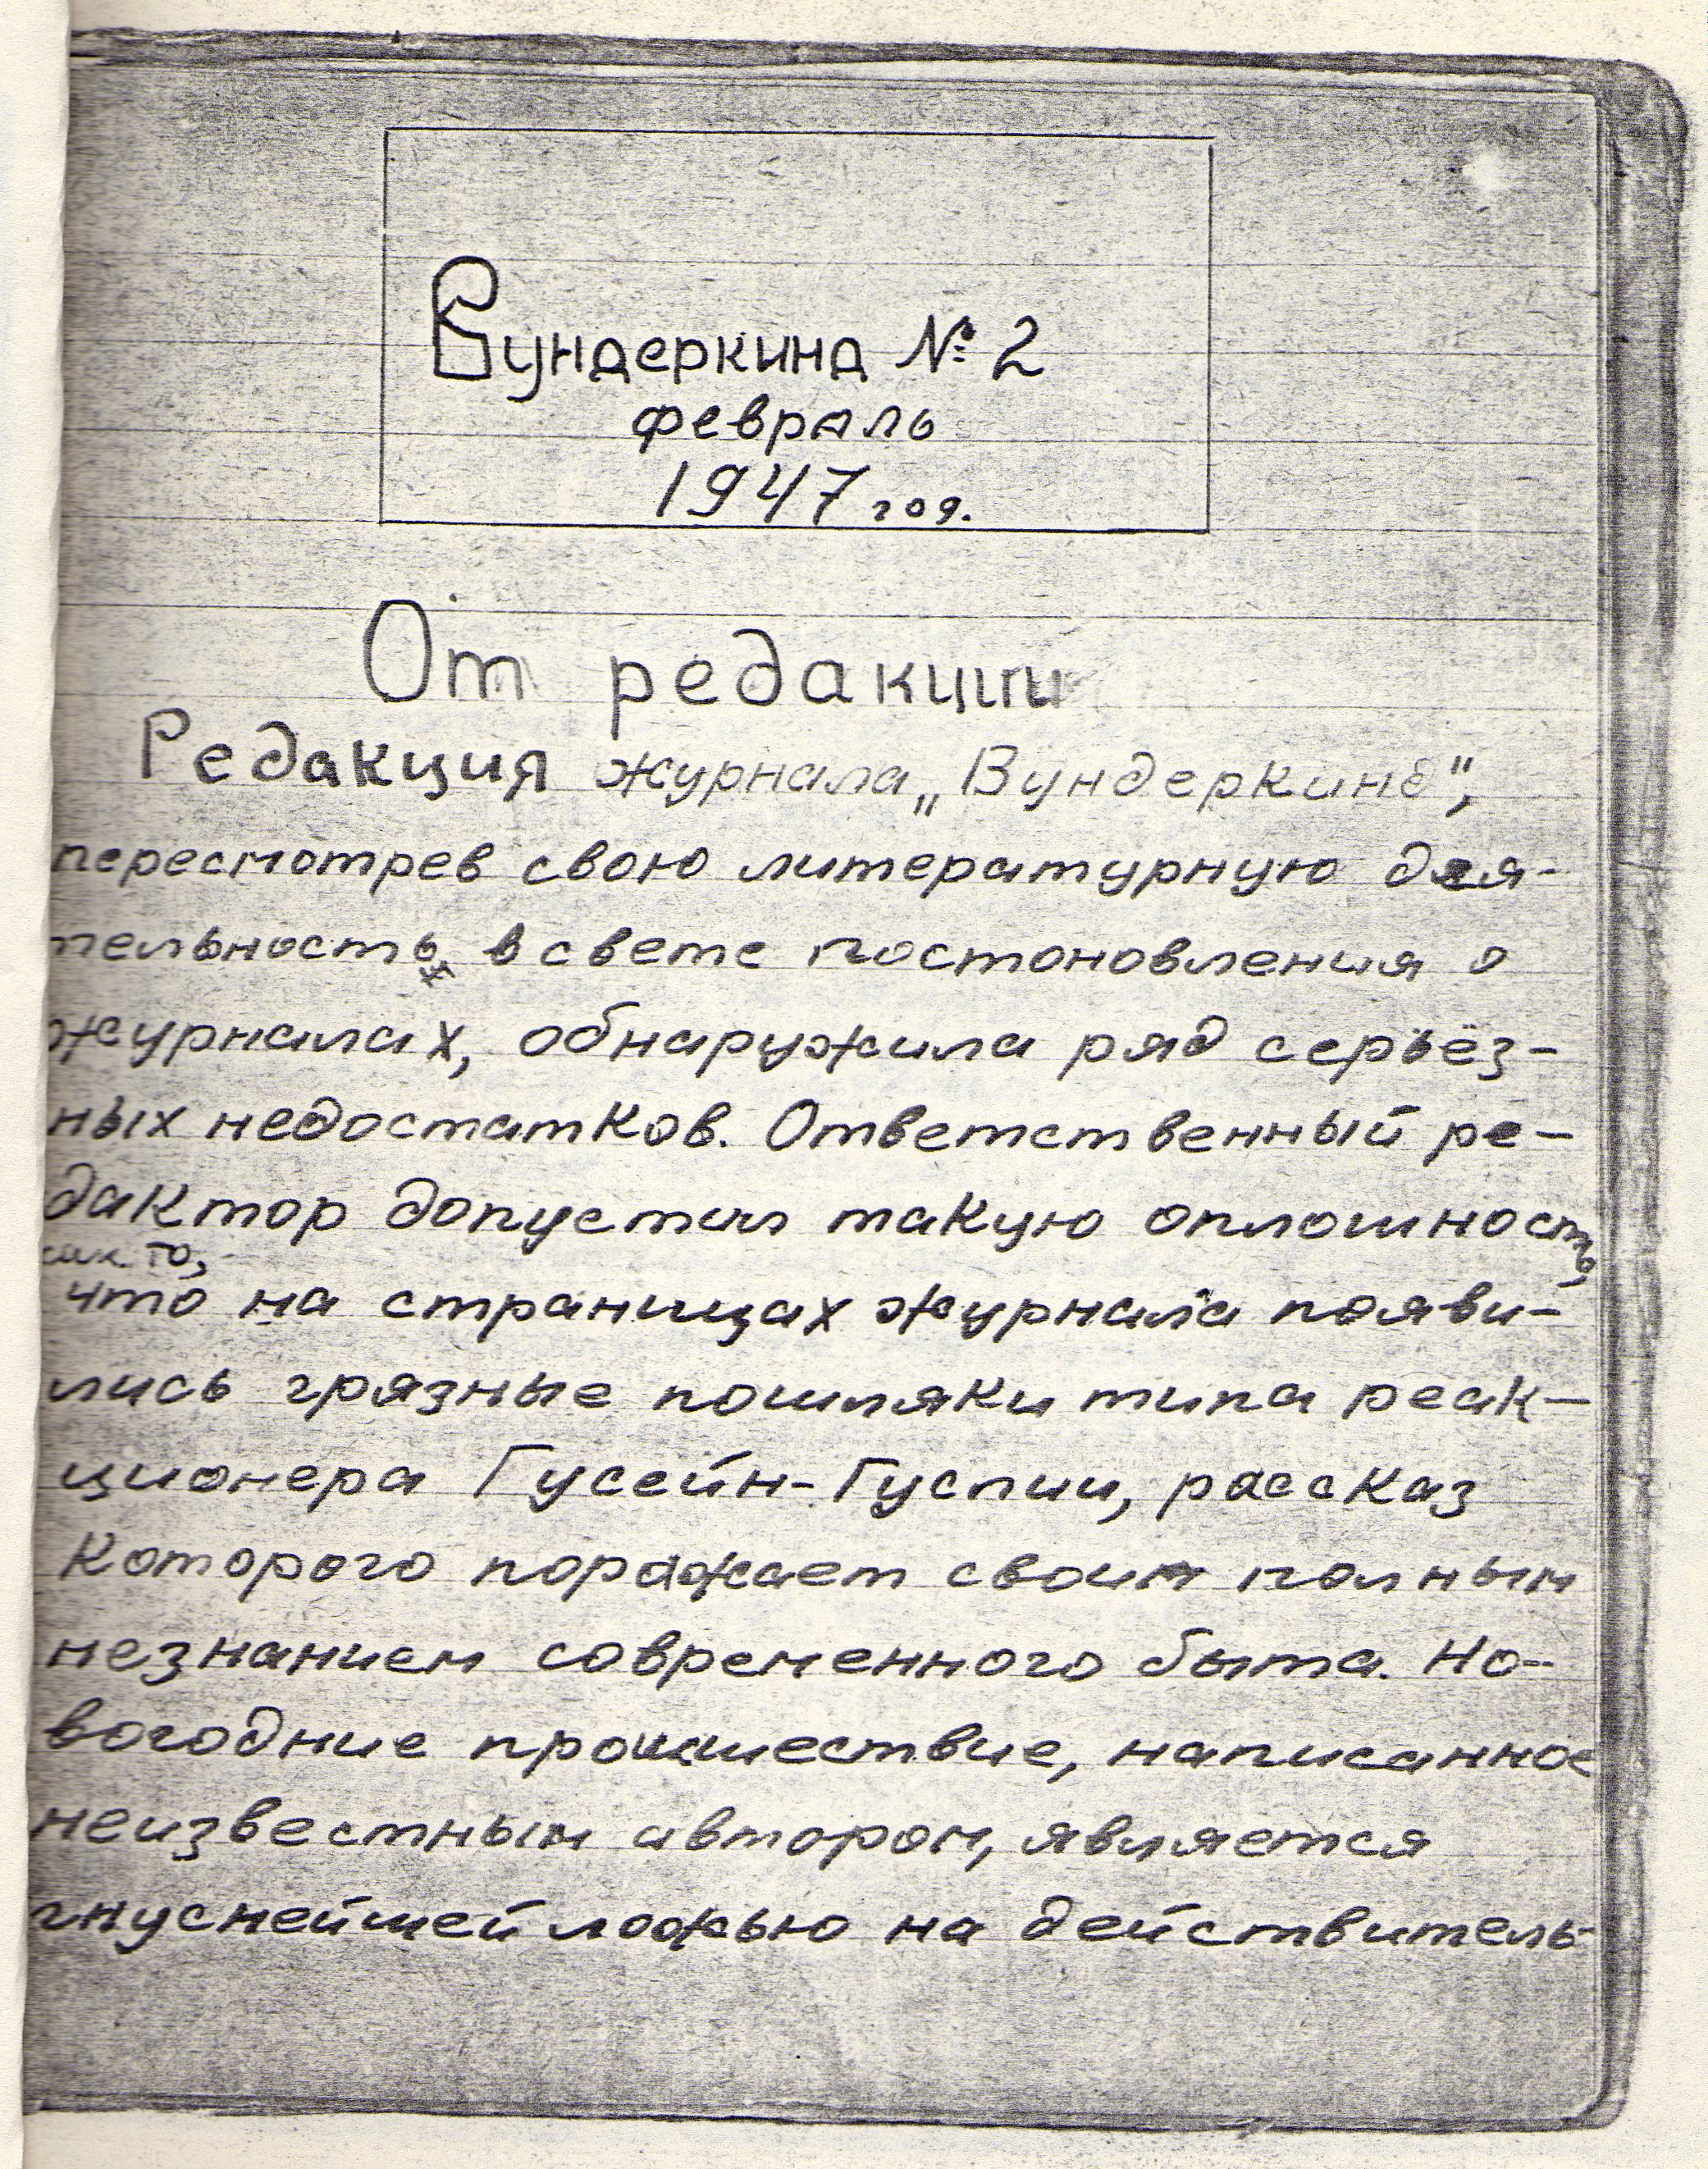
\includegraphics[width=\textwidth]{inc/Vynd/Vynd002}

\noindent
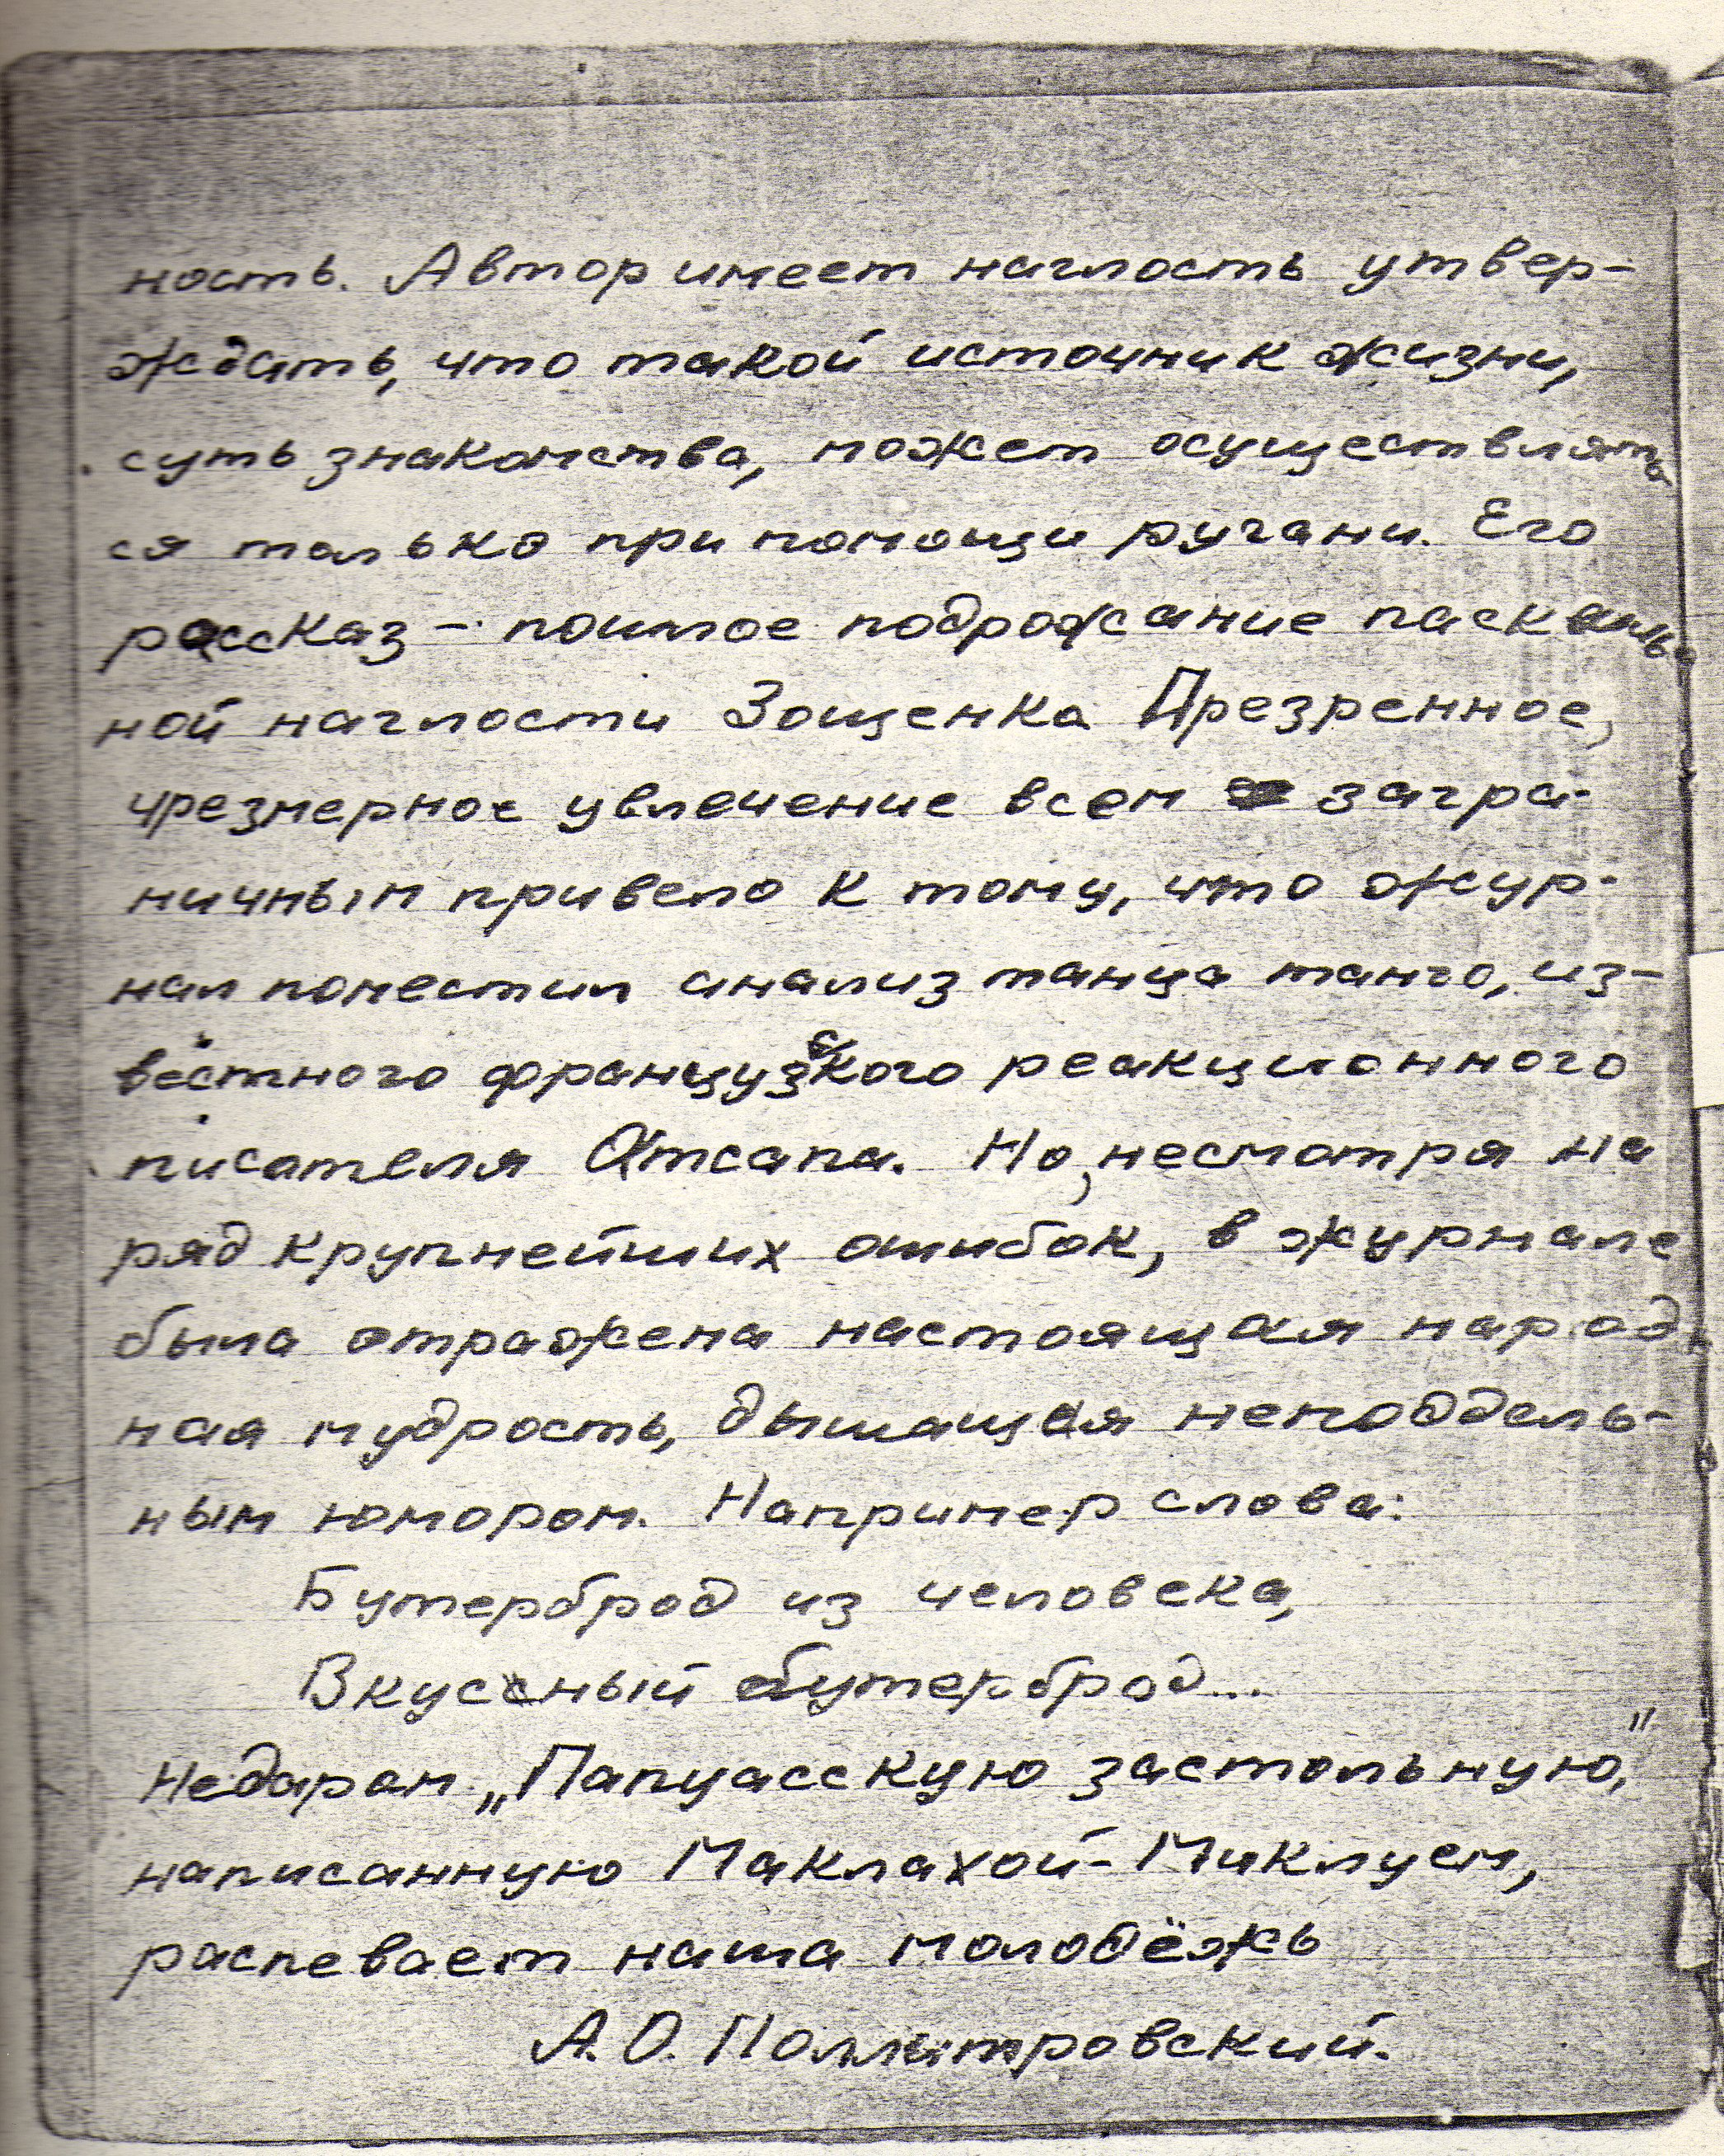
\includegraphics[width=\textwidth]{inc/Vynd/Vynd003}

\newpage


\noindent
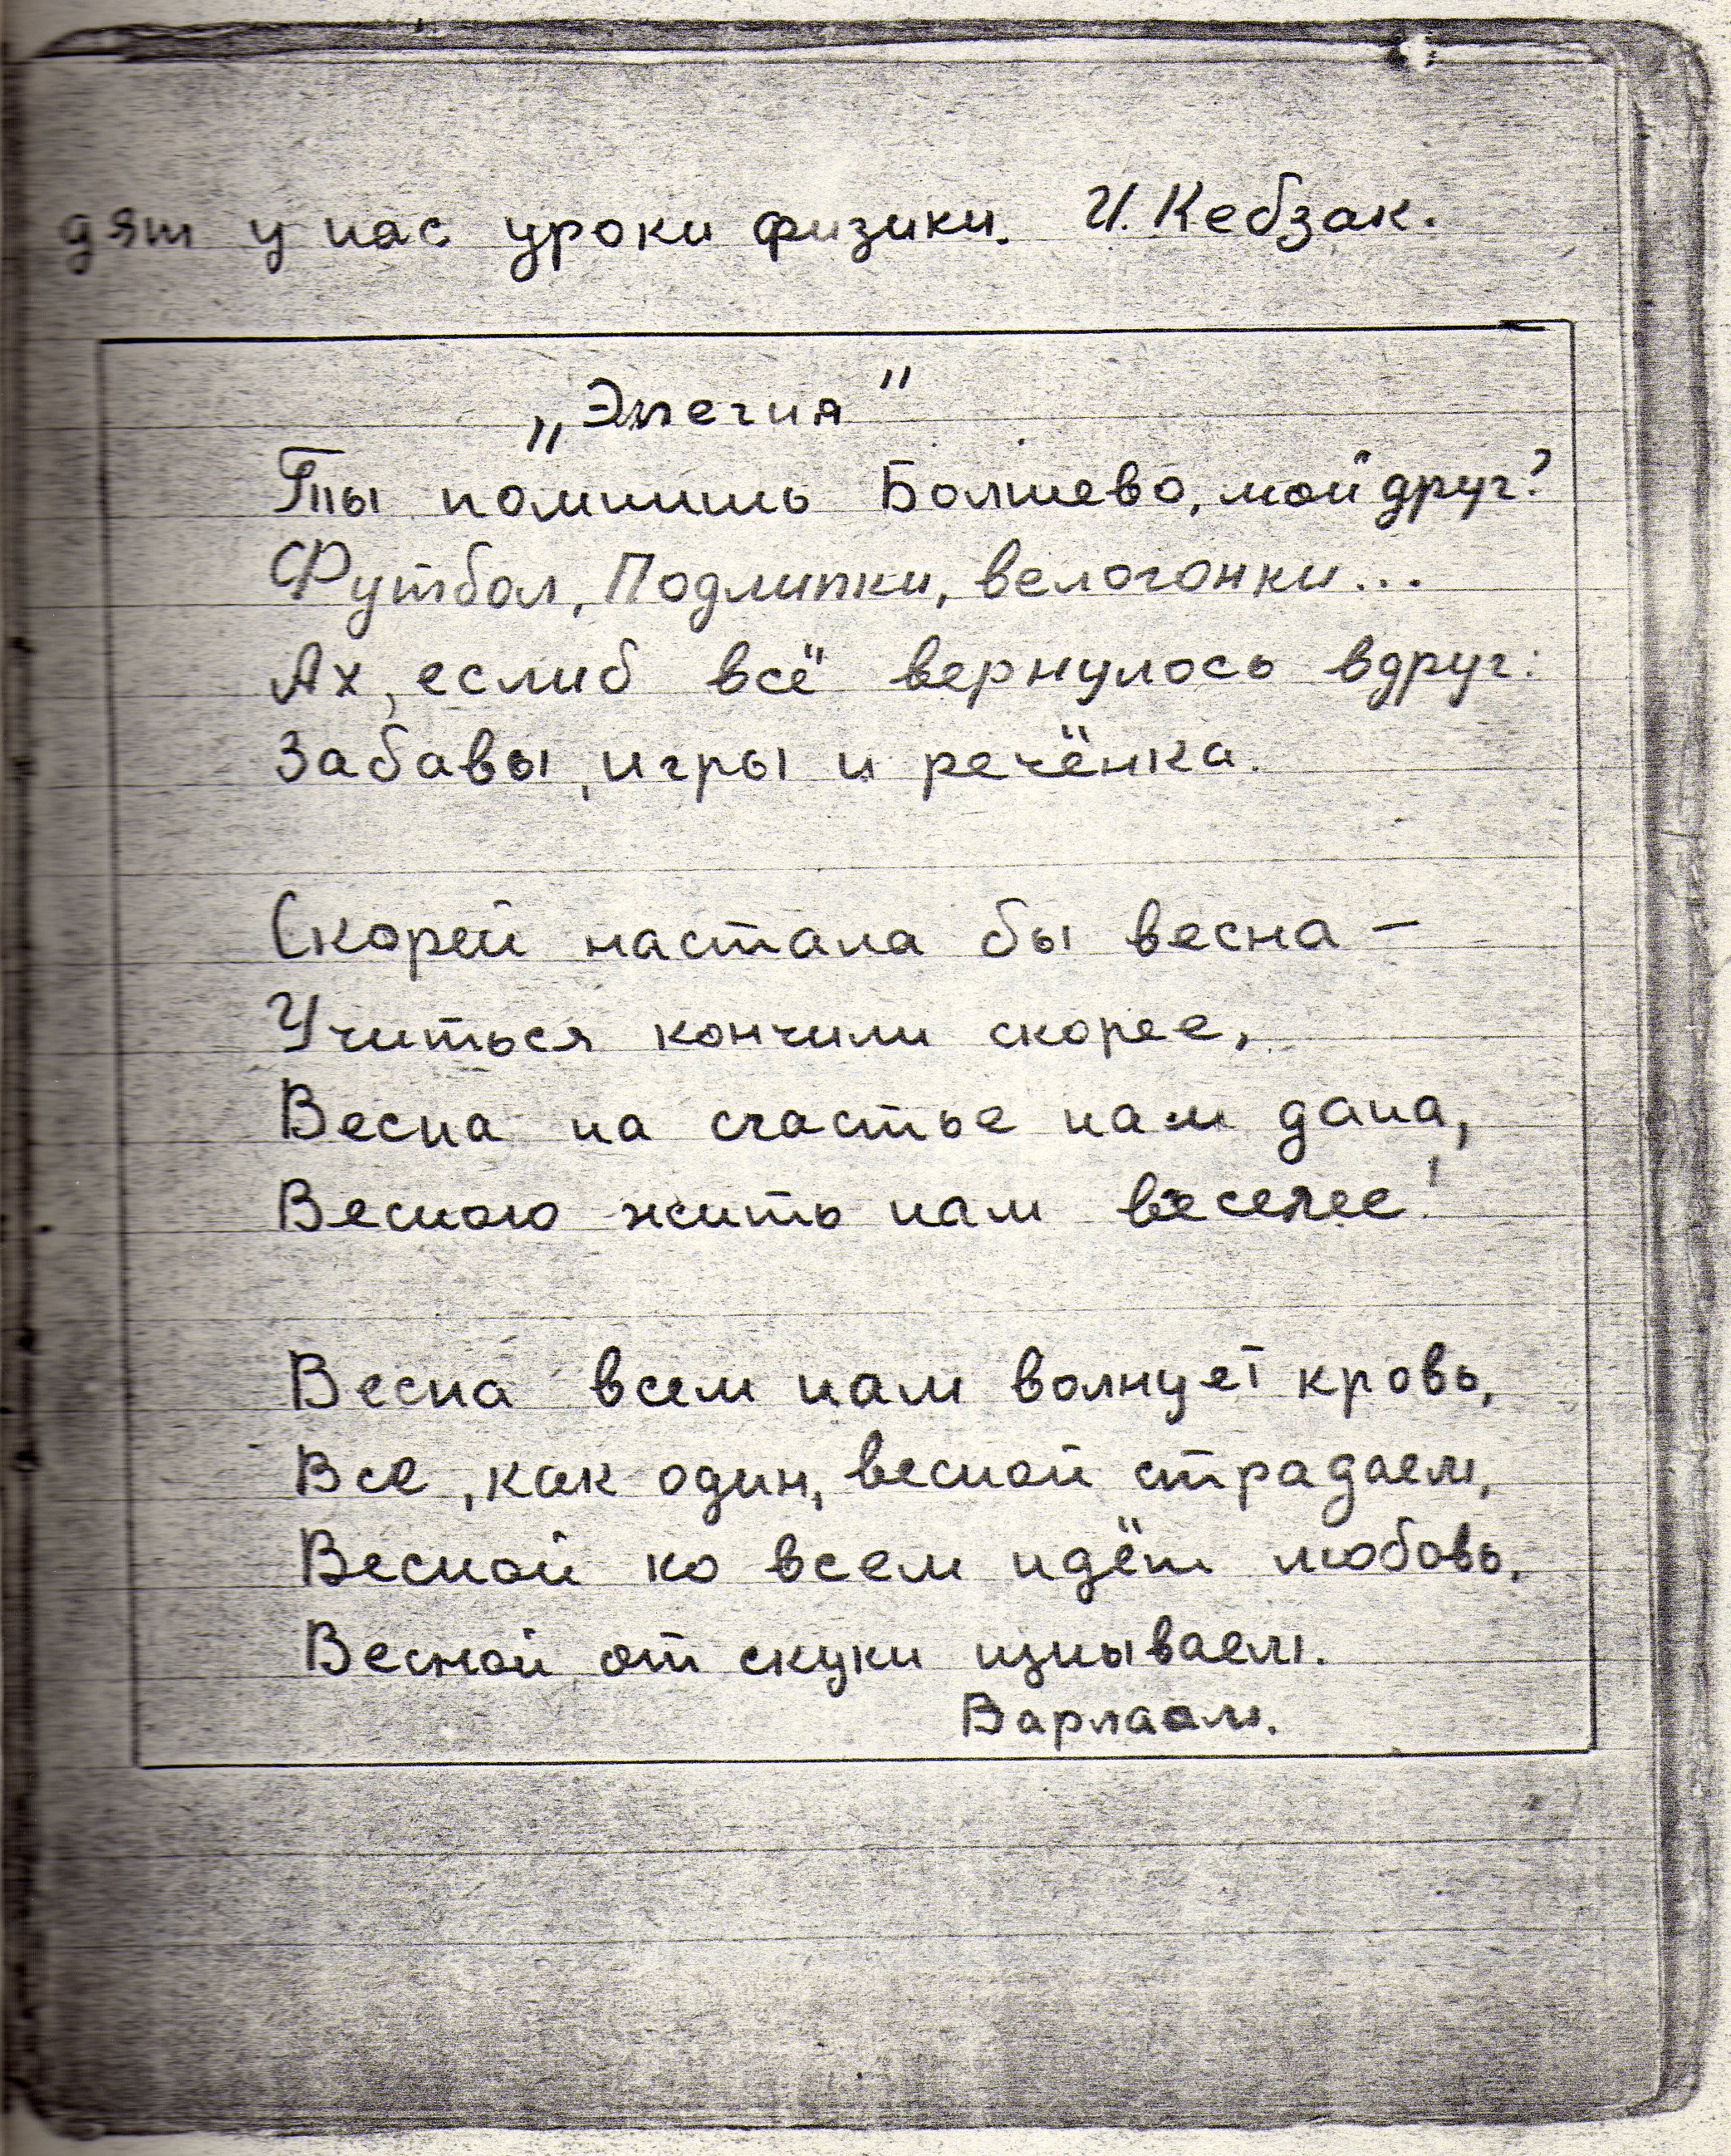
\includegraphics[width=\textwidth]{inc/Vynd/Vynd004}

\noindent
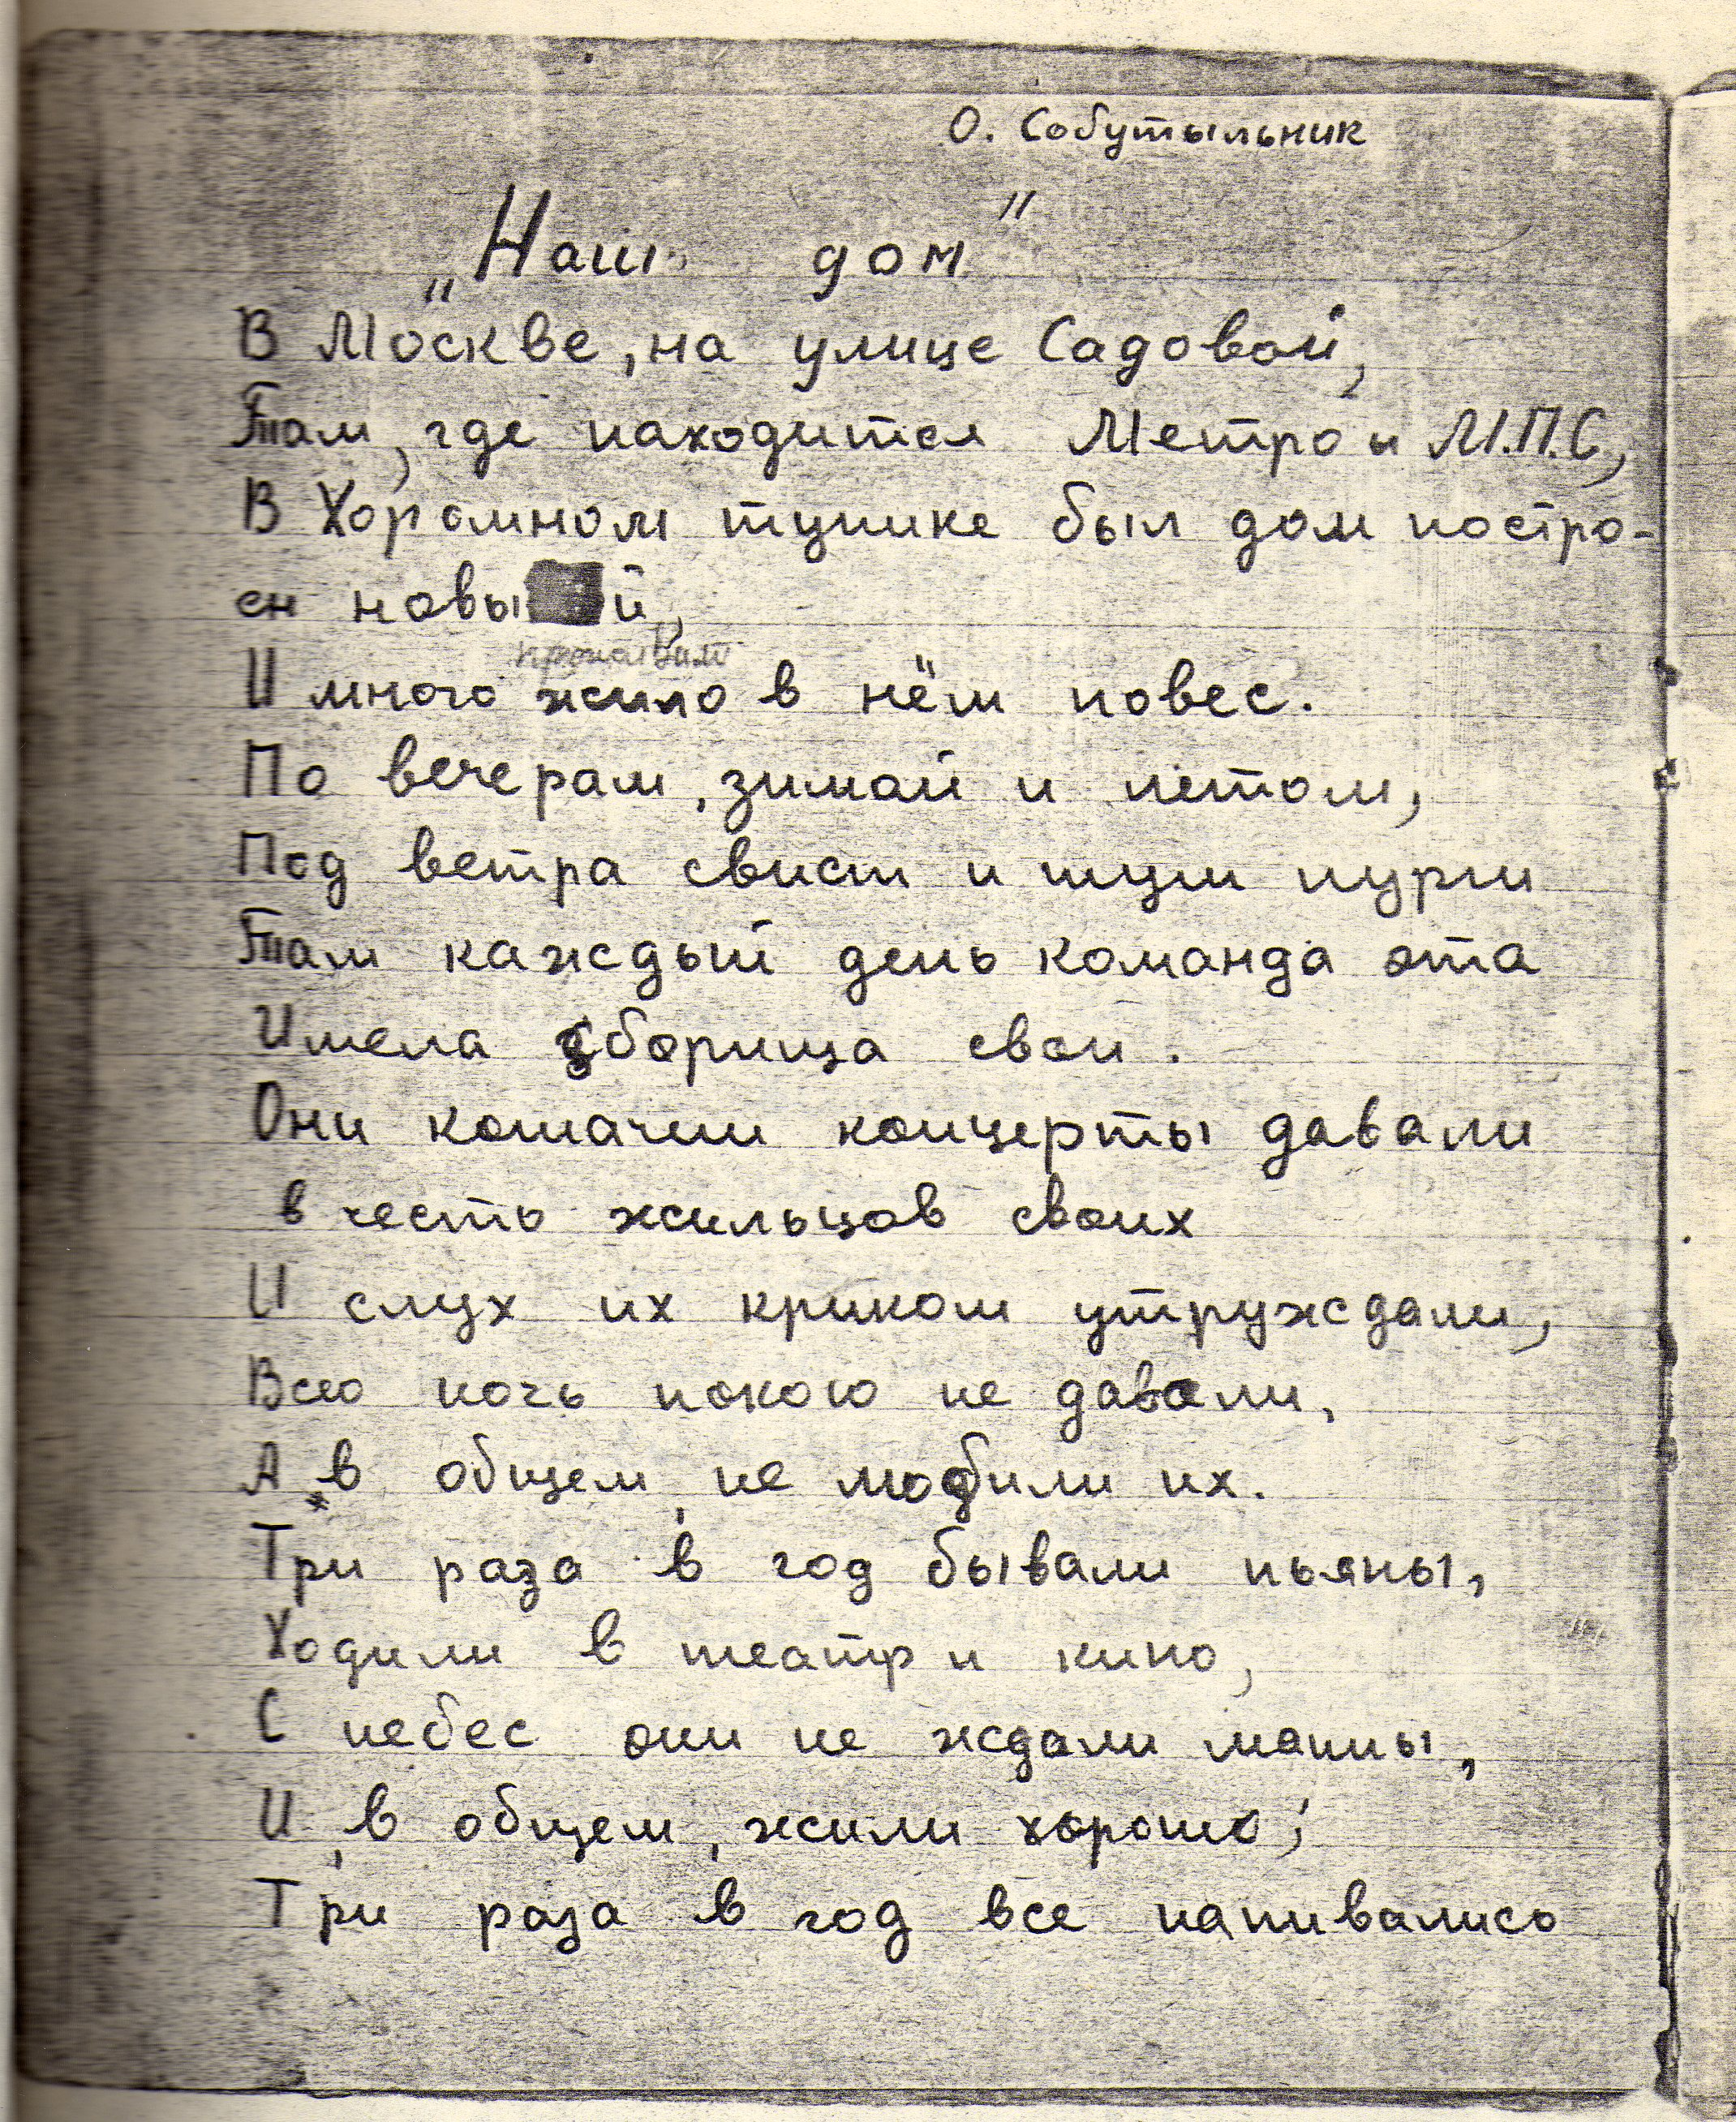
\includegraphics[width=\textwidth]{inc/Vynd/Vynd005}

\noindent
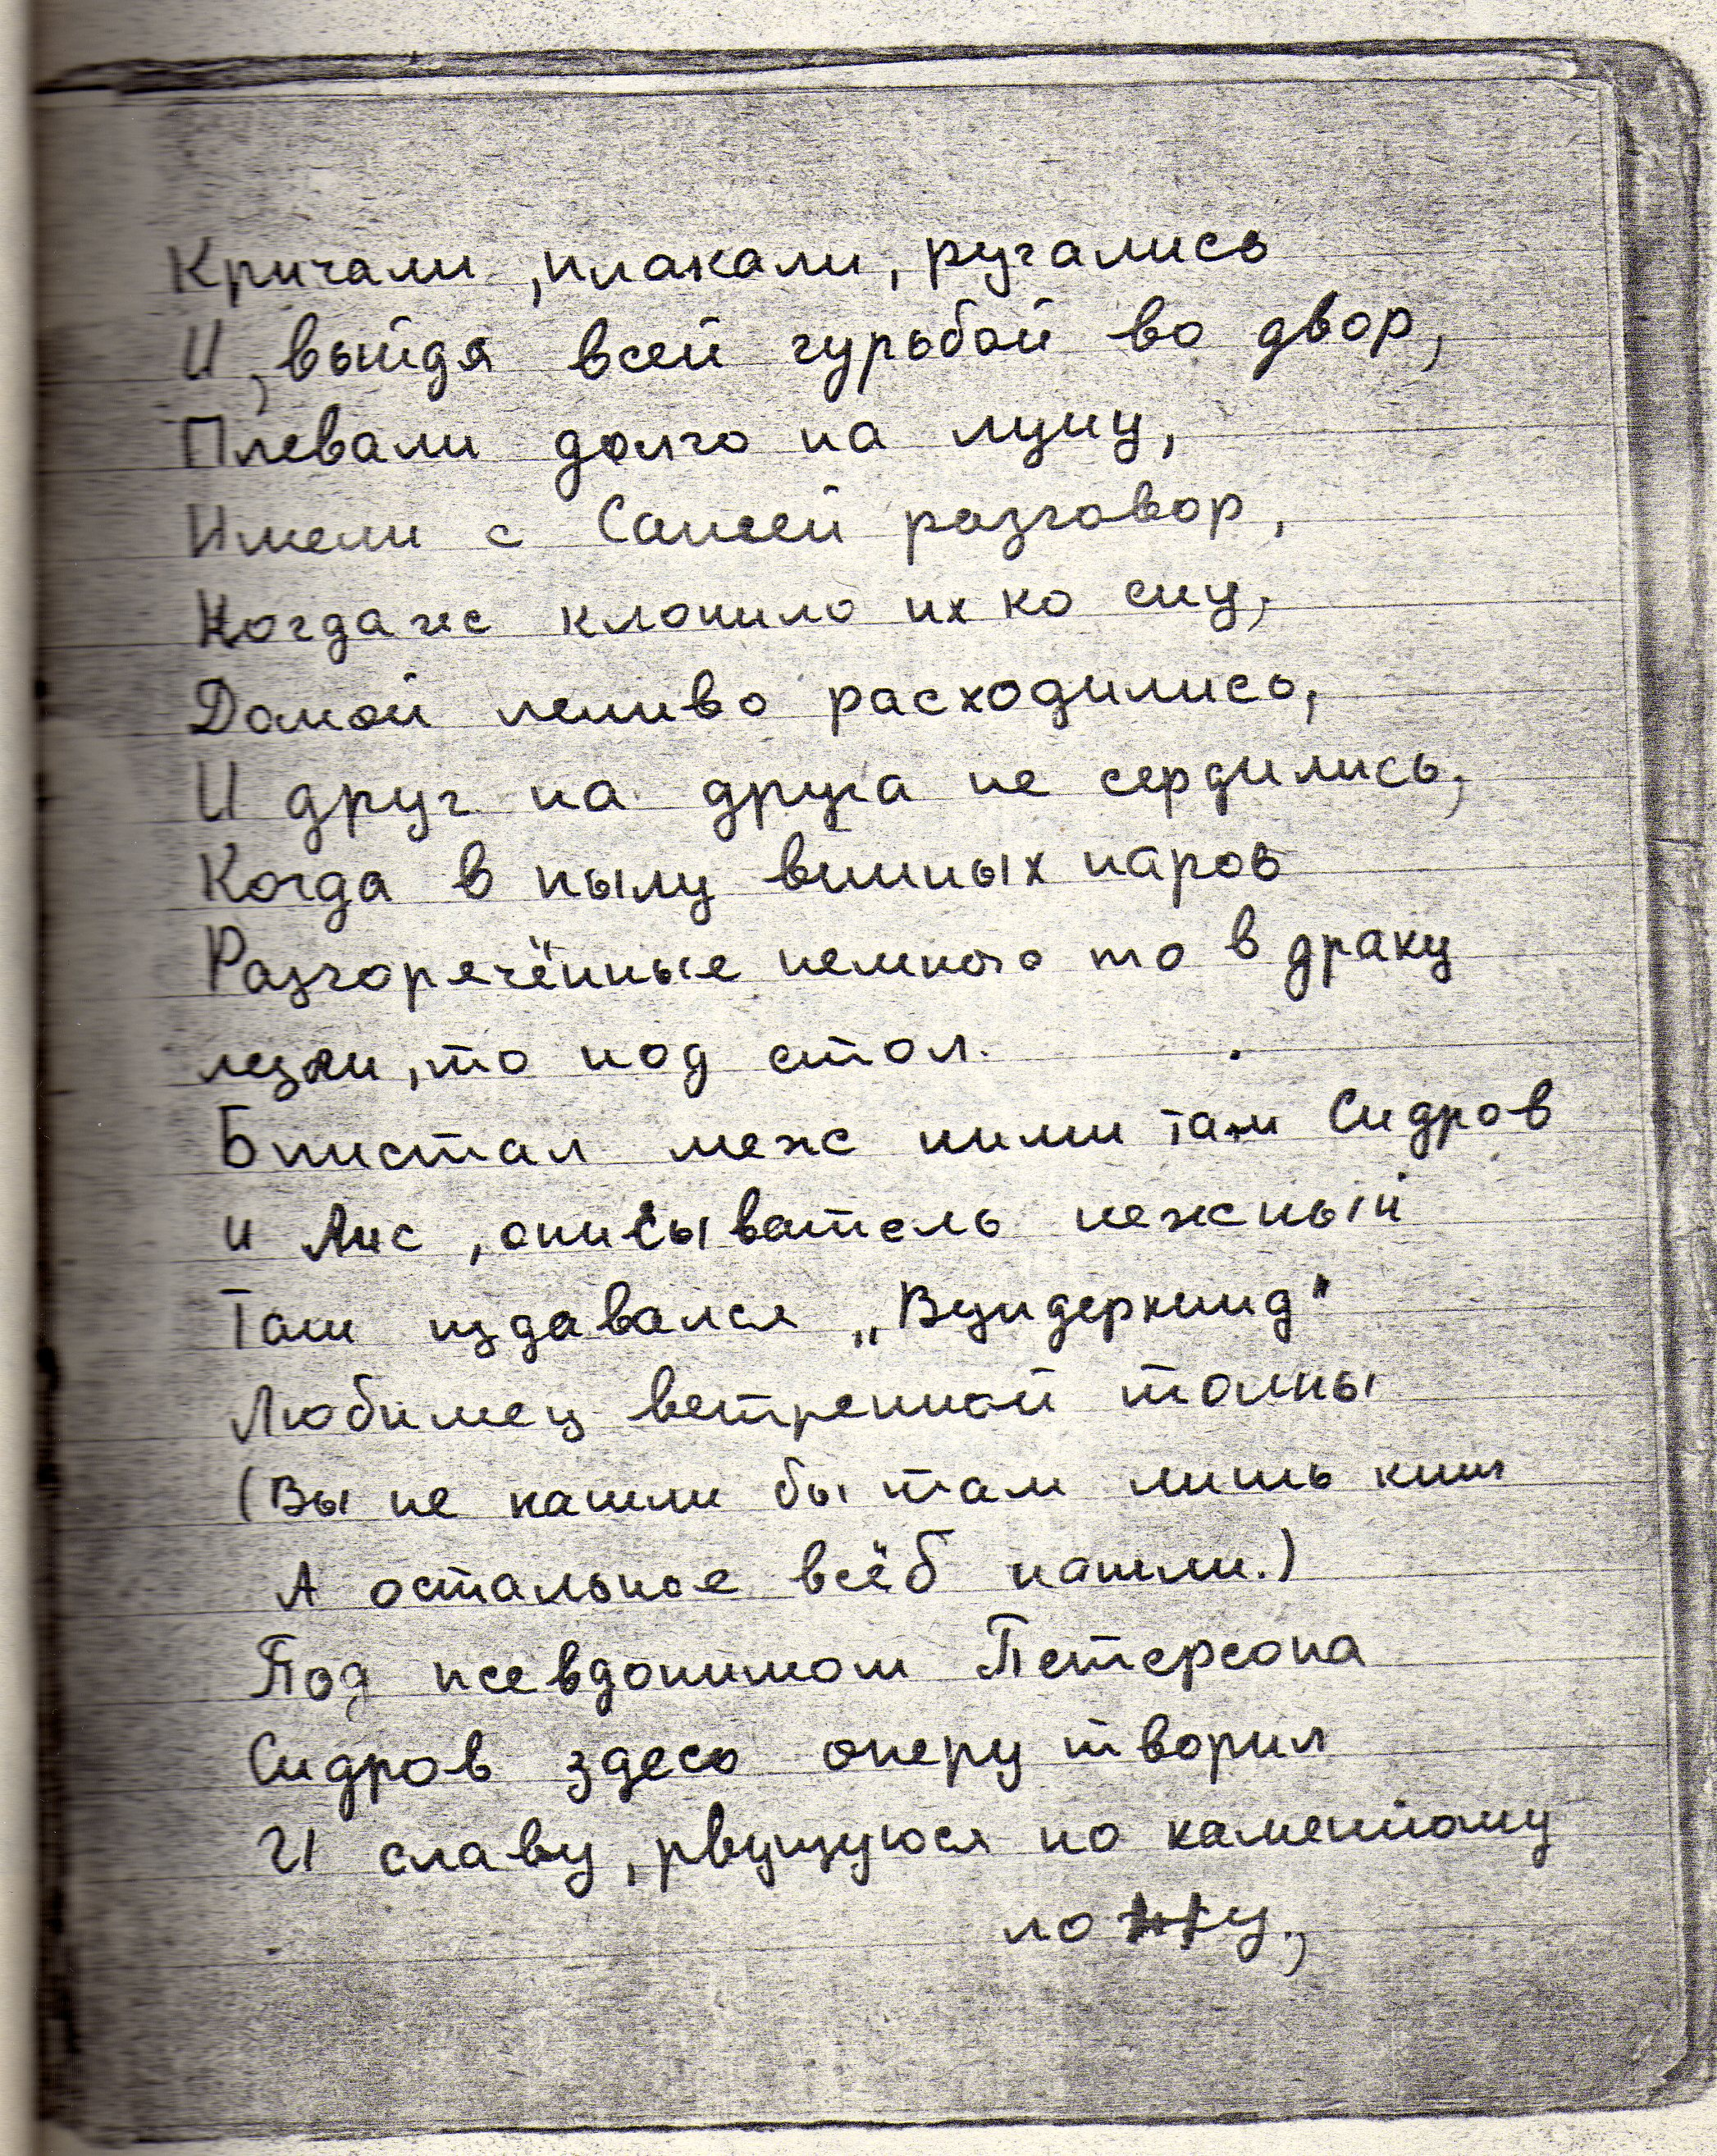
\includegraphics[width=\textwidth]{inc/Vynd/Vynd006}

\noindent
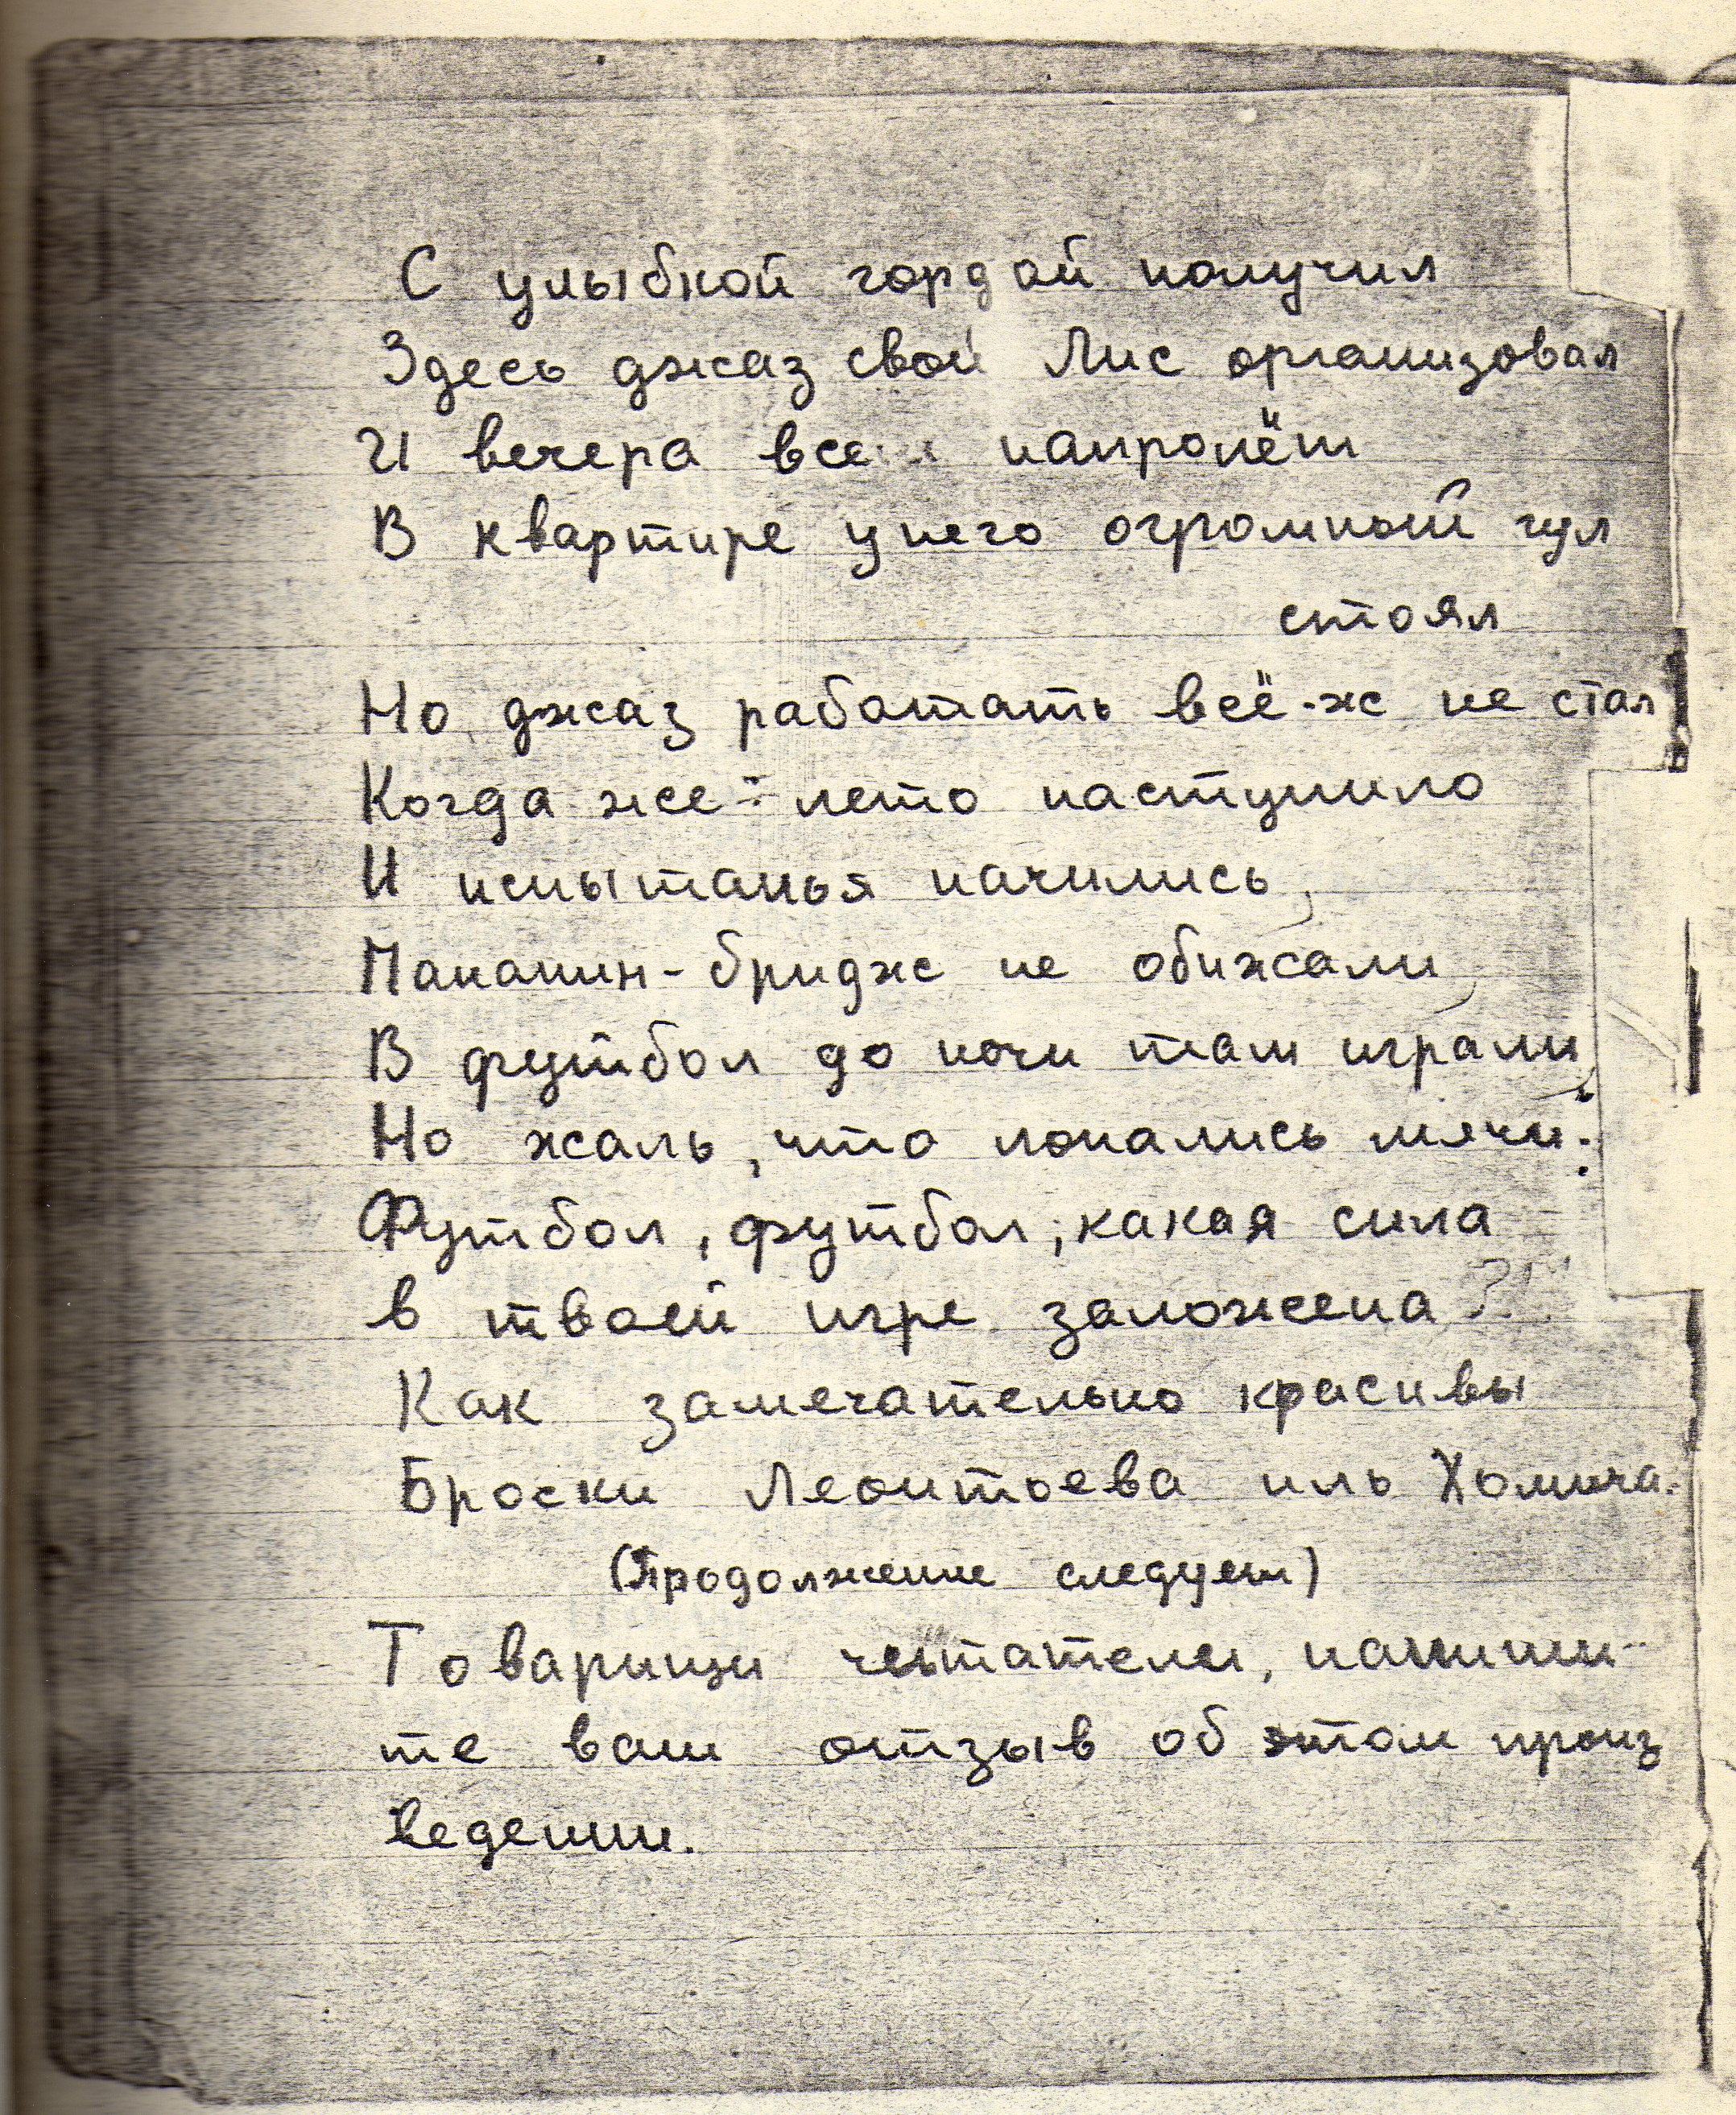
\includegraphics[width=\textwidth]{inc/Vynd/Vynd007}

\noindent
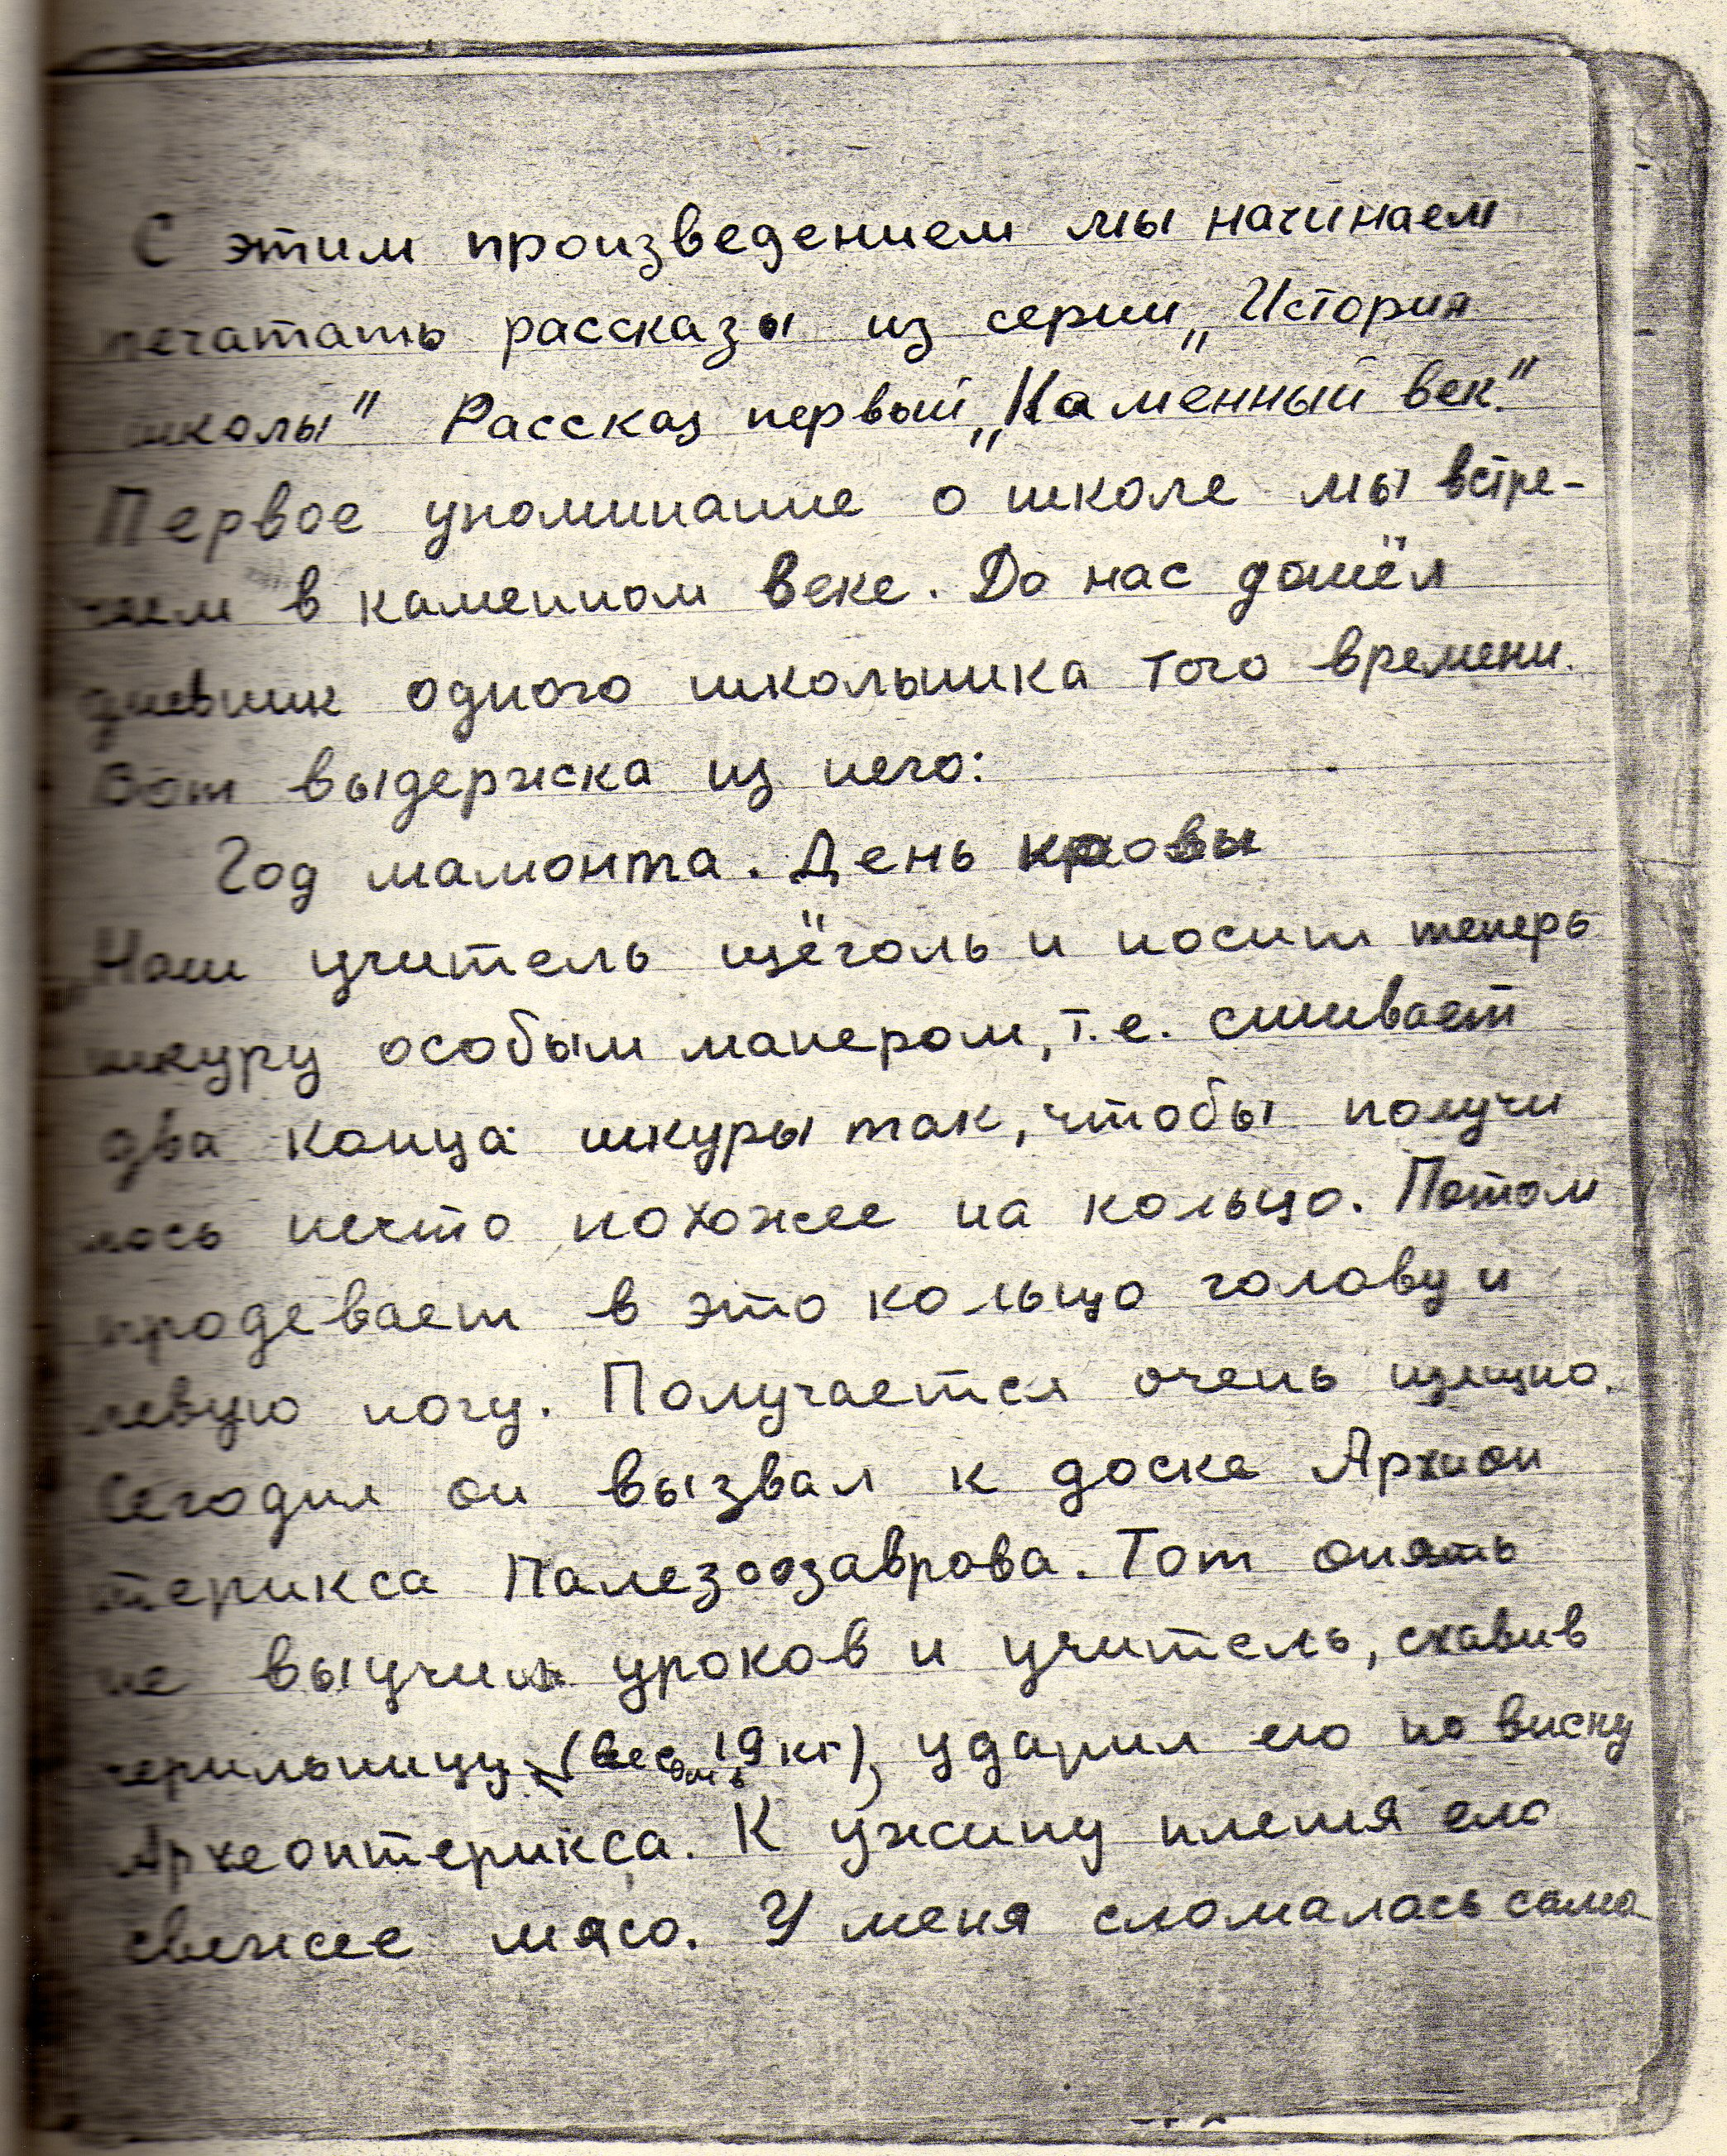
\includegraphics[width=\textwidth]{inc/Vynd/Vynd008}

\newpage

\noindent
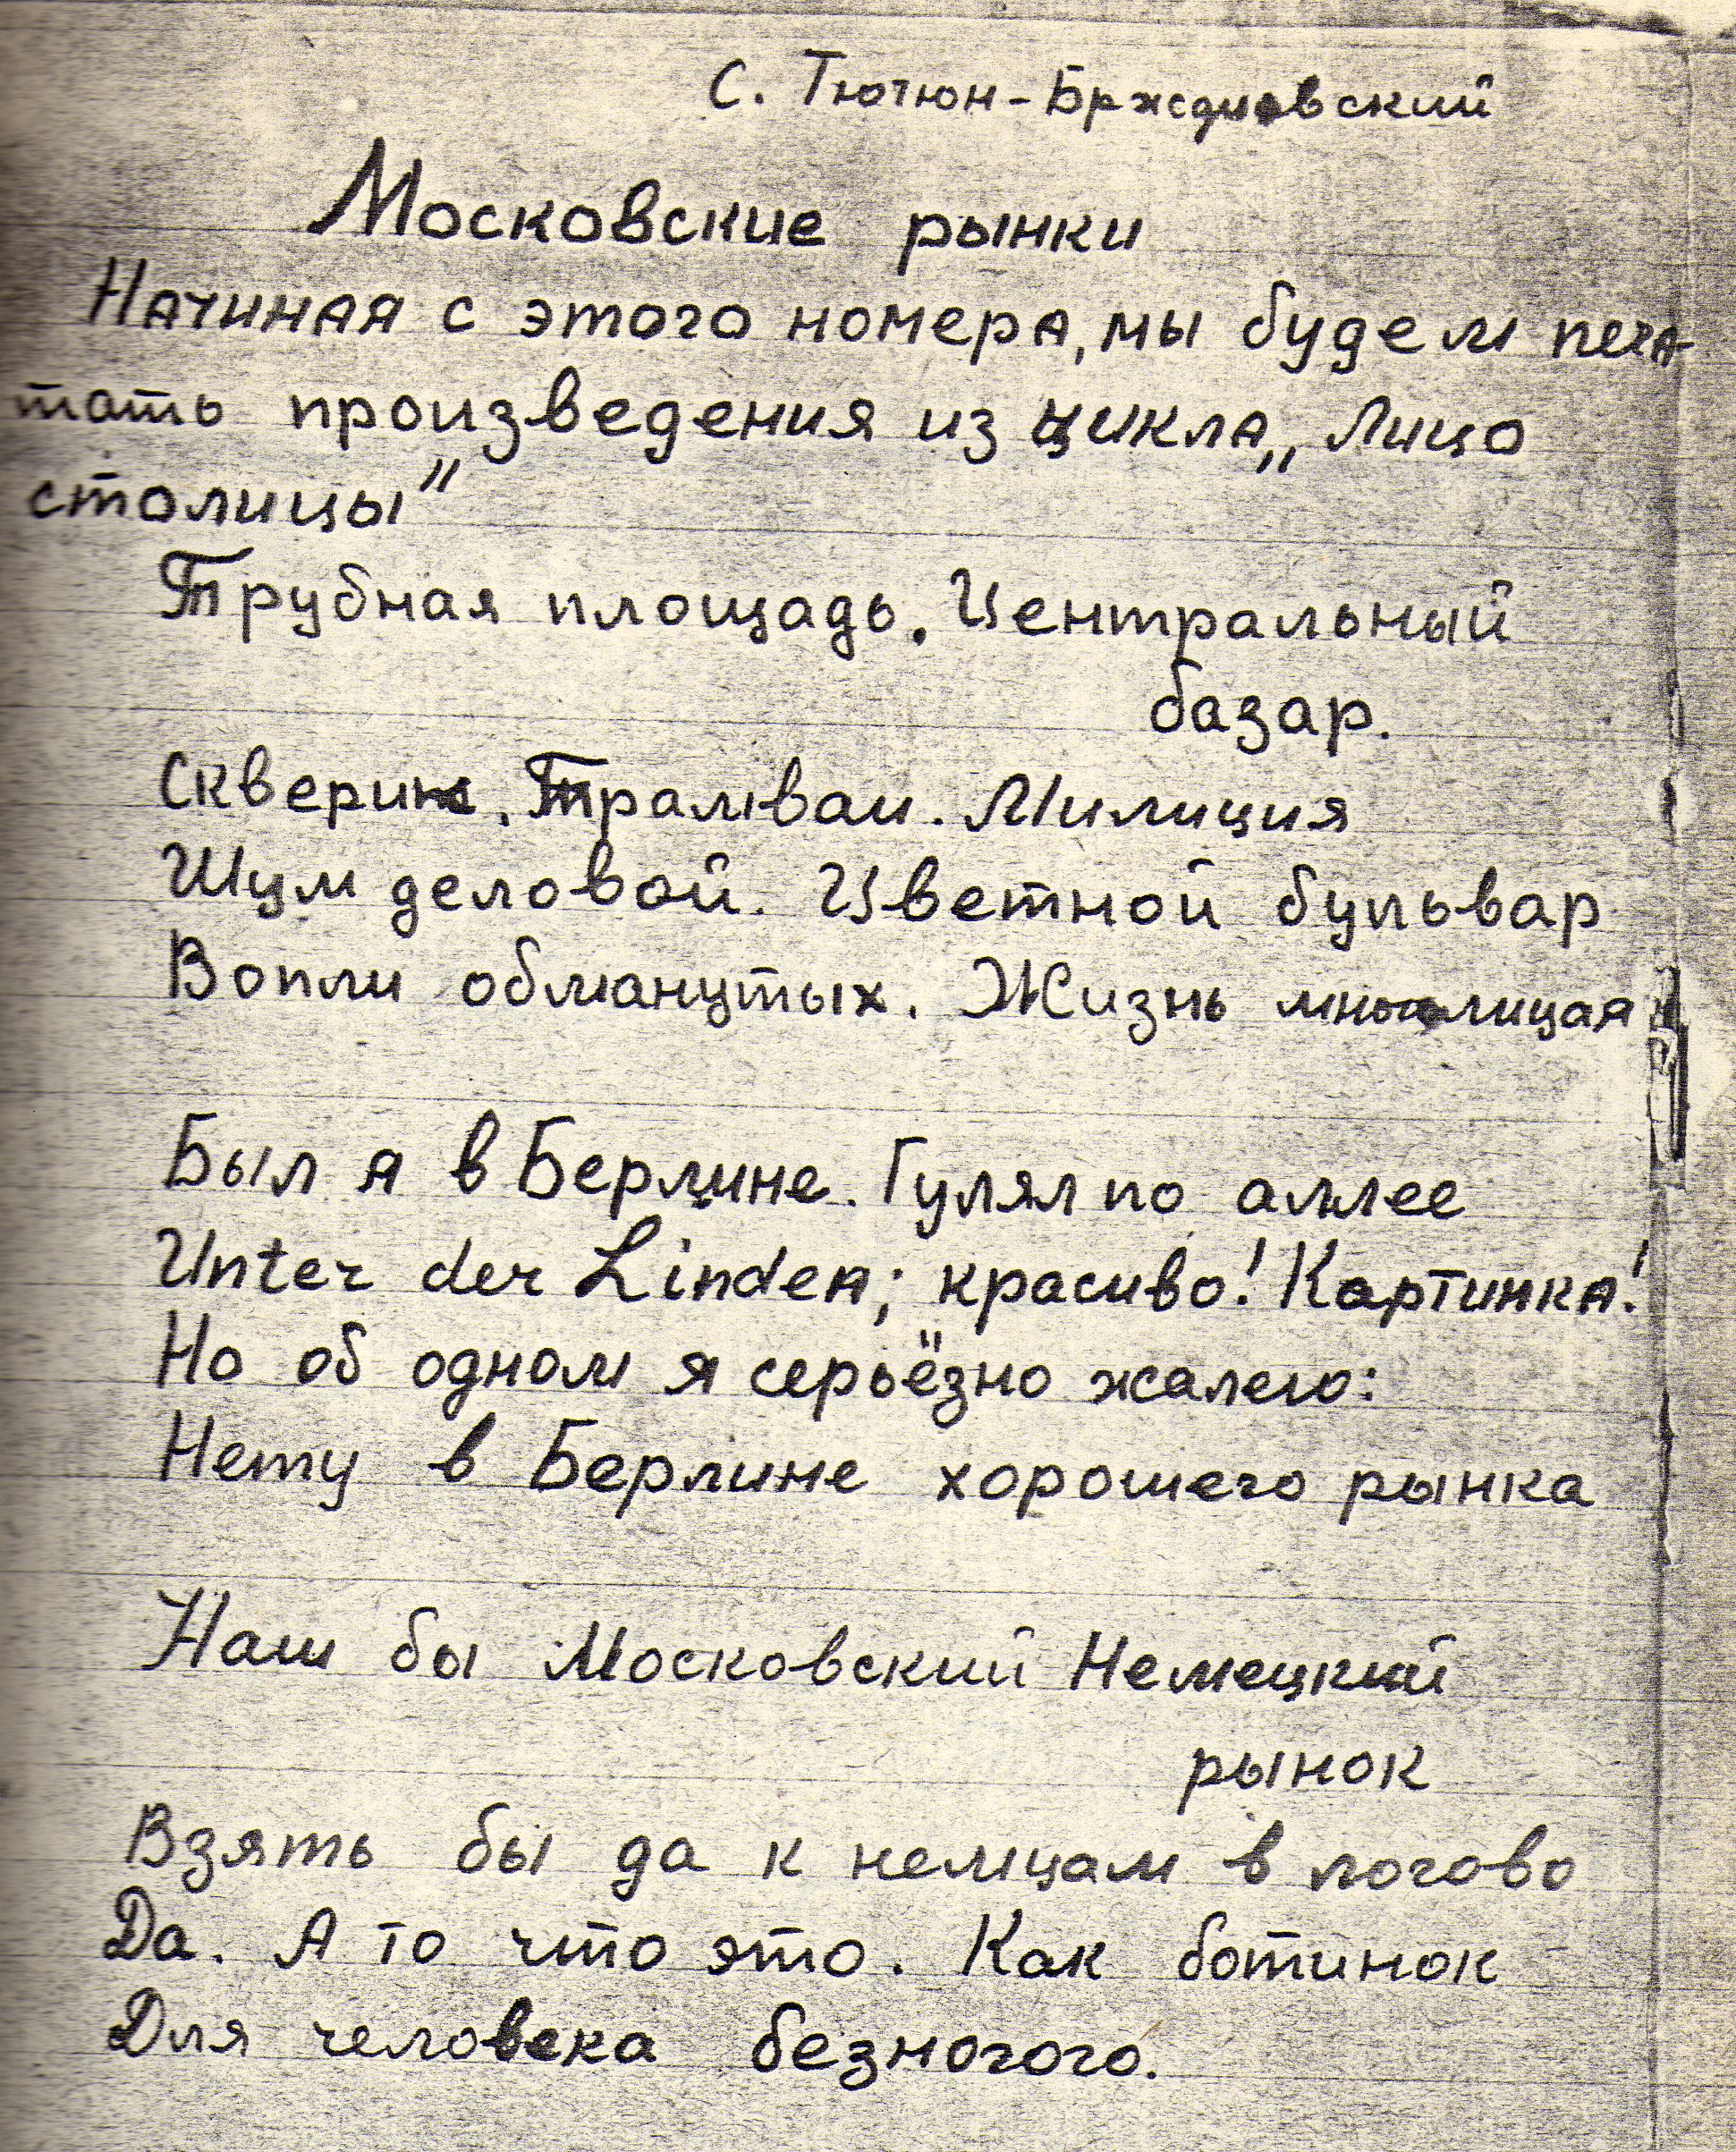
\includegraphics[width=\textwidth]{inc/Vynd/Vynd009}

\noindent
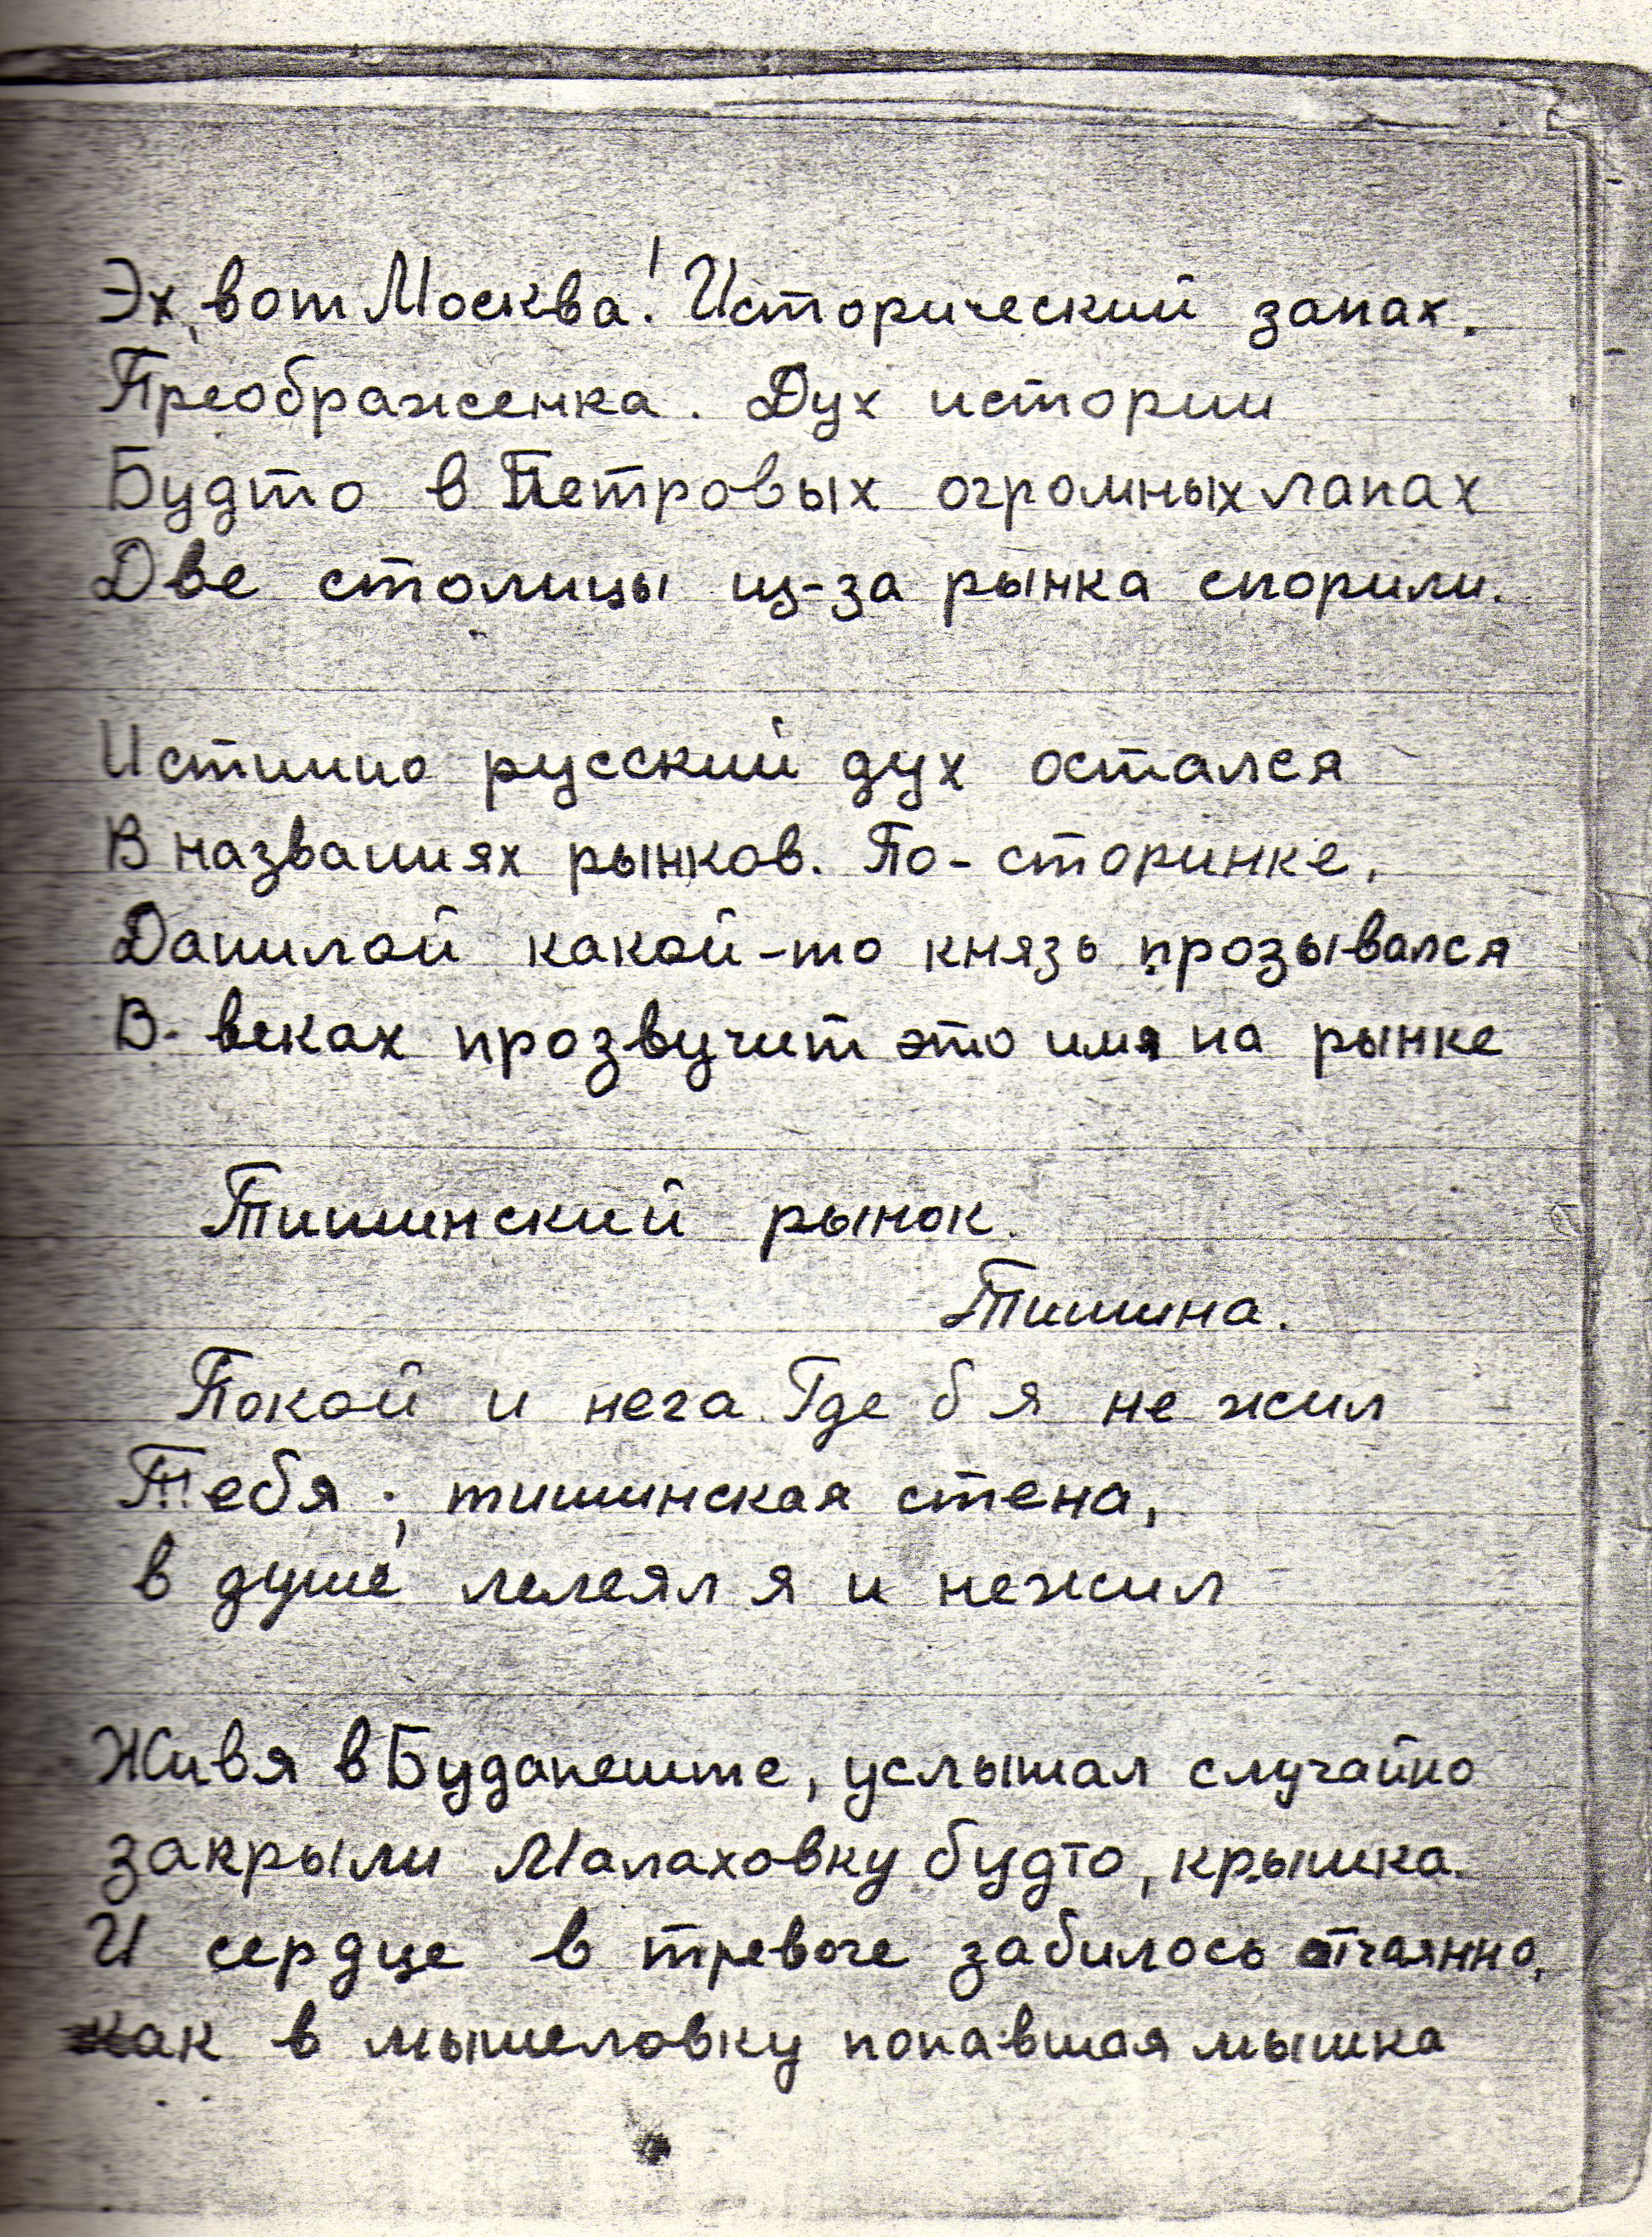
\includegraphics[width=\textwidth]{inc/Vynd/Vynd010}

\noindent
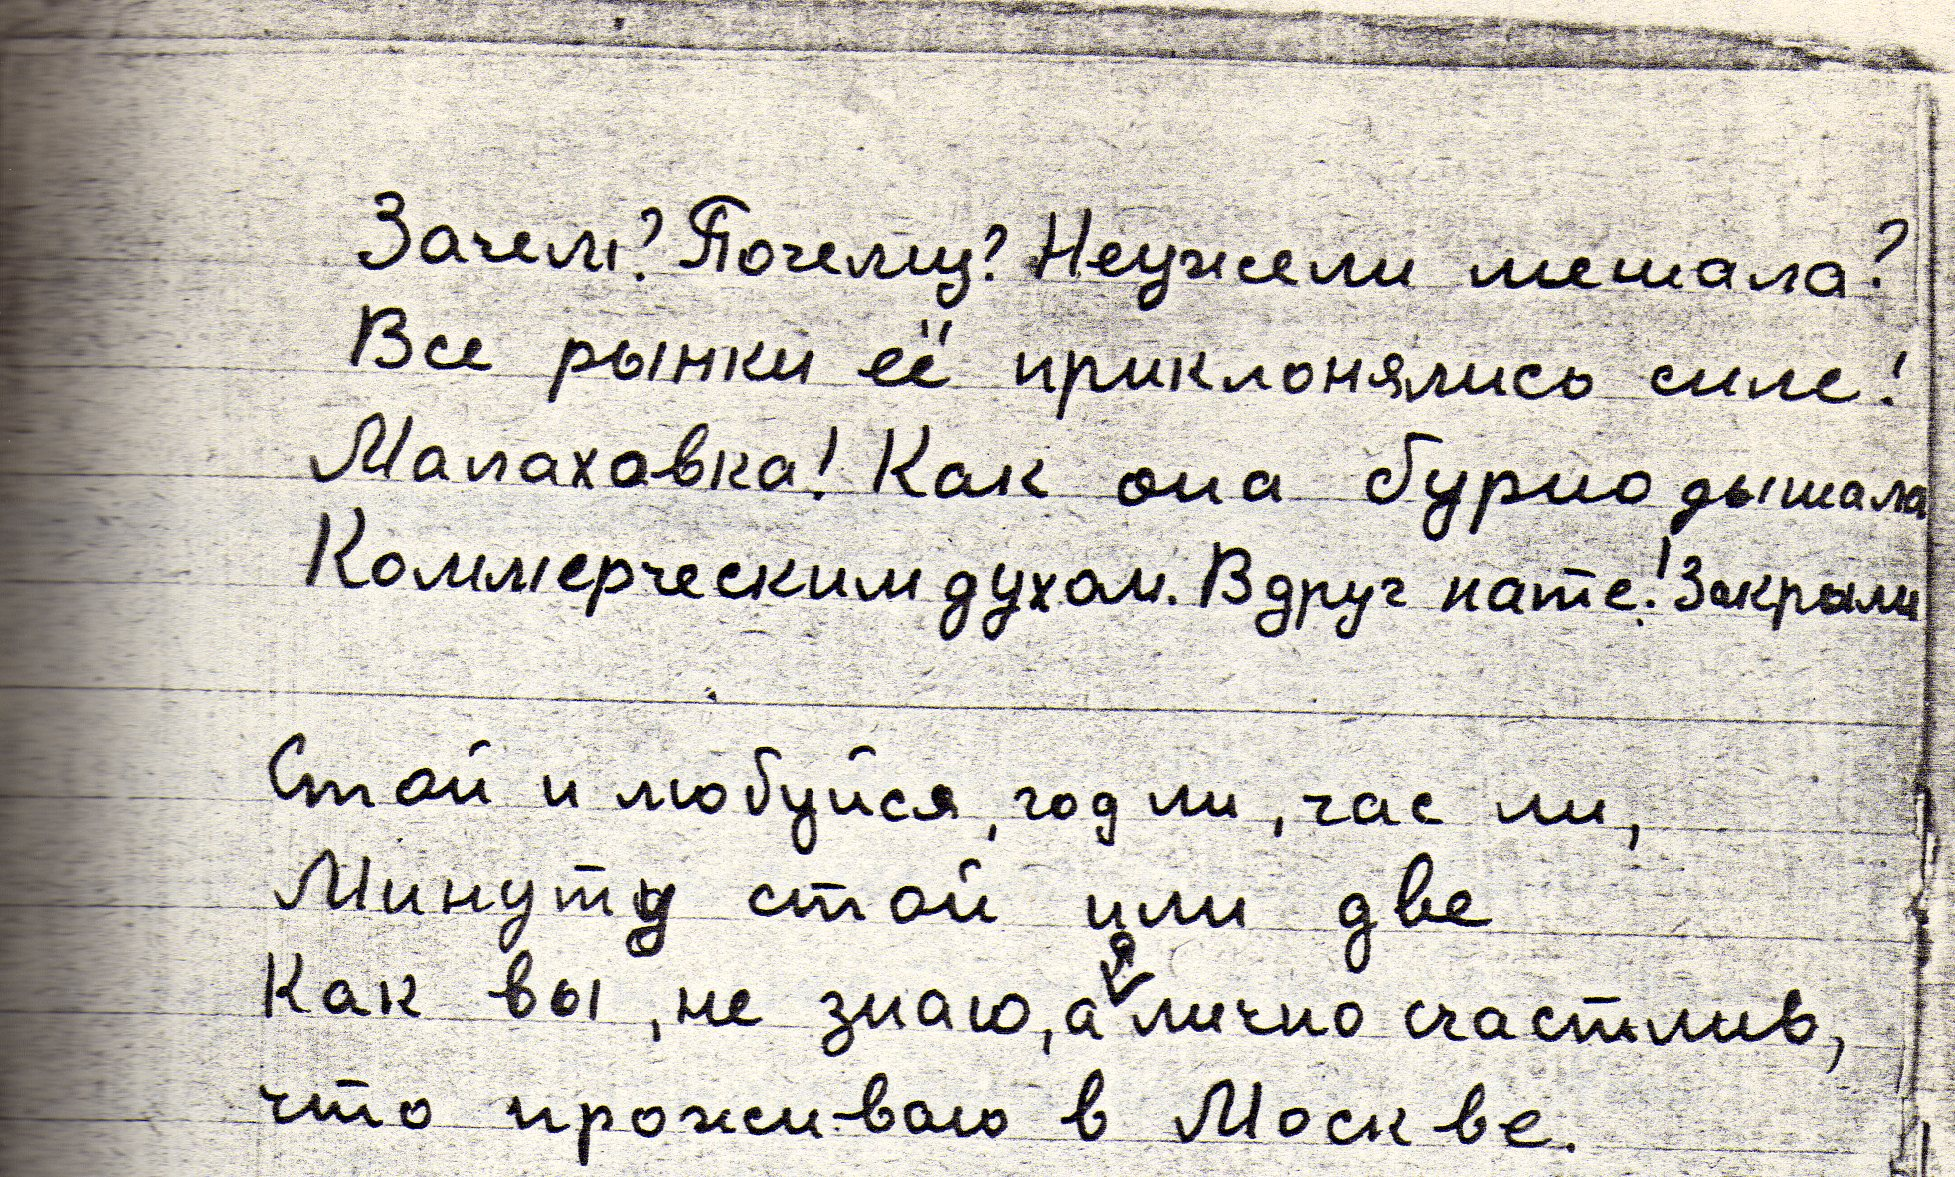
\includegraphics[width=\textwidth]{inc/Vynd/Vynd011}

\newpage


\noindent
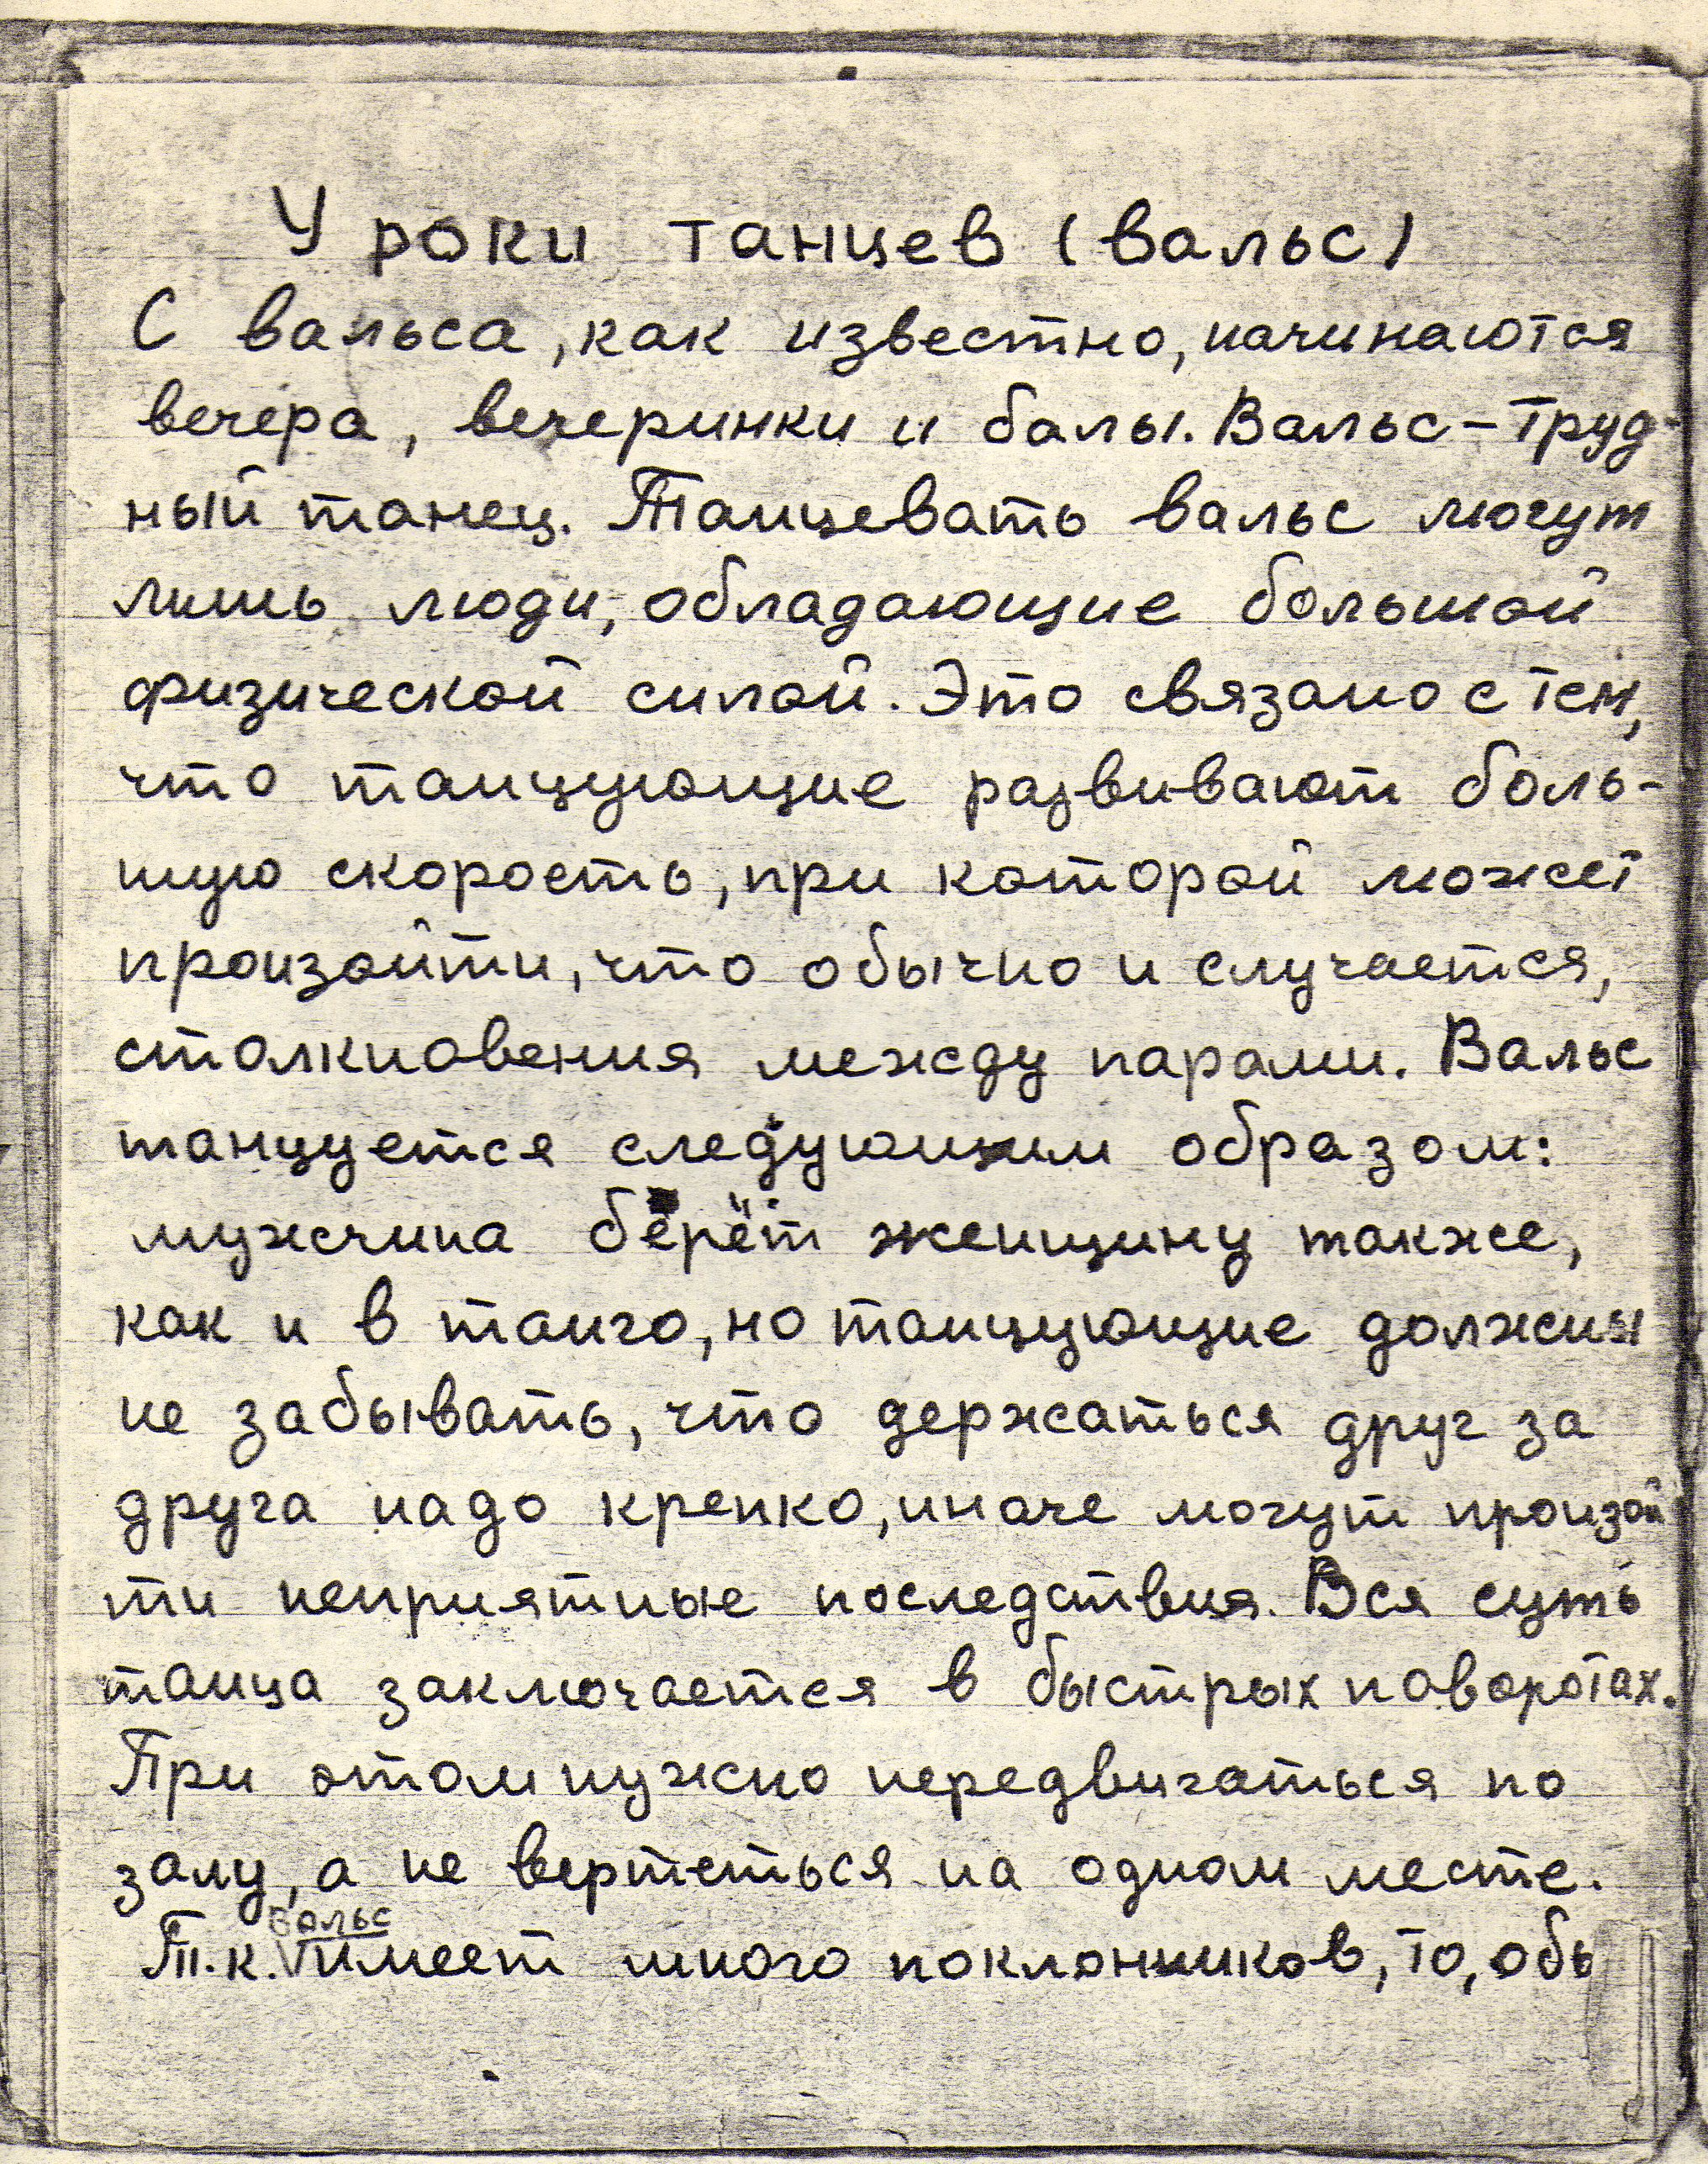
\includegraphics[width=\textwidth]{inc/Vynd/Vynd012}

\newpage

\noindent
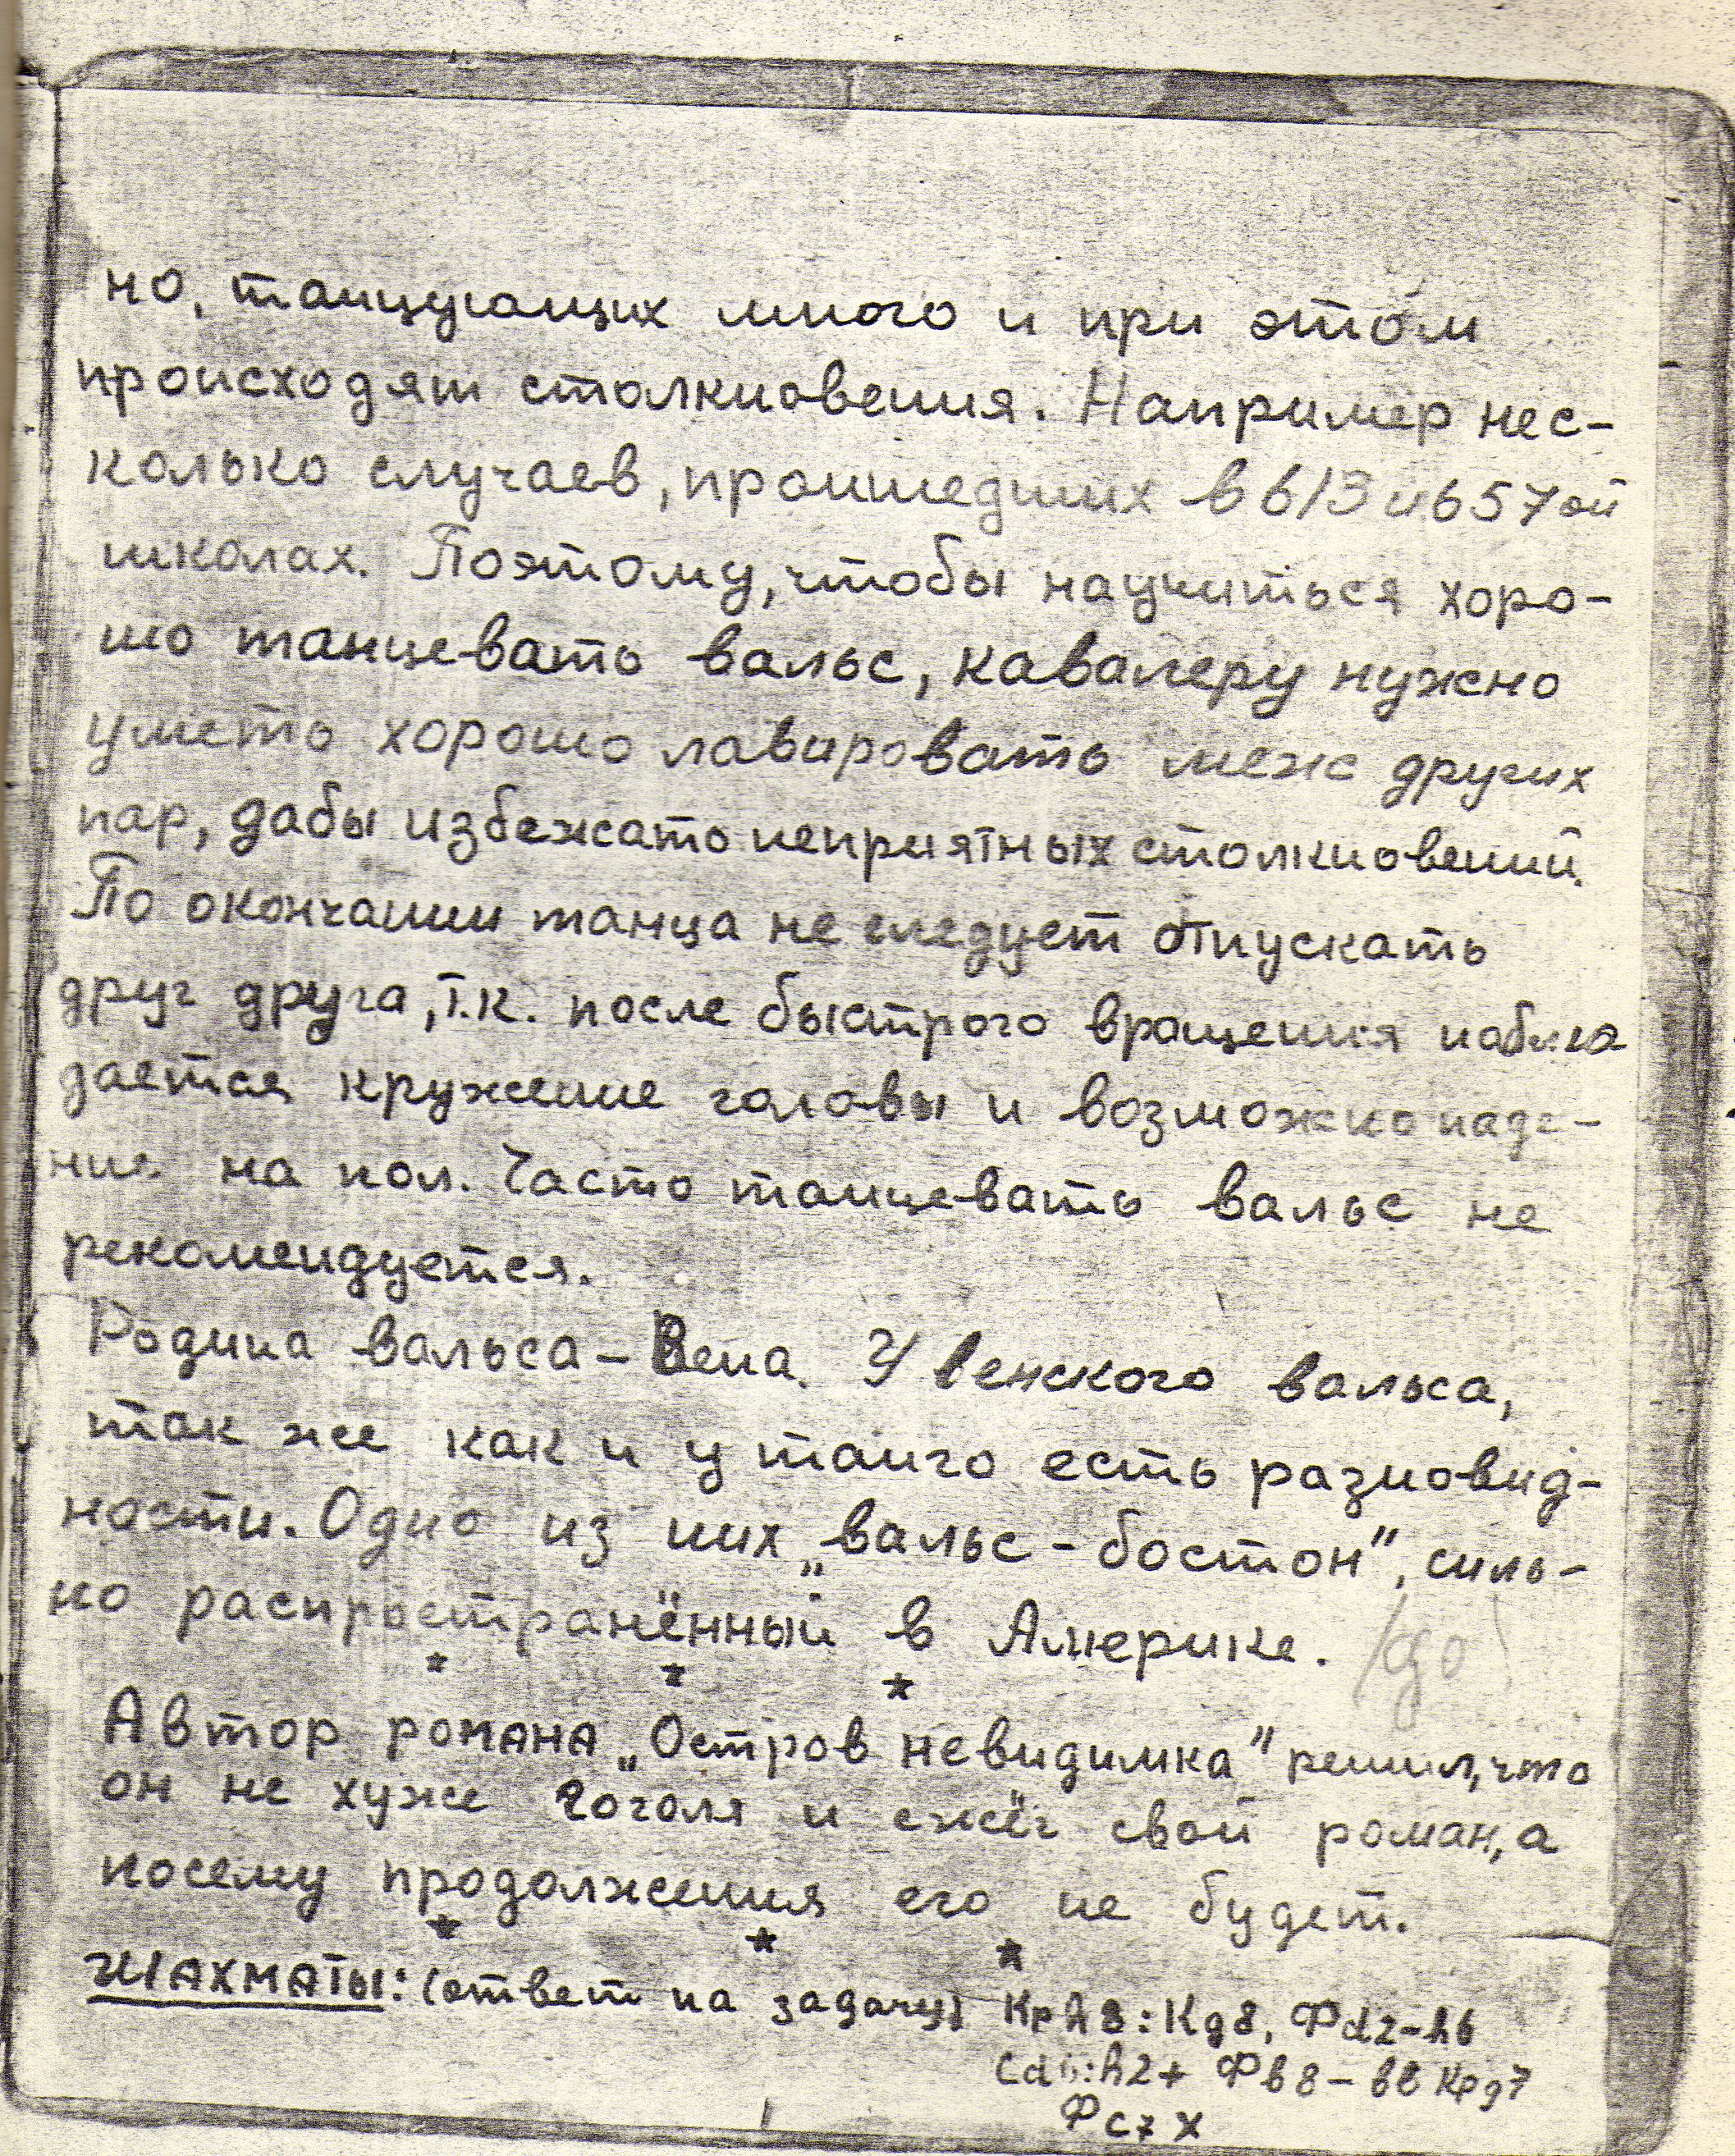
\includegraphics[width=\textwidth]{inc/Vynd/Vynd013}

\section*{Из <<Вундеркинда>> юбилейного. 1987 год.}

\noindent
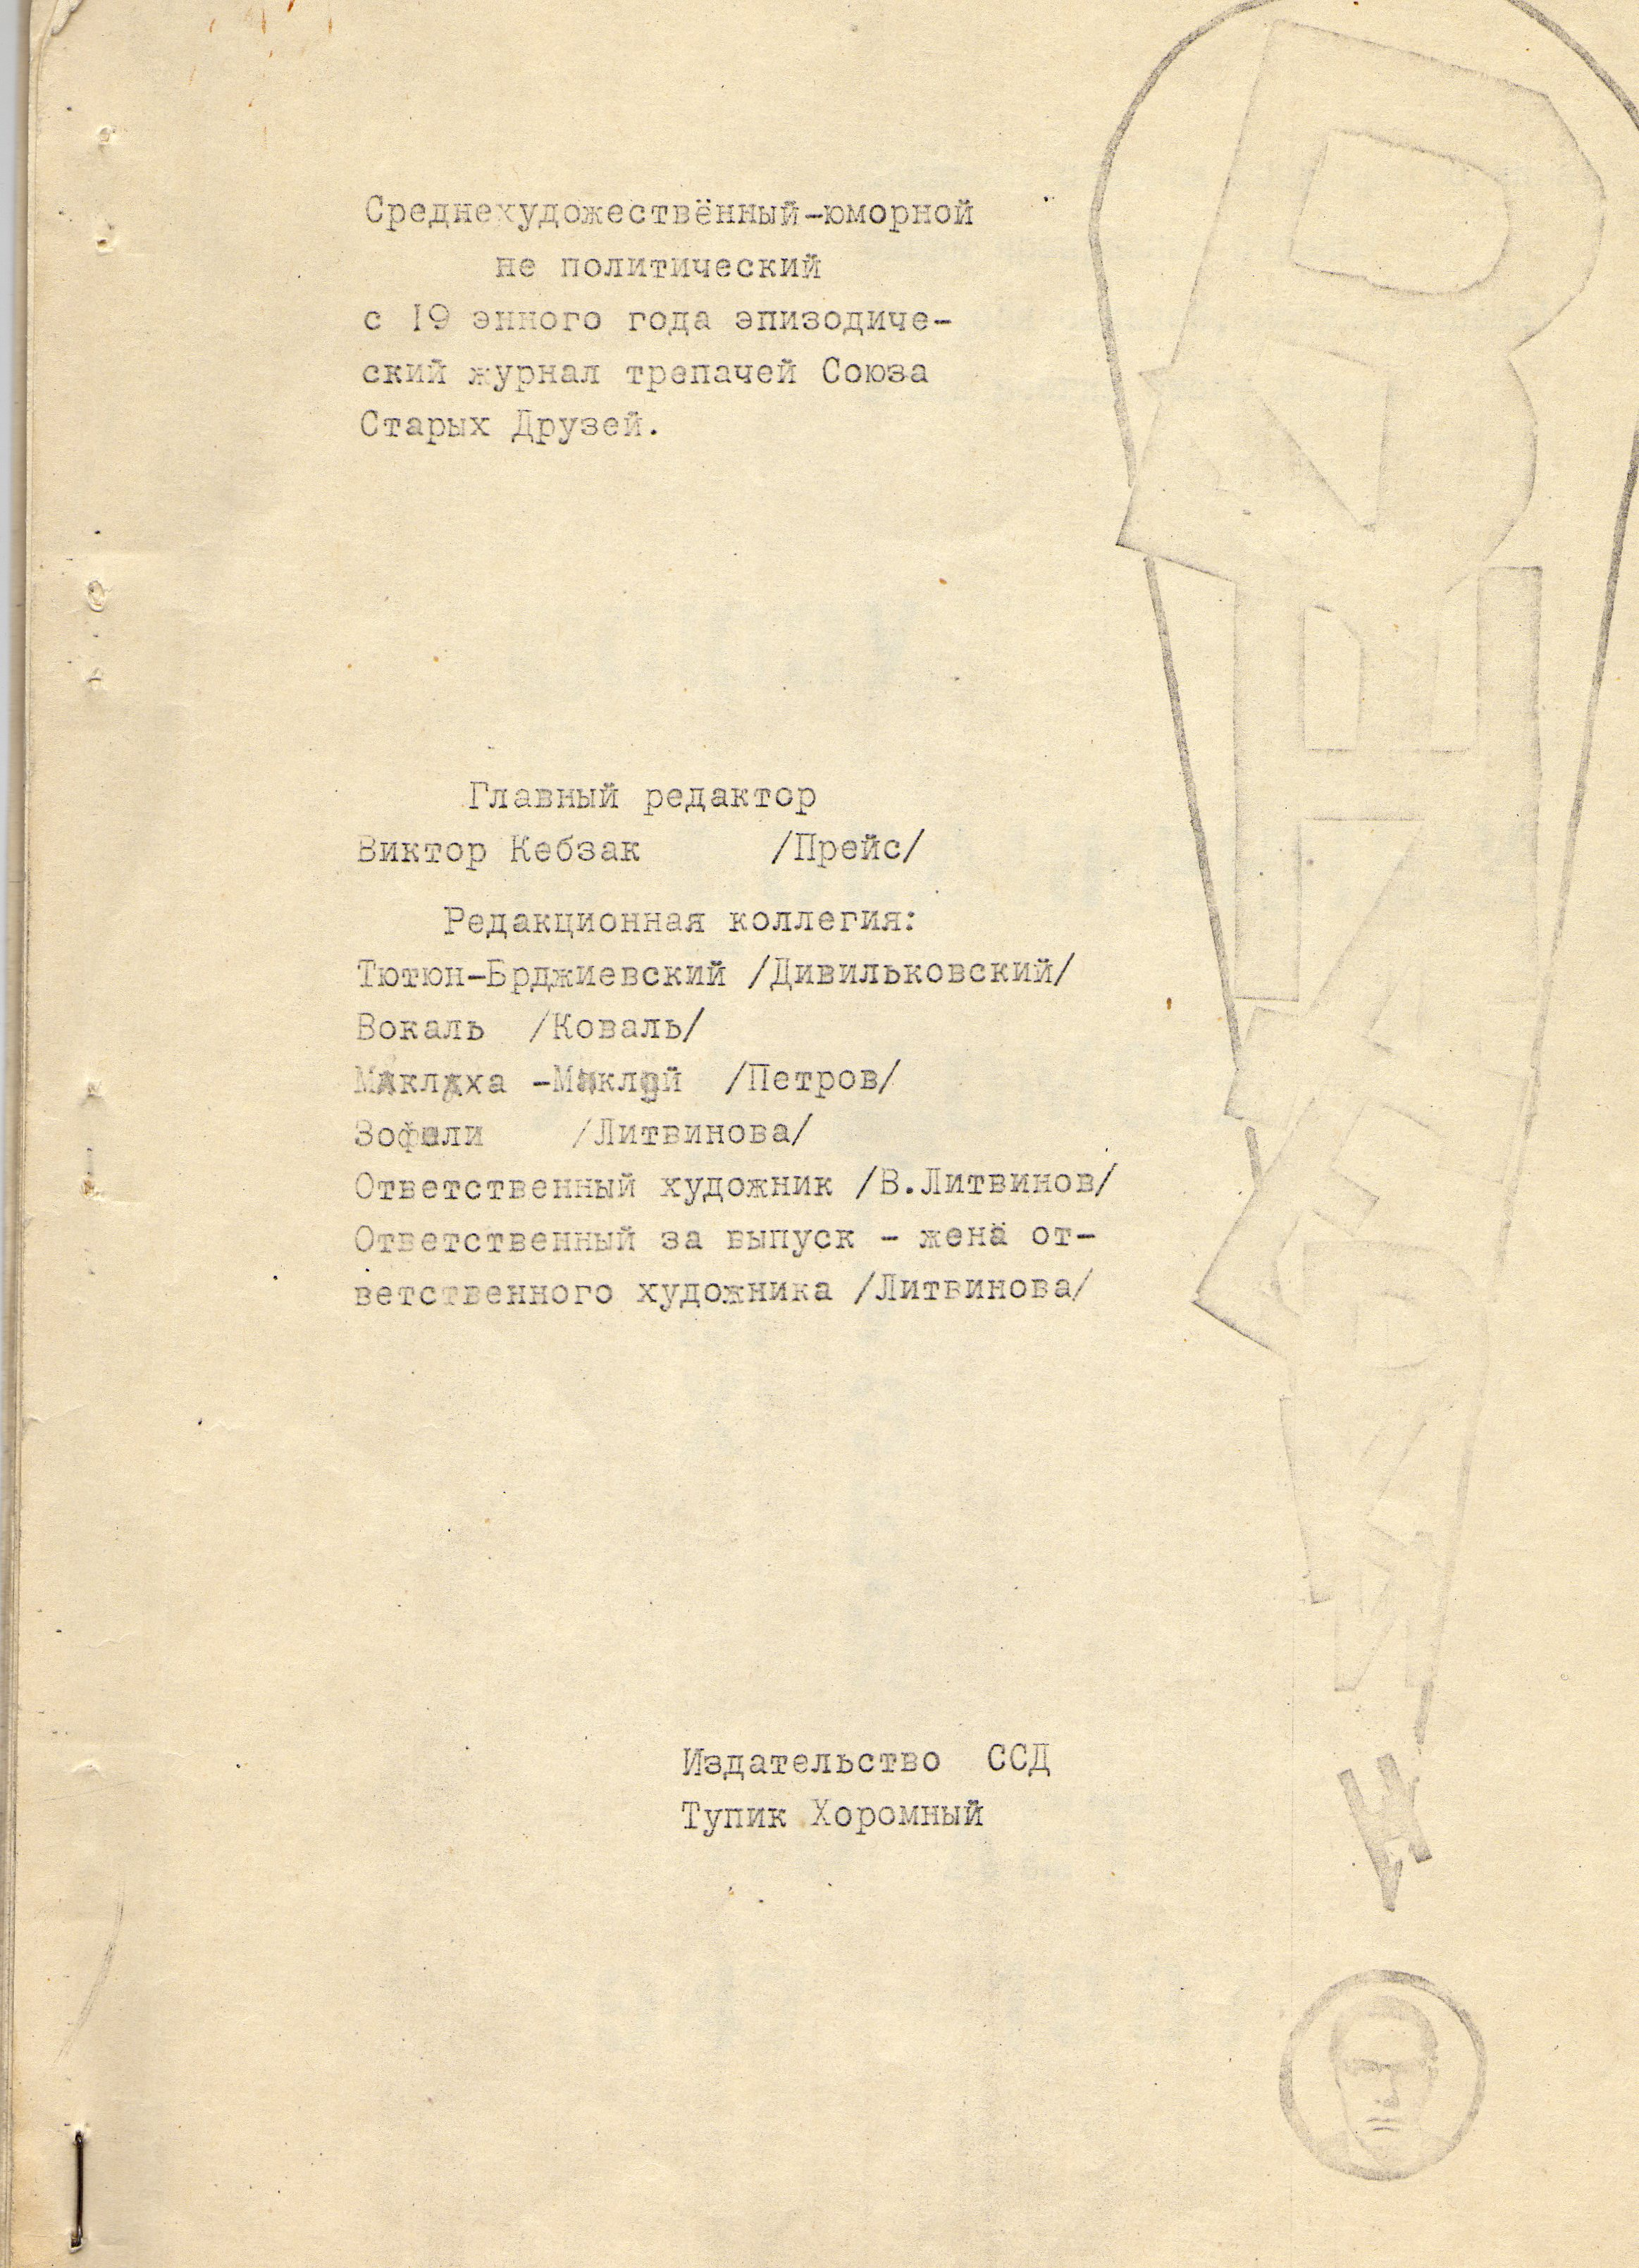
\includegraphics[width=\textwidth]{inc/Vynd/Vynd014}

\noindent
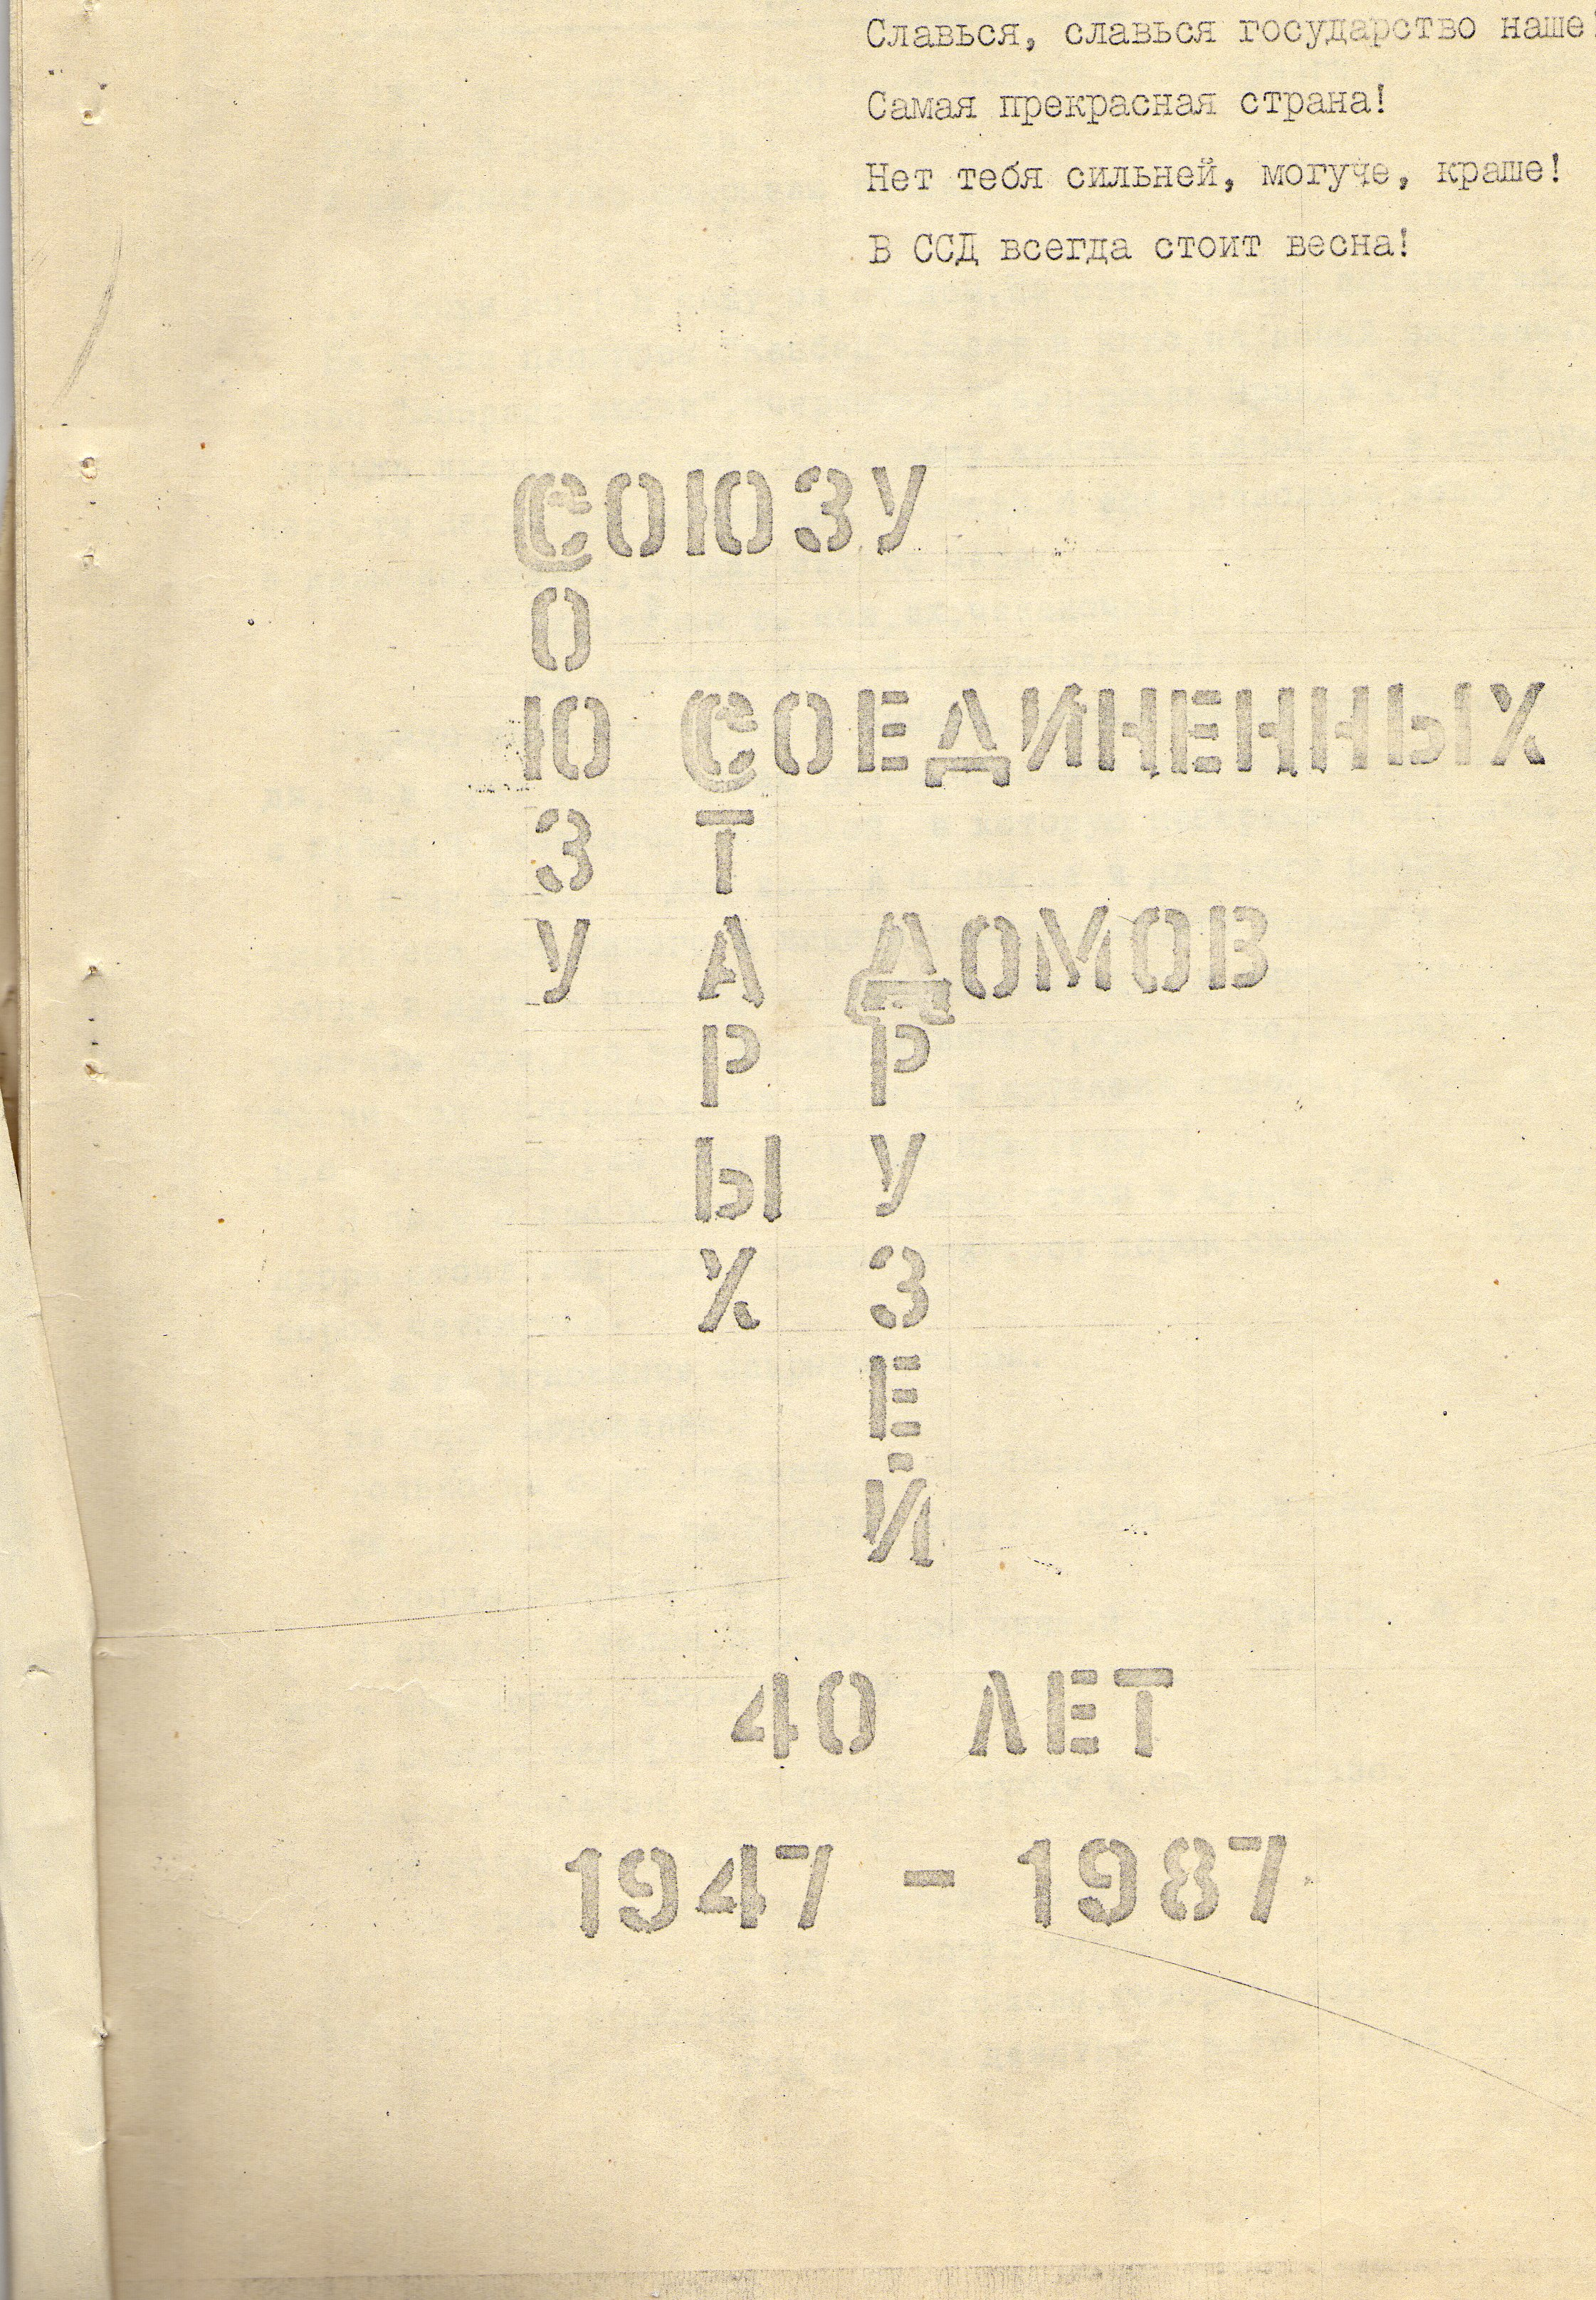
\includegraphics[width=\textwidth]{inc/Vynd/Vynd016}

\noindent
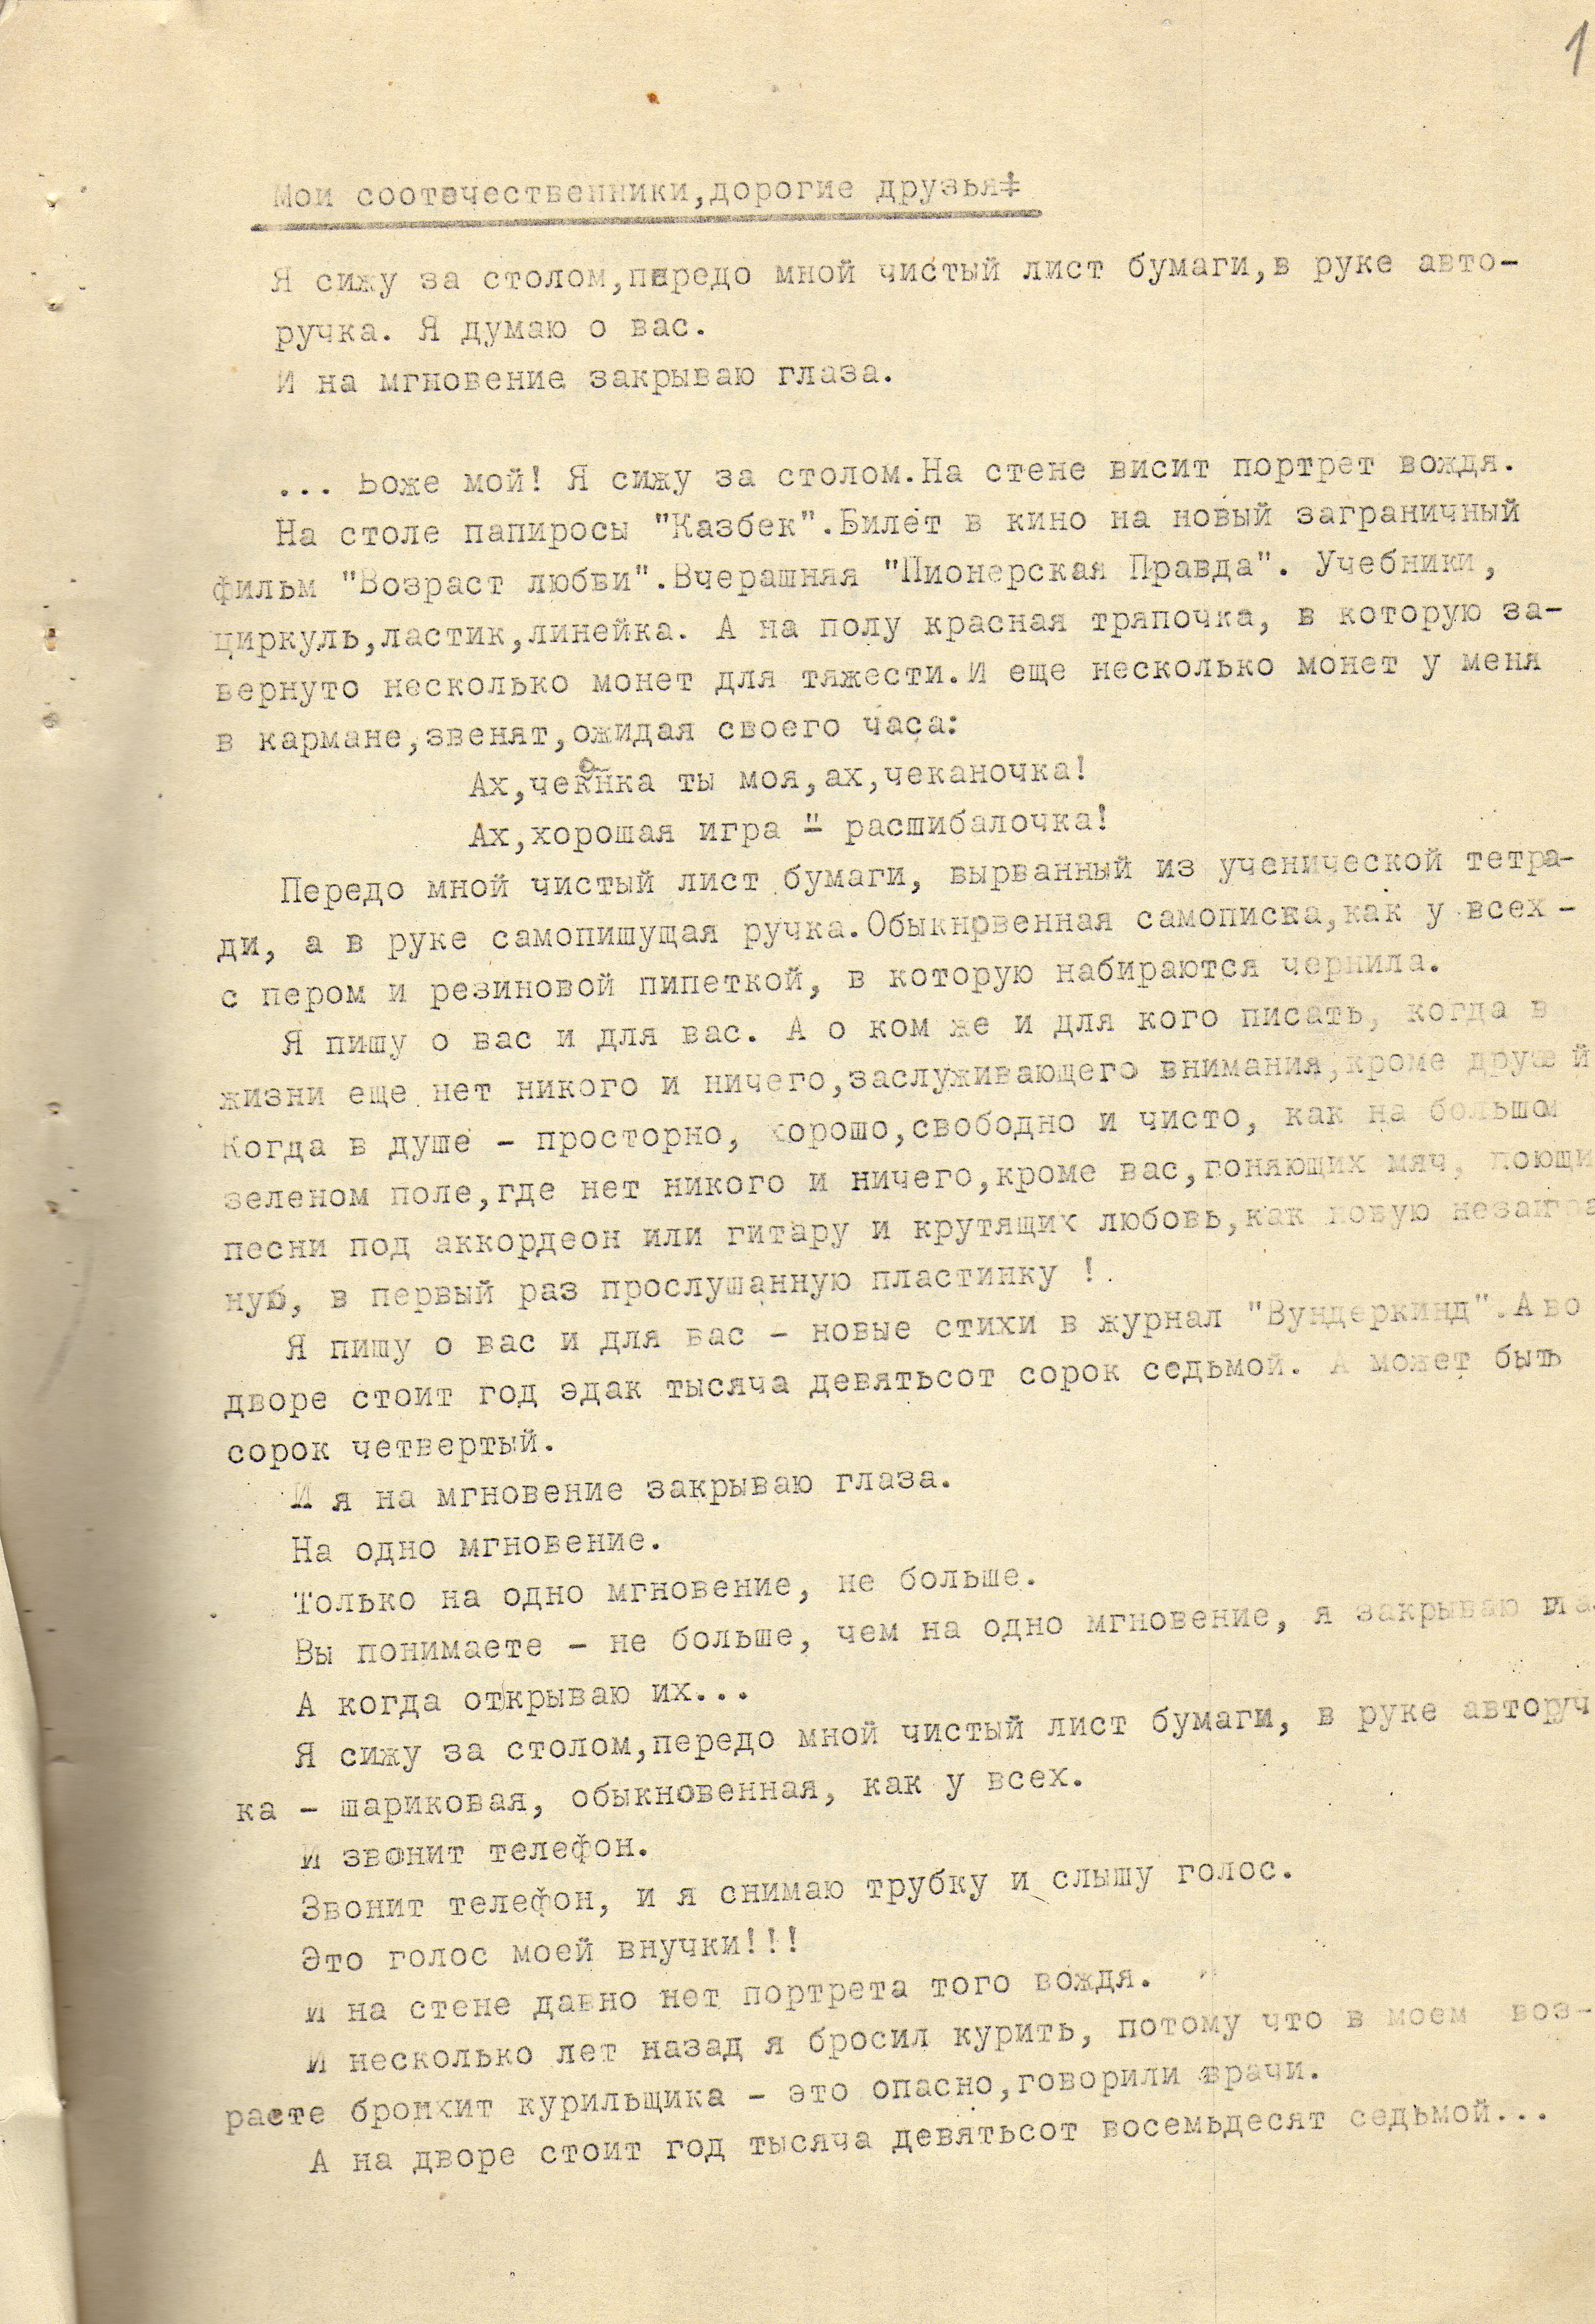
\includegraphics[width=\textwidth]{inc/Vynd/Vynd017}

\noindent
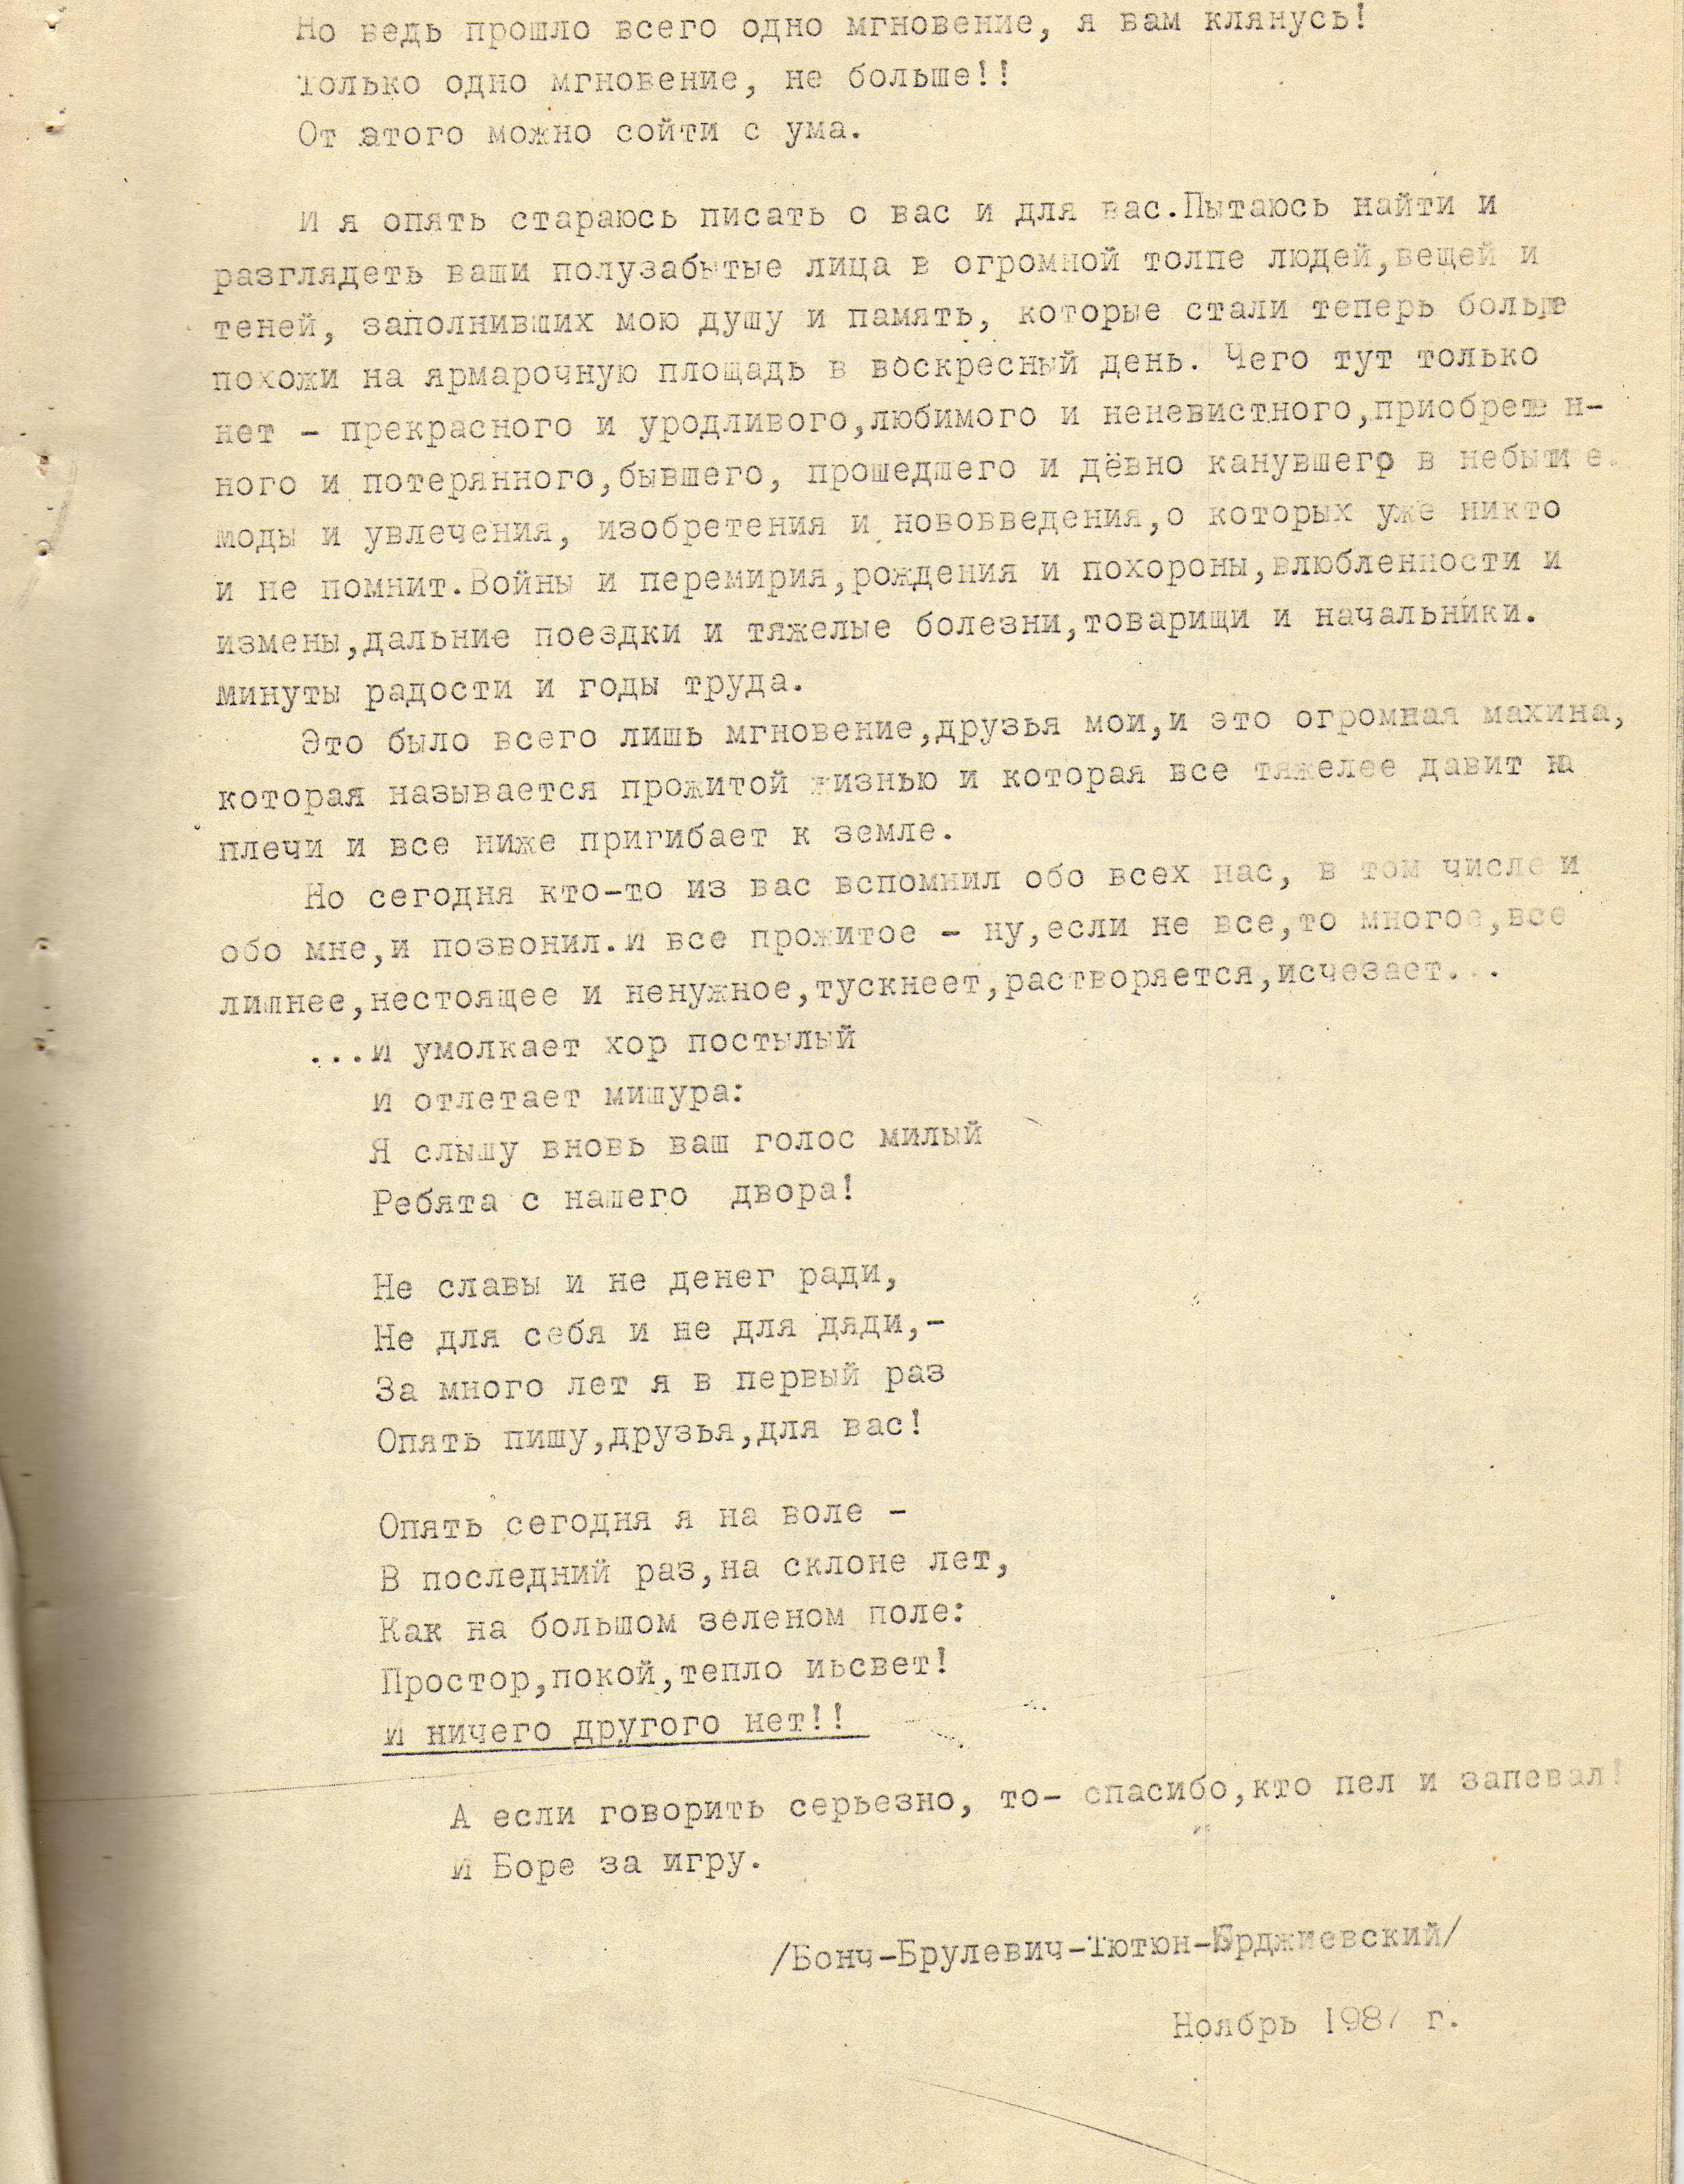
\includegraphics[width=\textwidth]{inc/Vynd/Vynd018}

\noindent
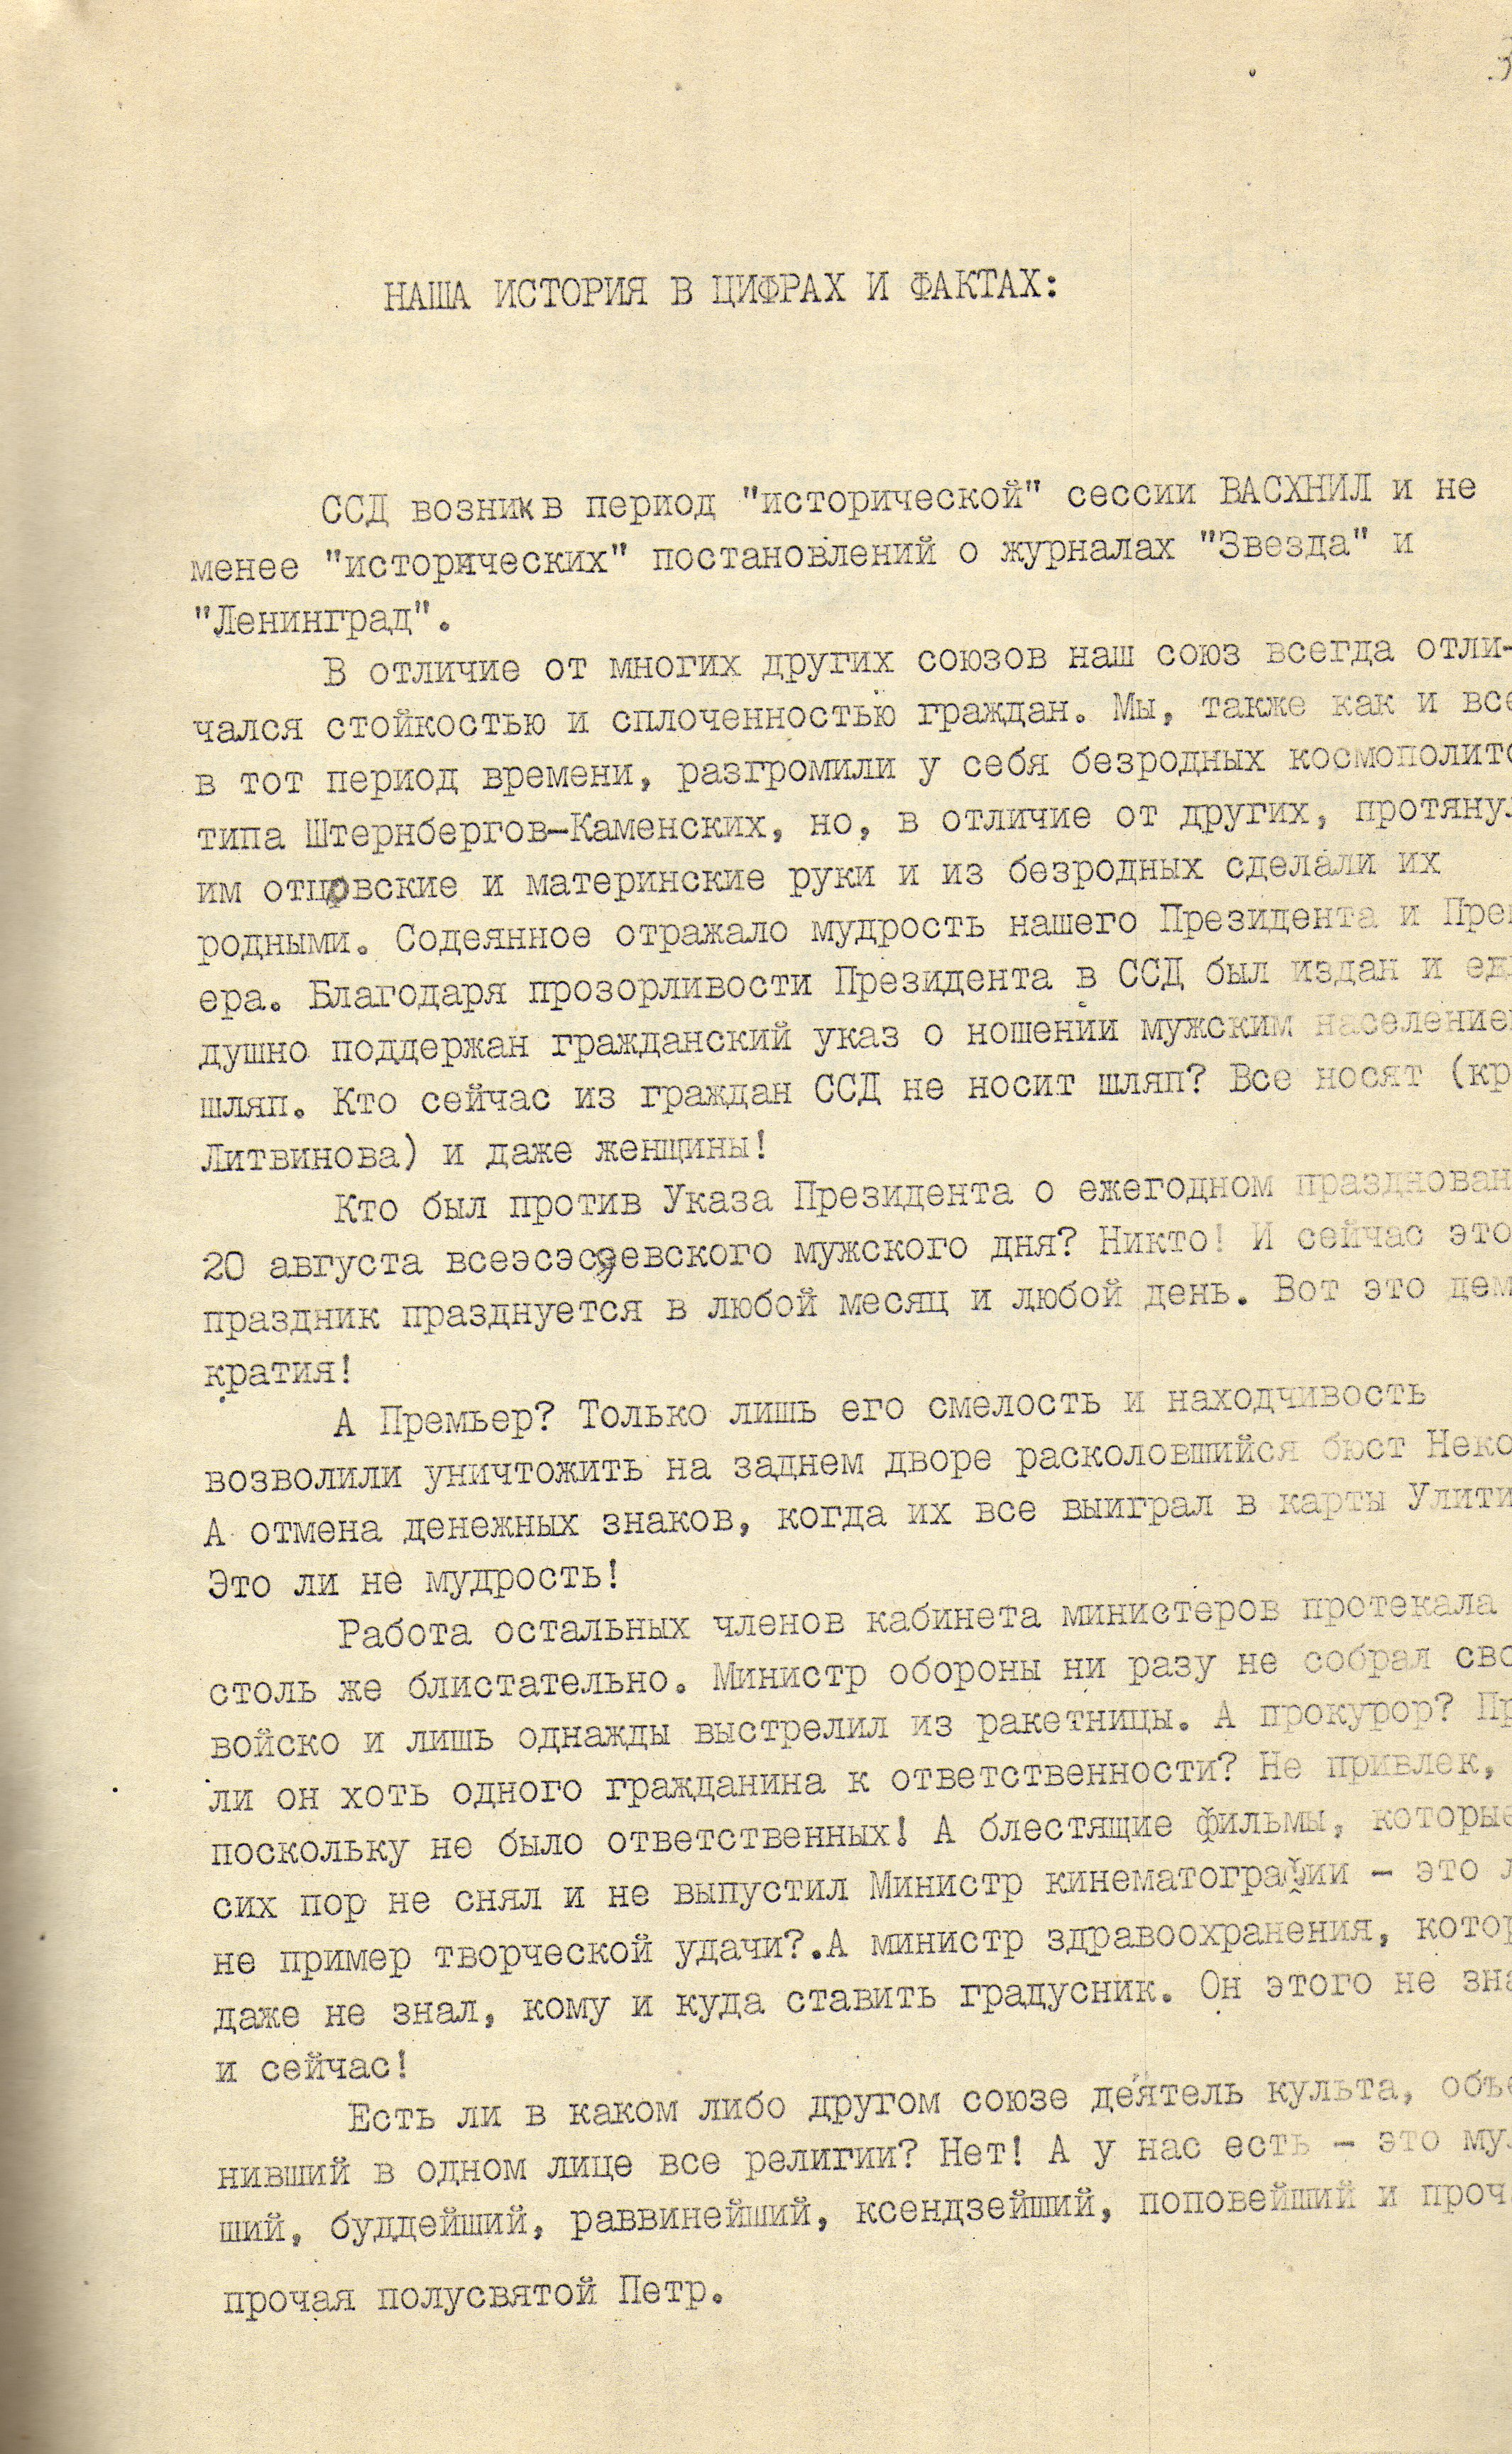
\includegraphics[width=\textwidth]{inc/Vynd/Vynd019}

\noindent
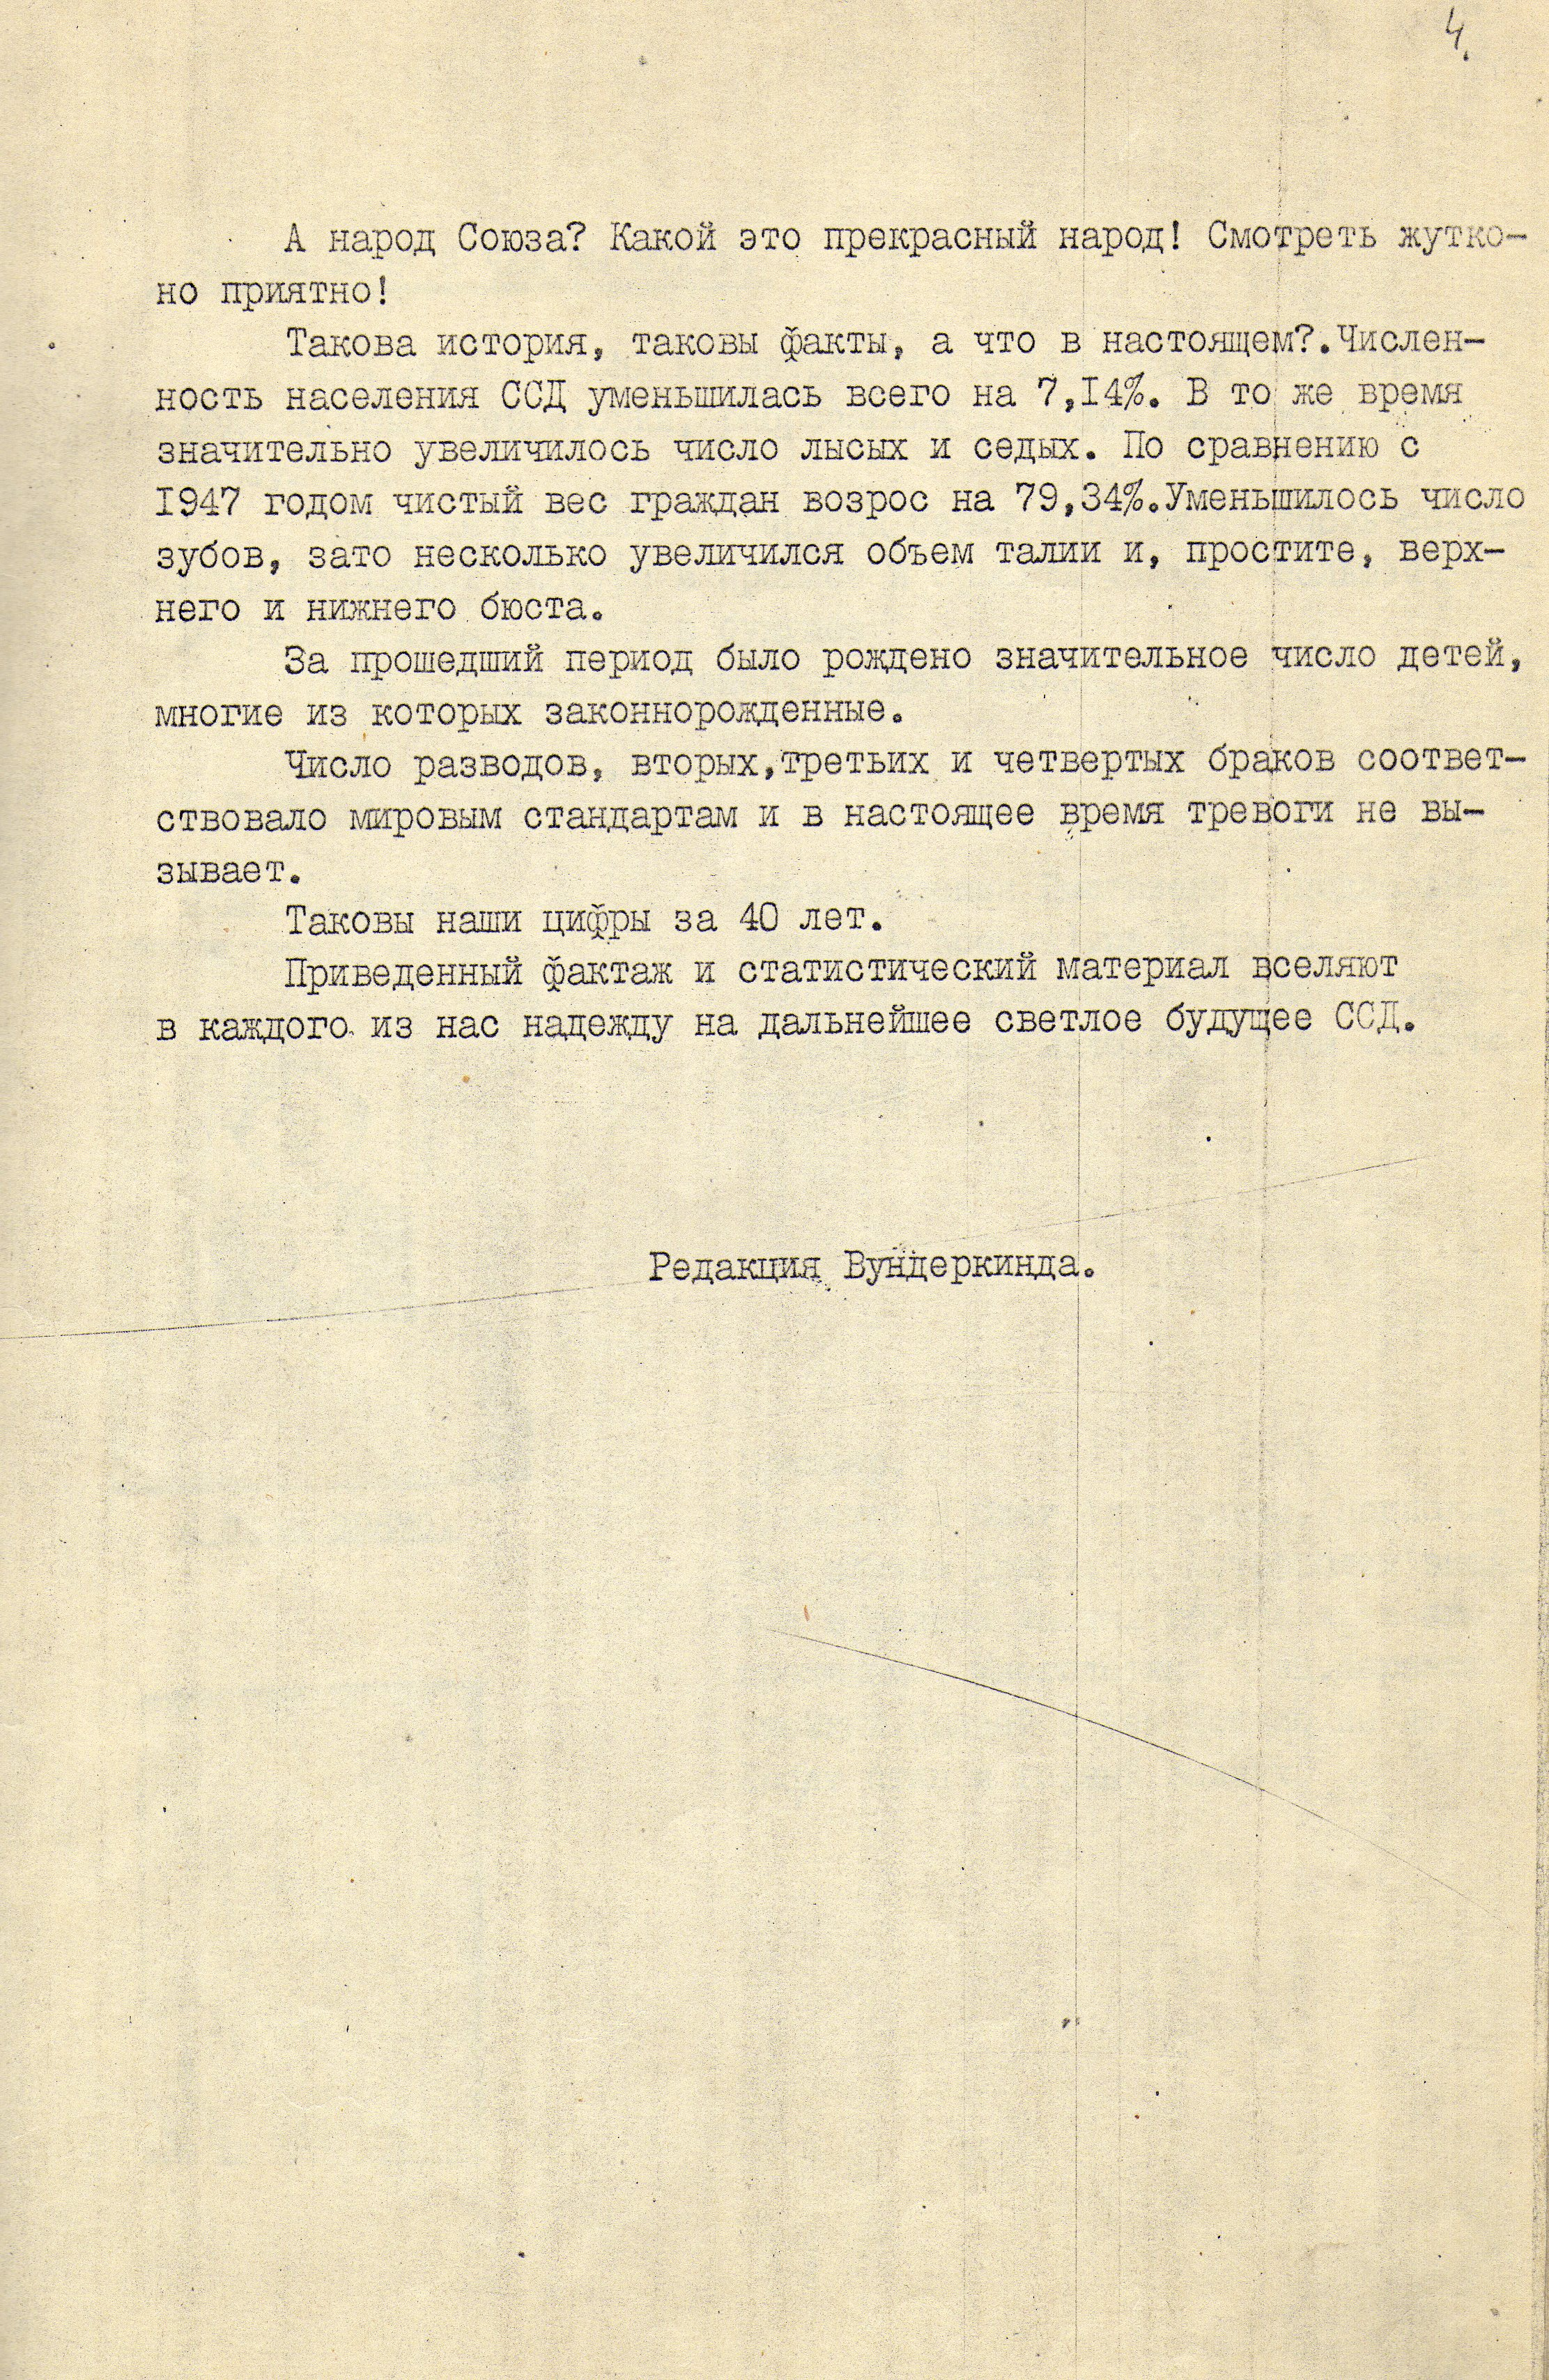
\includegraphics[width=\textwidth]{inc/Vynd/Vynd020}

\noindent
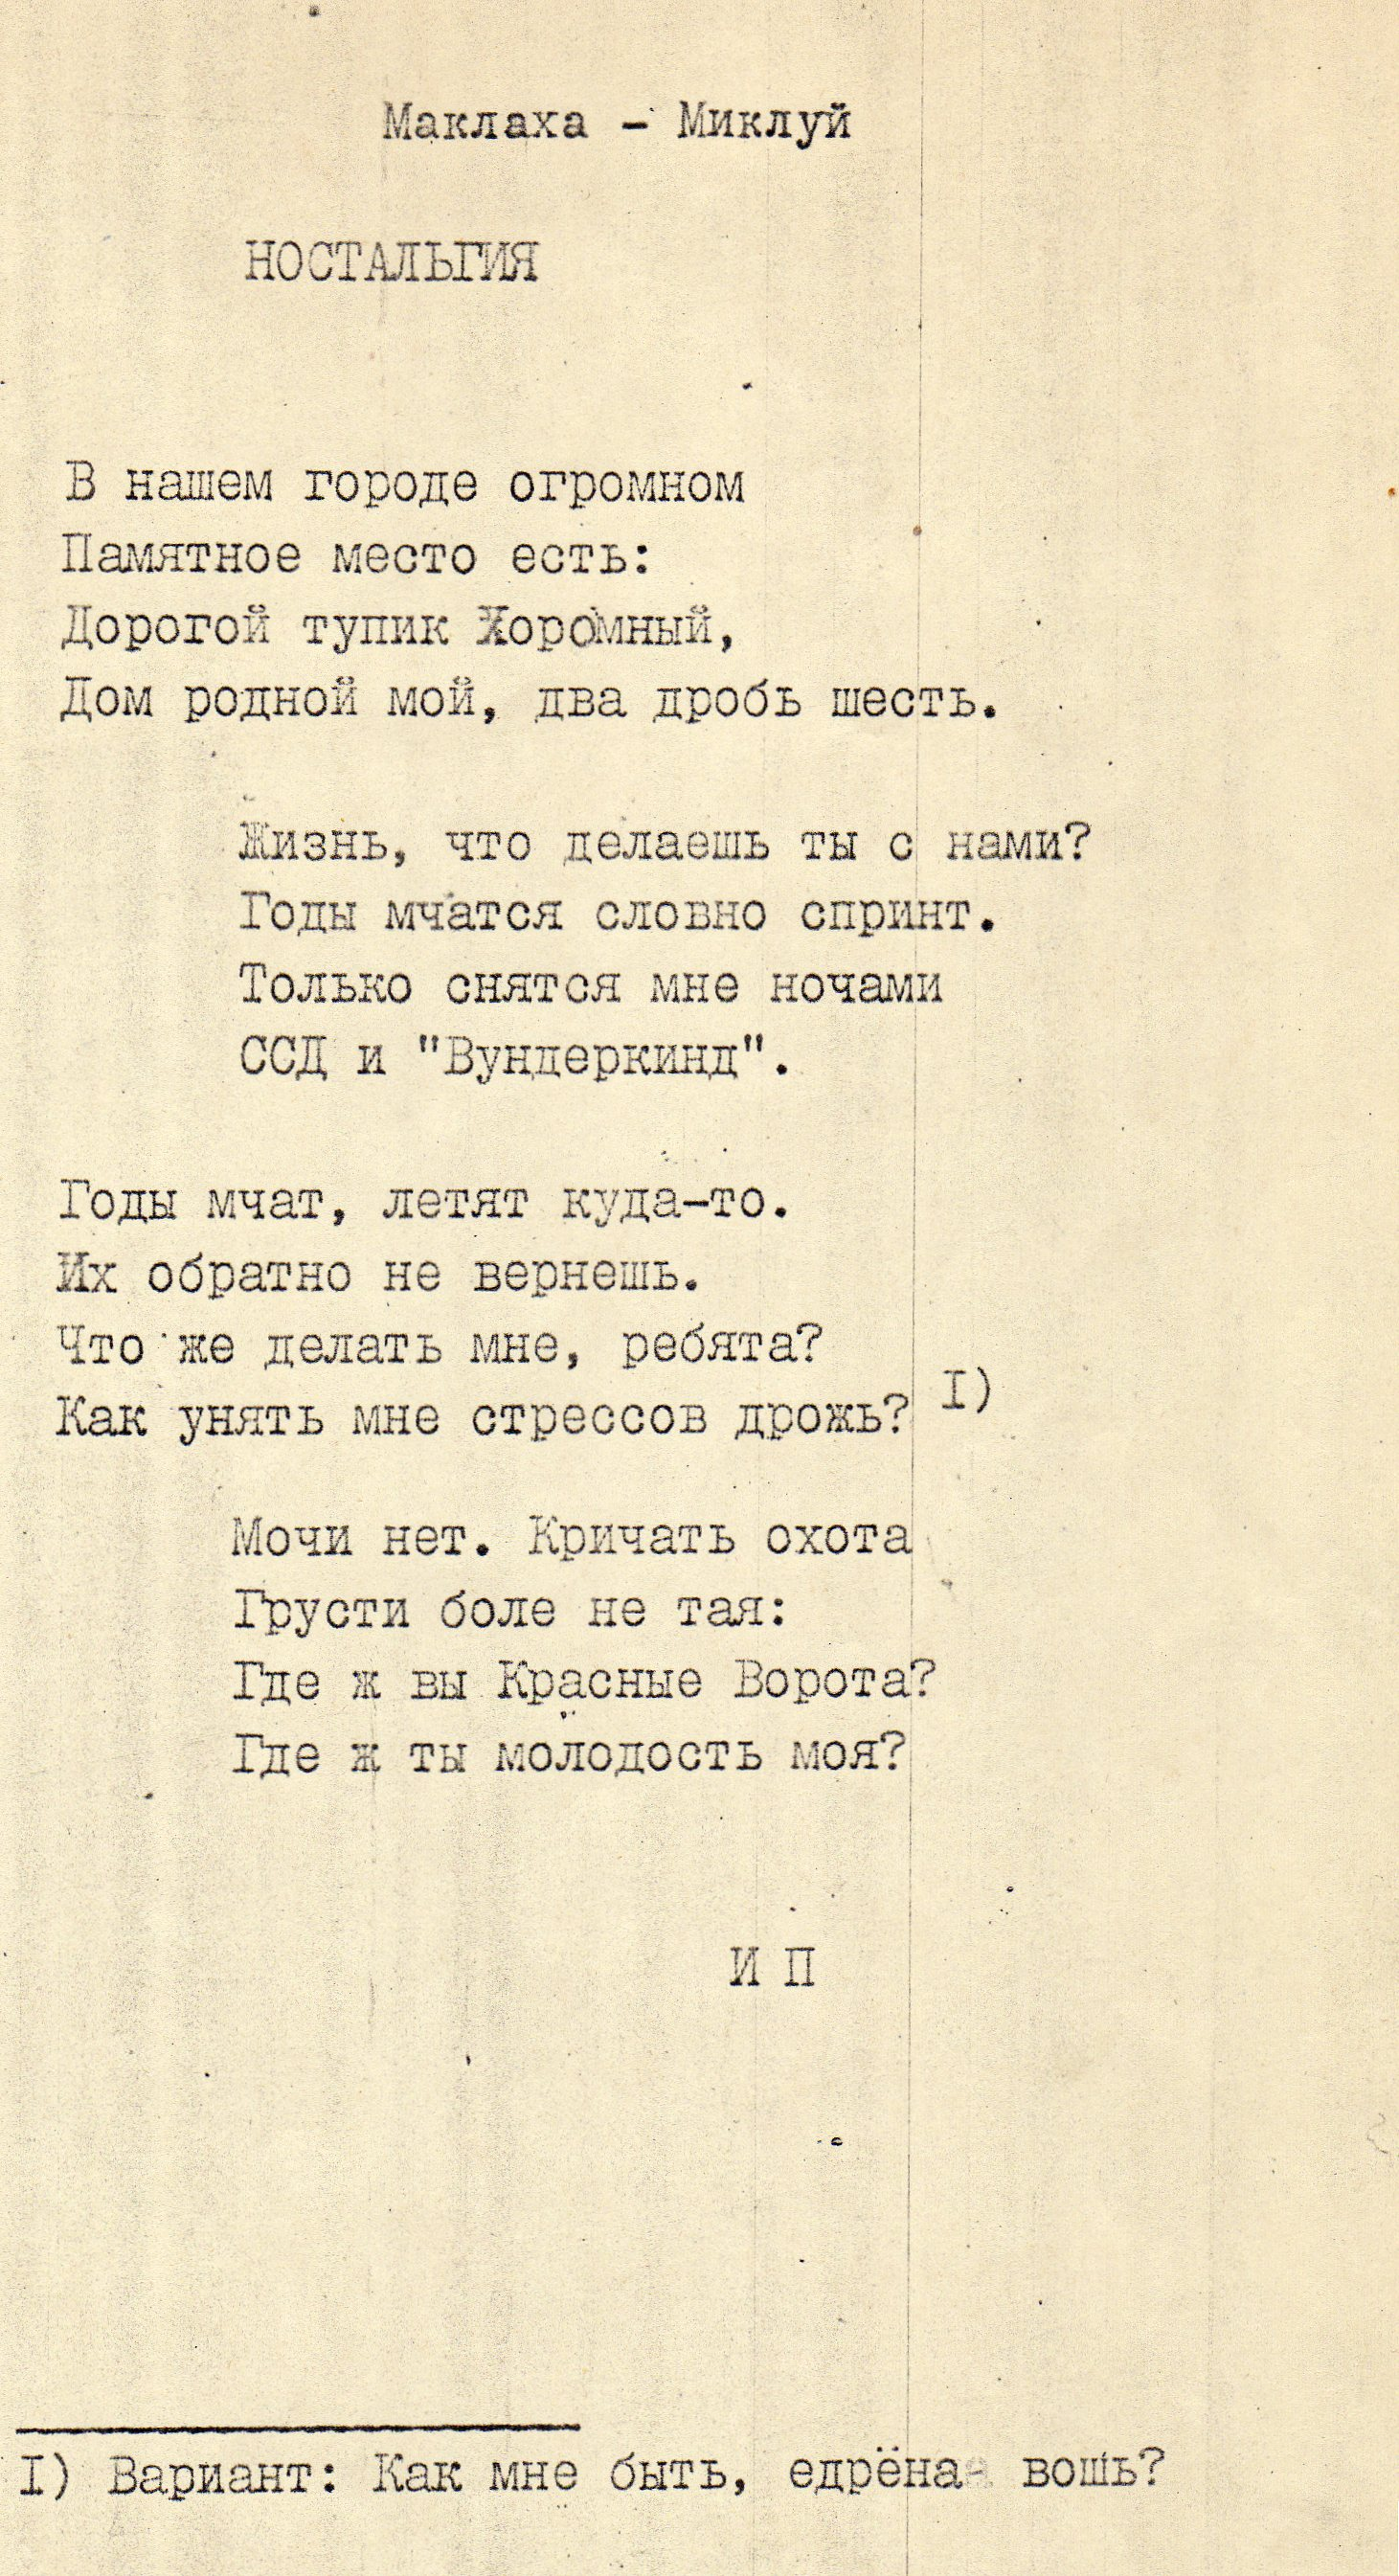
\includegraphics[width=\textwidth]{inc/Vynd/Vynd021}

\noindent
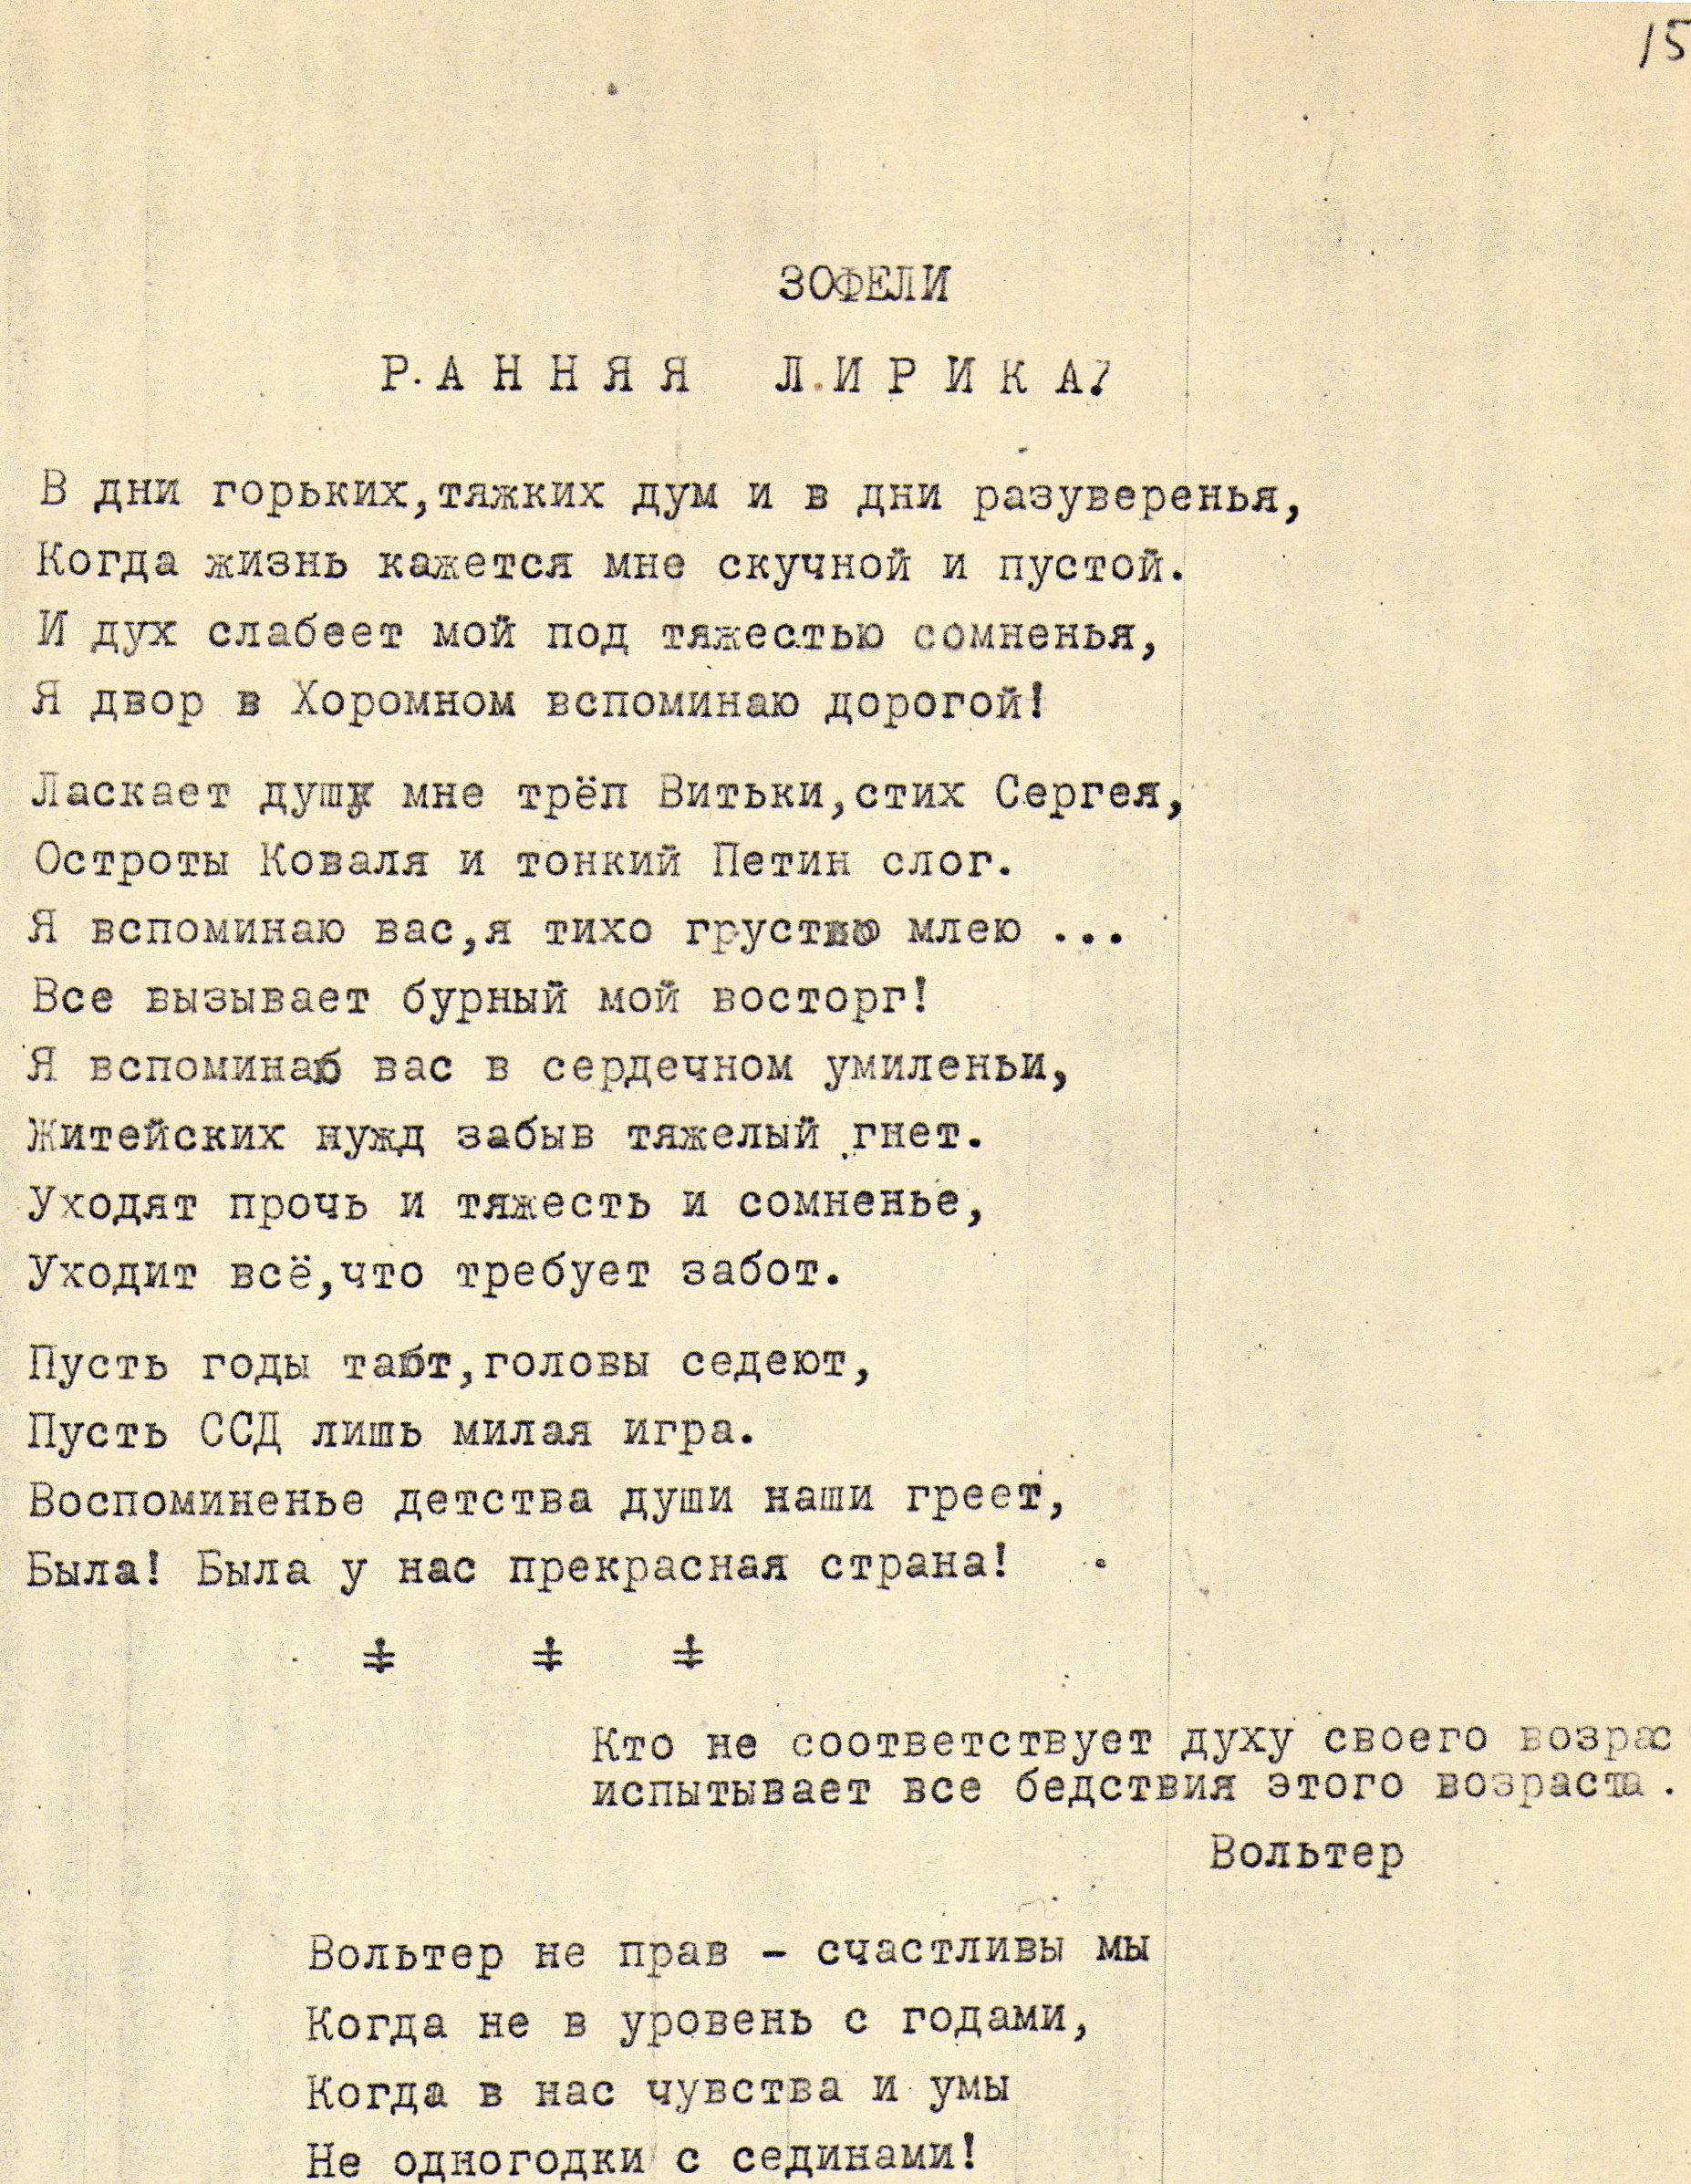
\includegraphics[width=\textwidth]{inc/Vynd/Vynd022}

\noindent
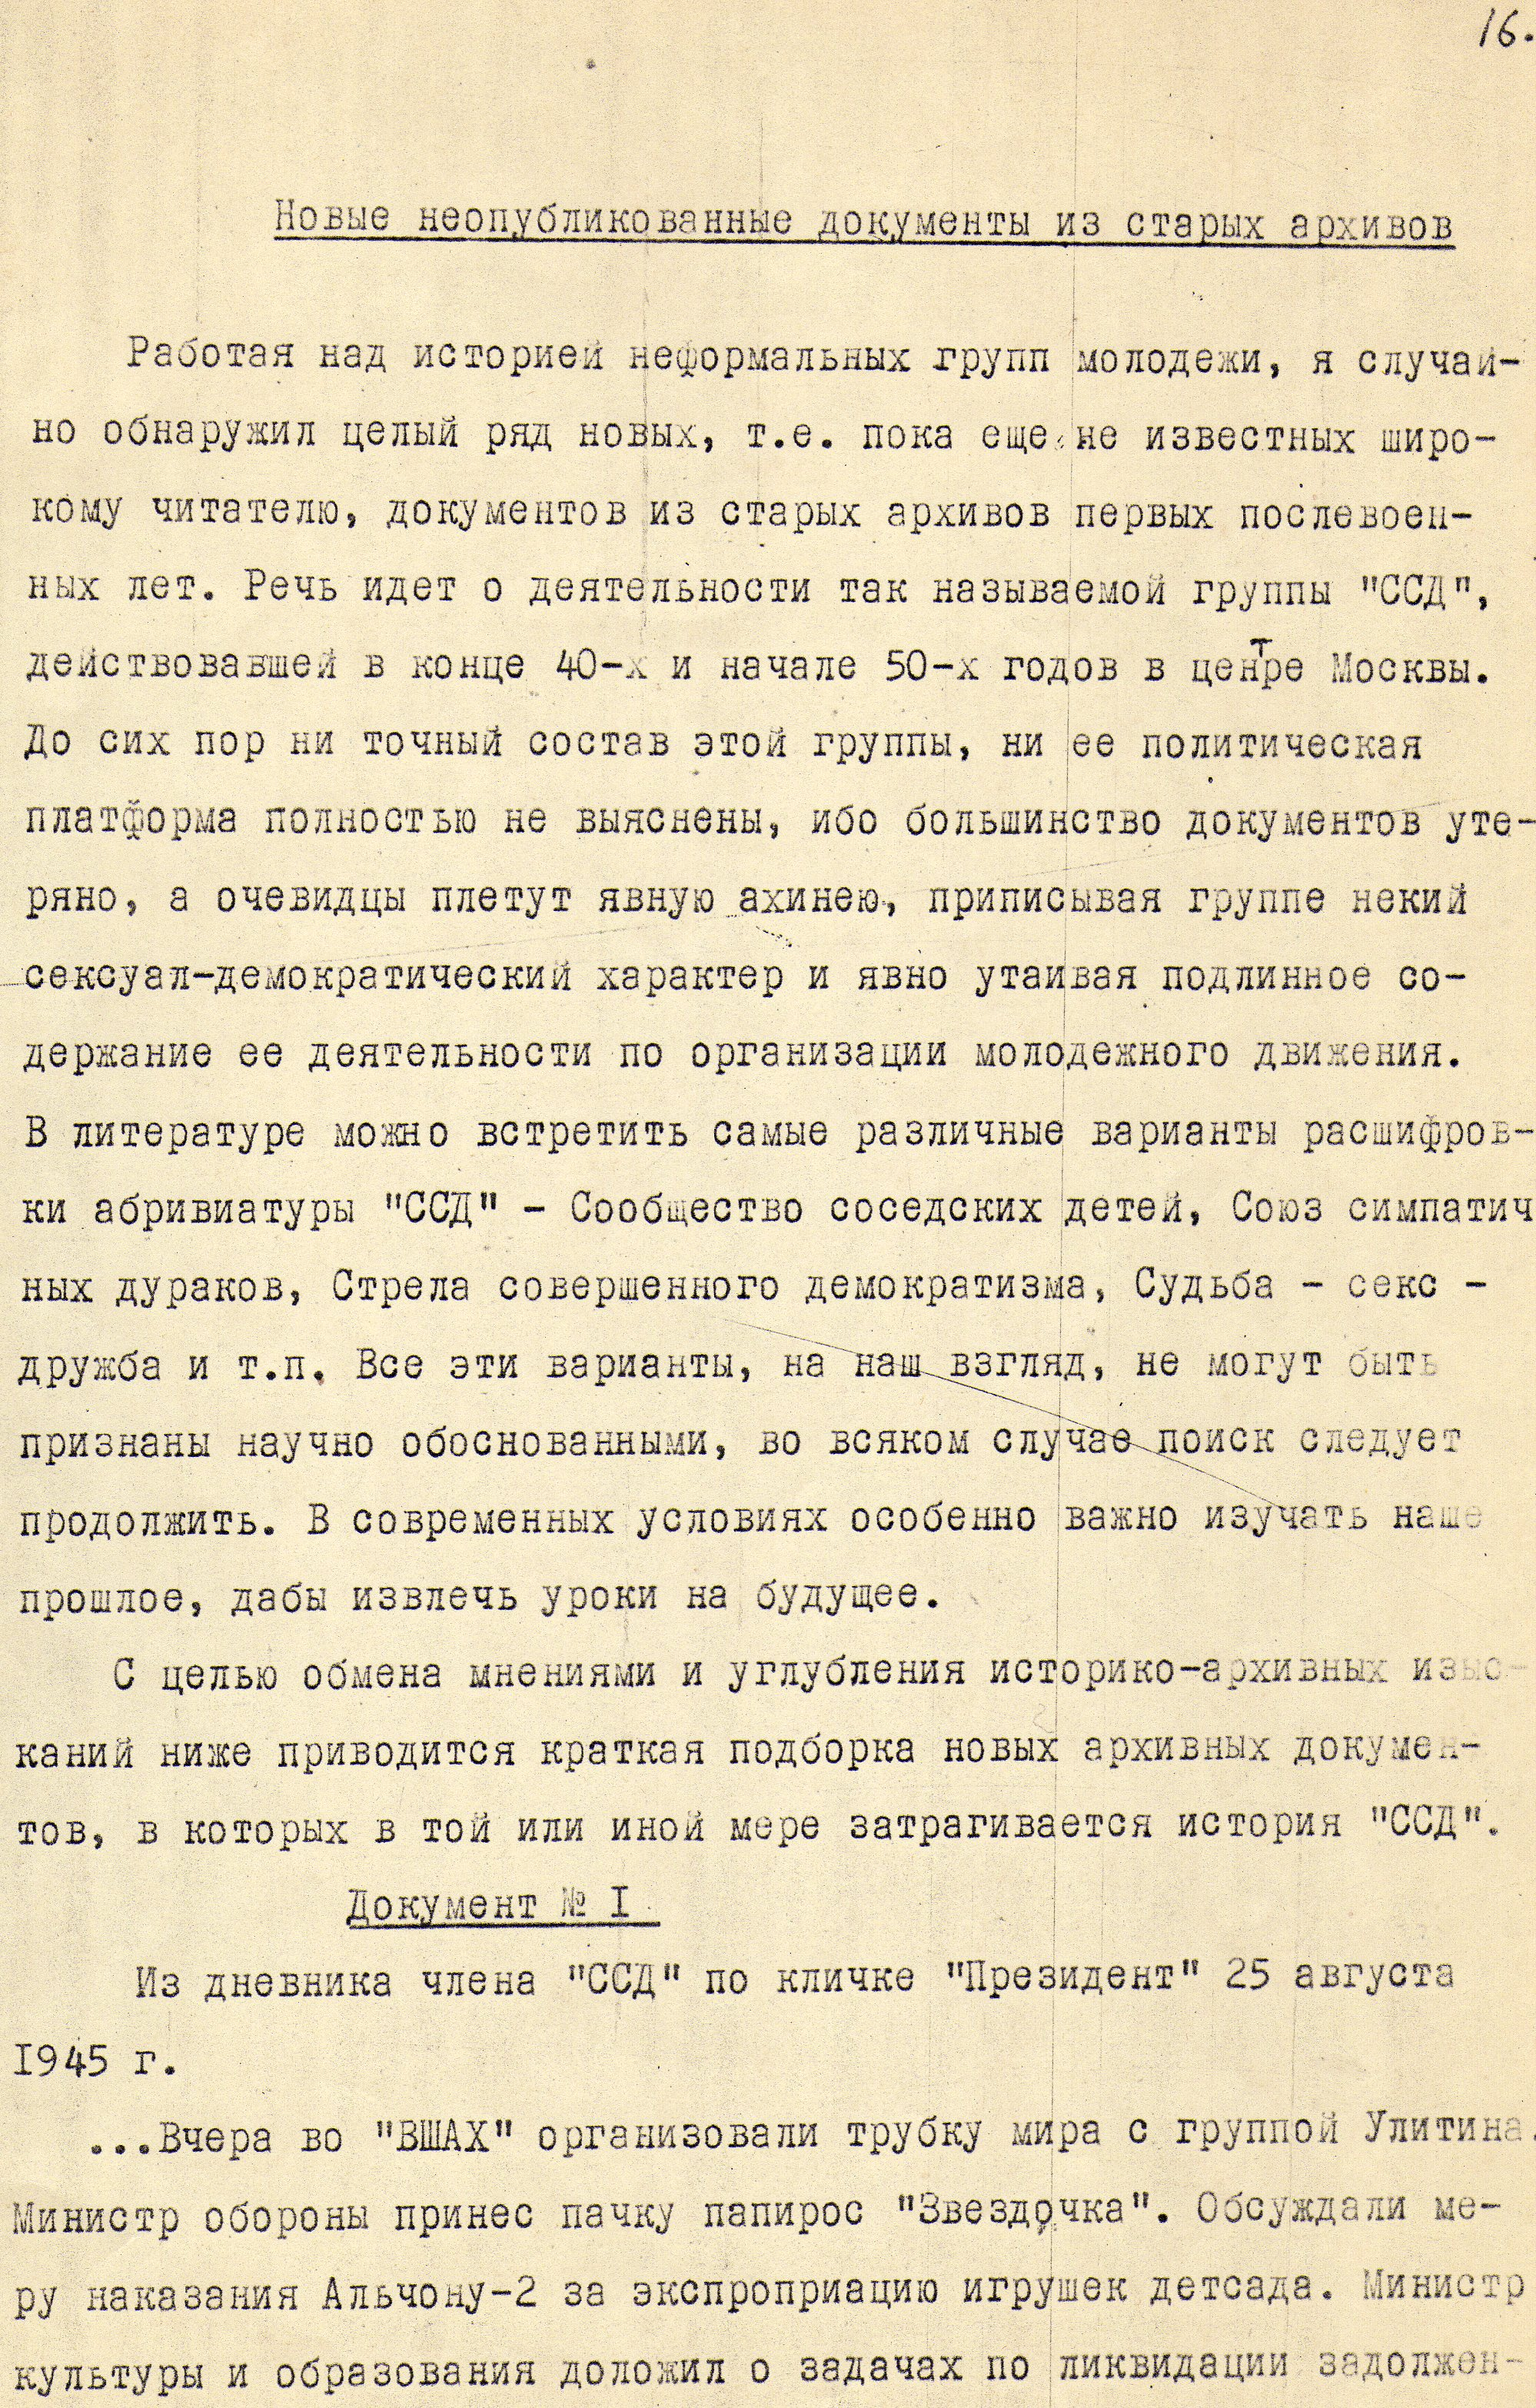
\includegraphics[width=\textwidth]{inc/Vynd/Vynd023}

\noindent
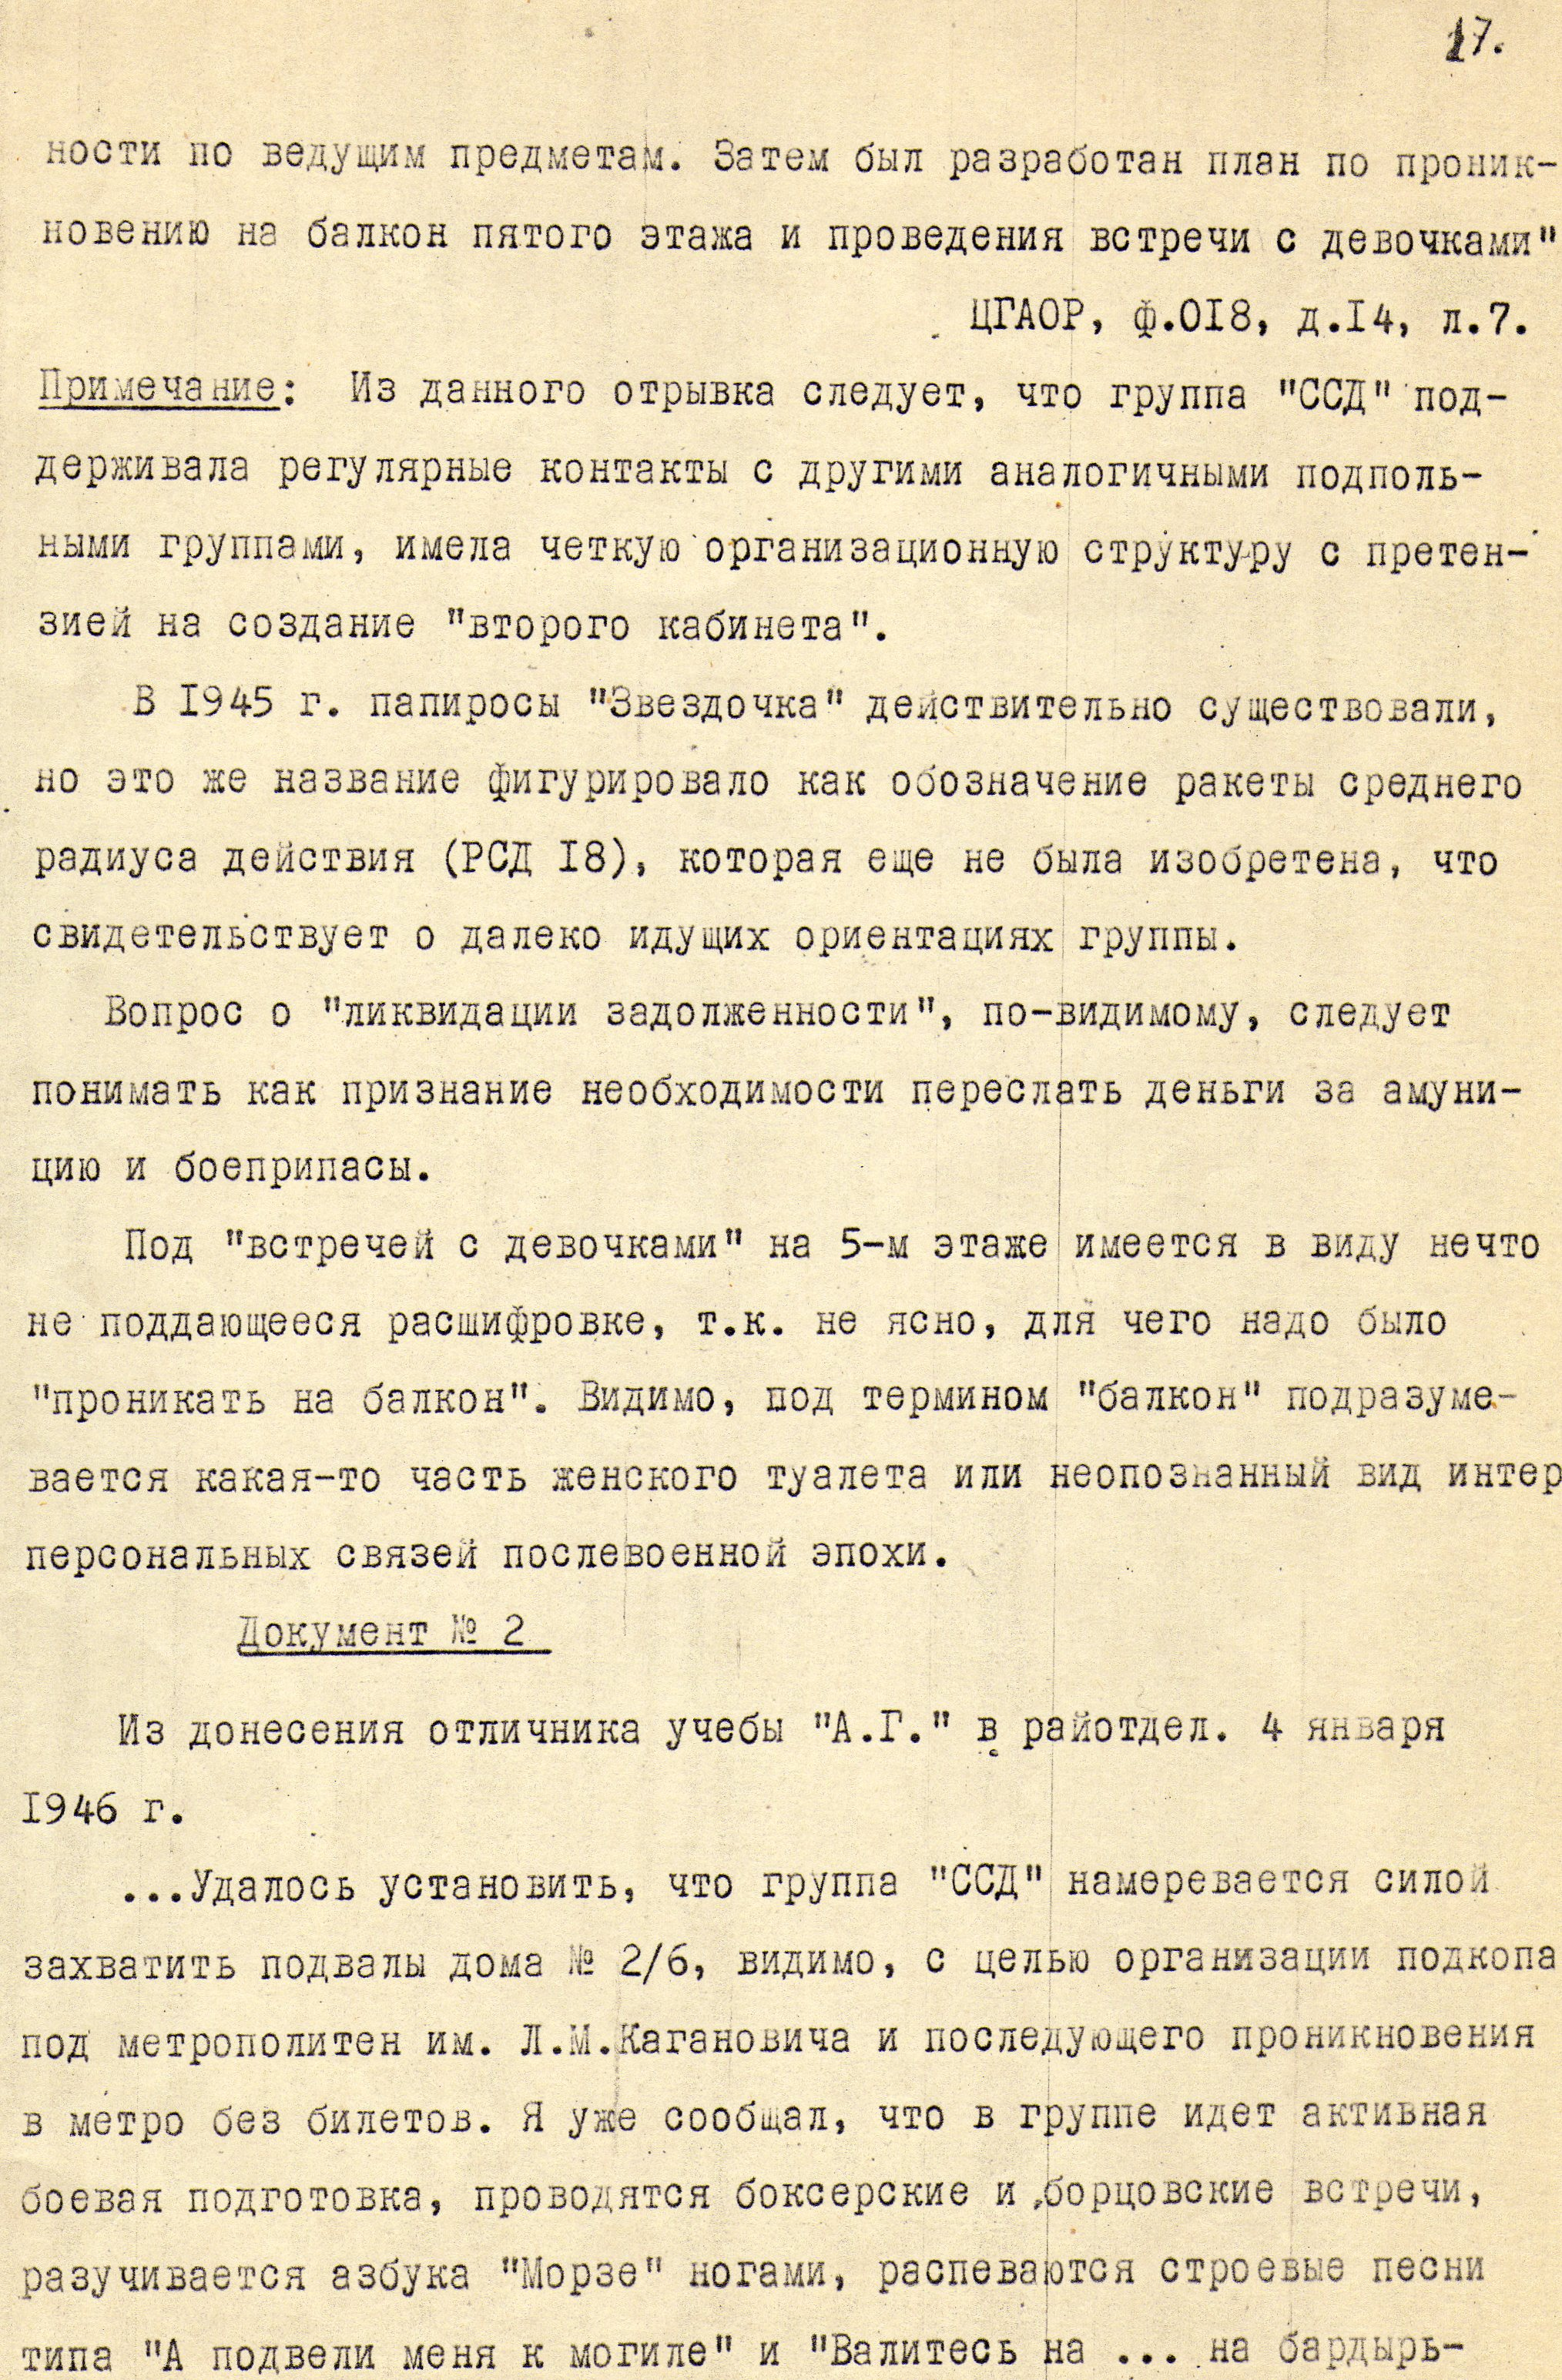
\includegraphics[width=\textwidth]{inc/Vynd/Vynd024}

\noindent
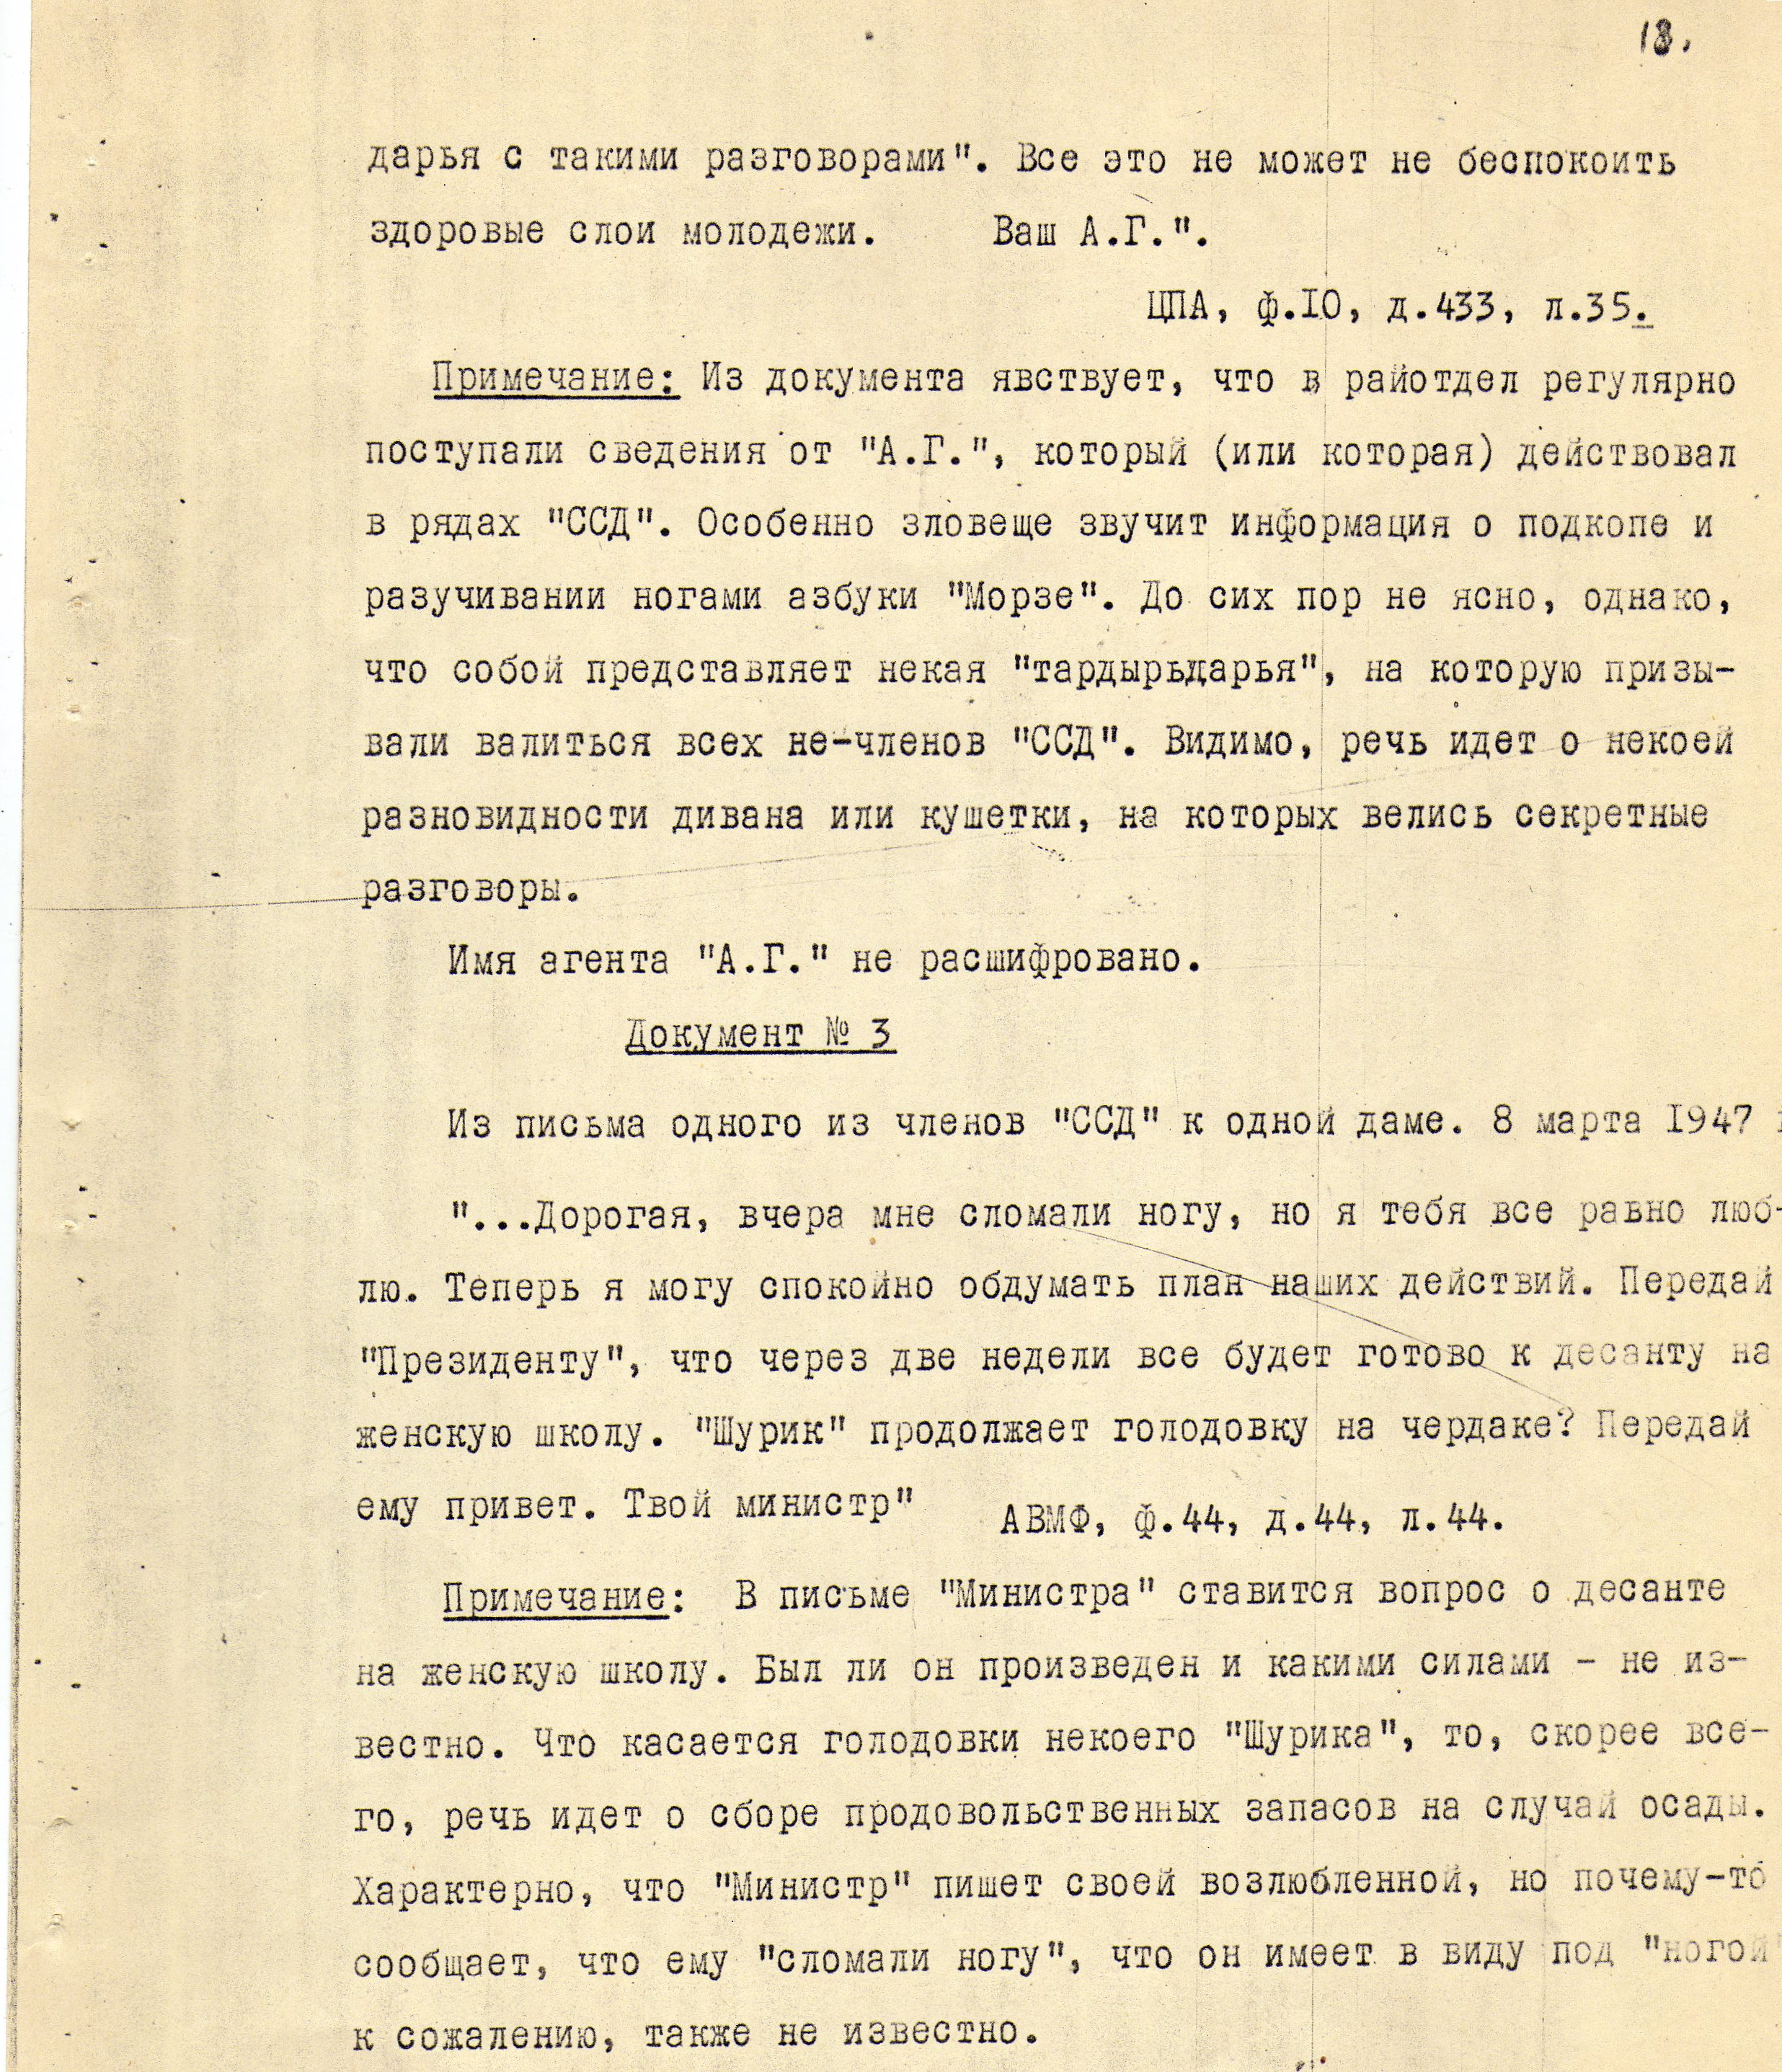
\includegraphics[width=\textwidth]{inc/Vynd/Vynd025}

\noindent
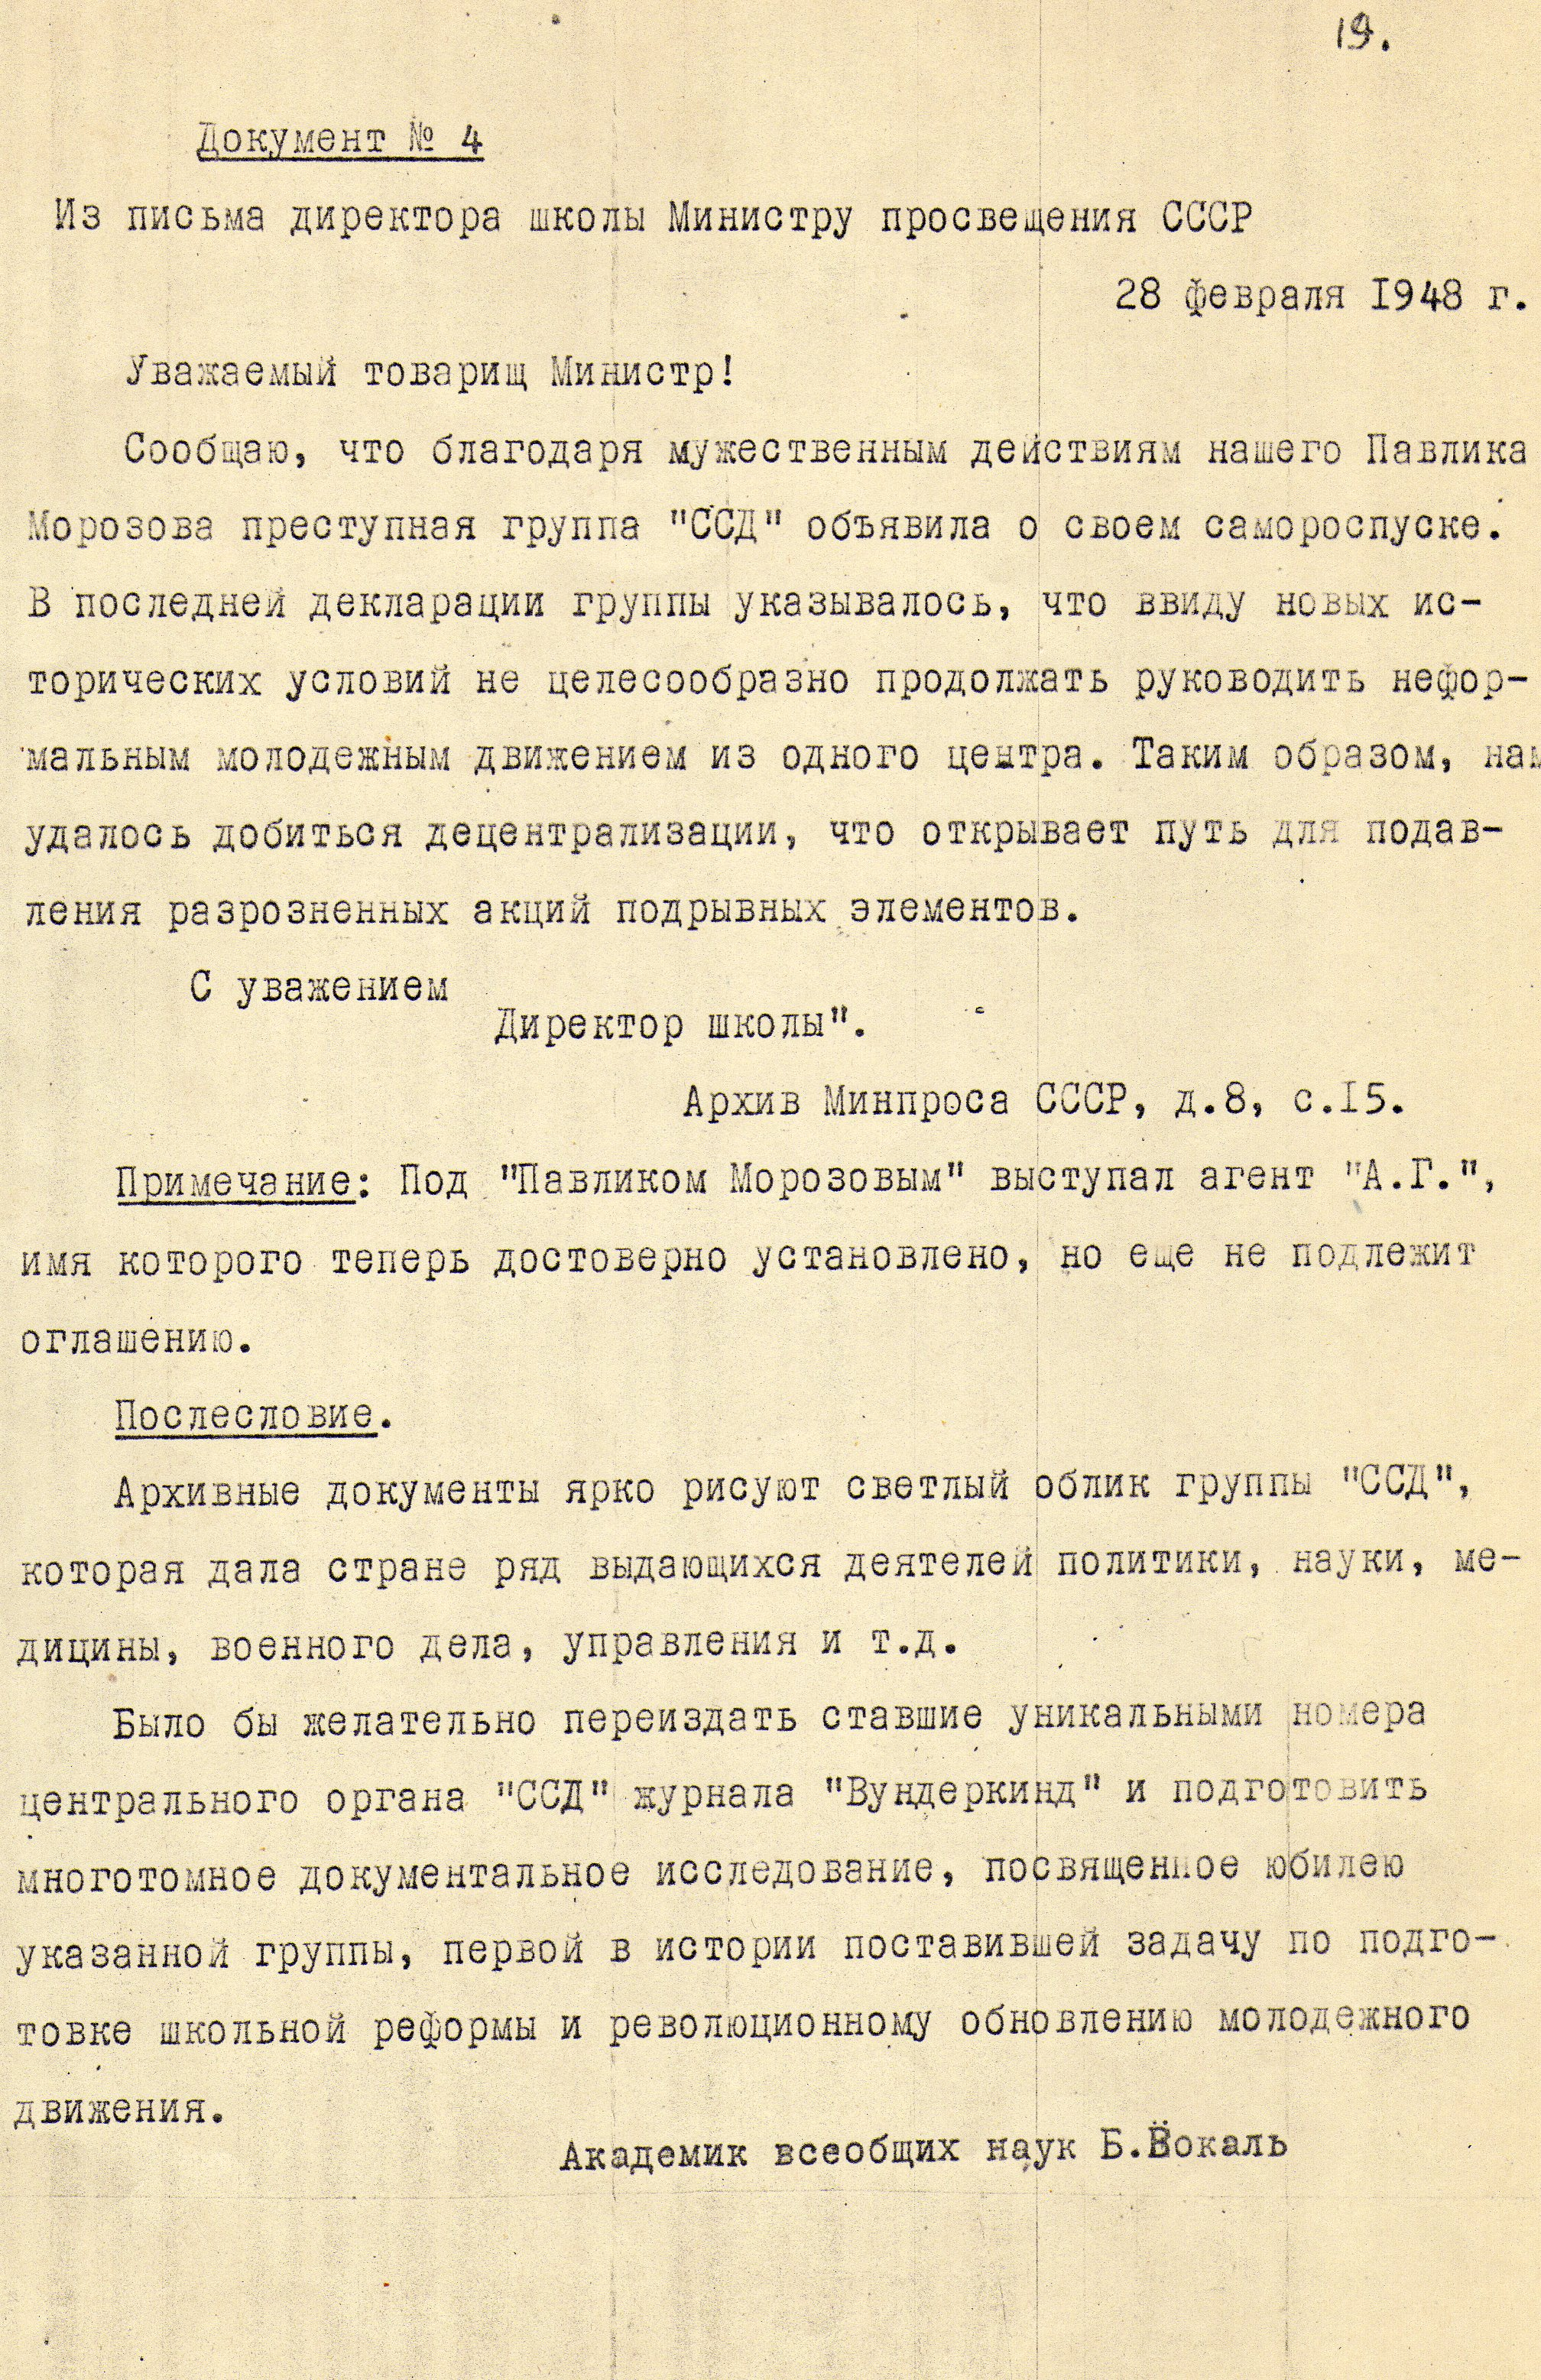
\includegraphics[width=\textwidth]{inc/Vynd/Vynd026}

\noindent
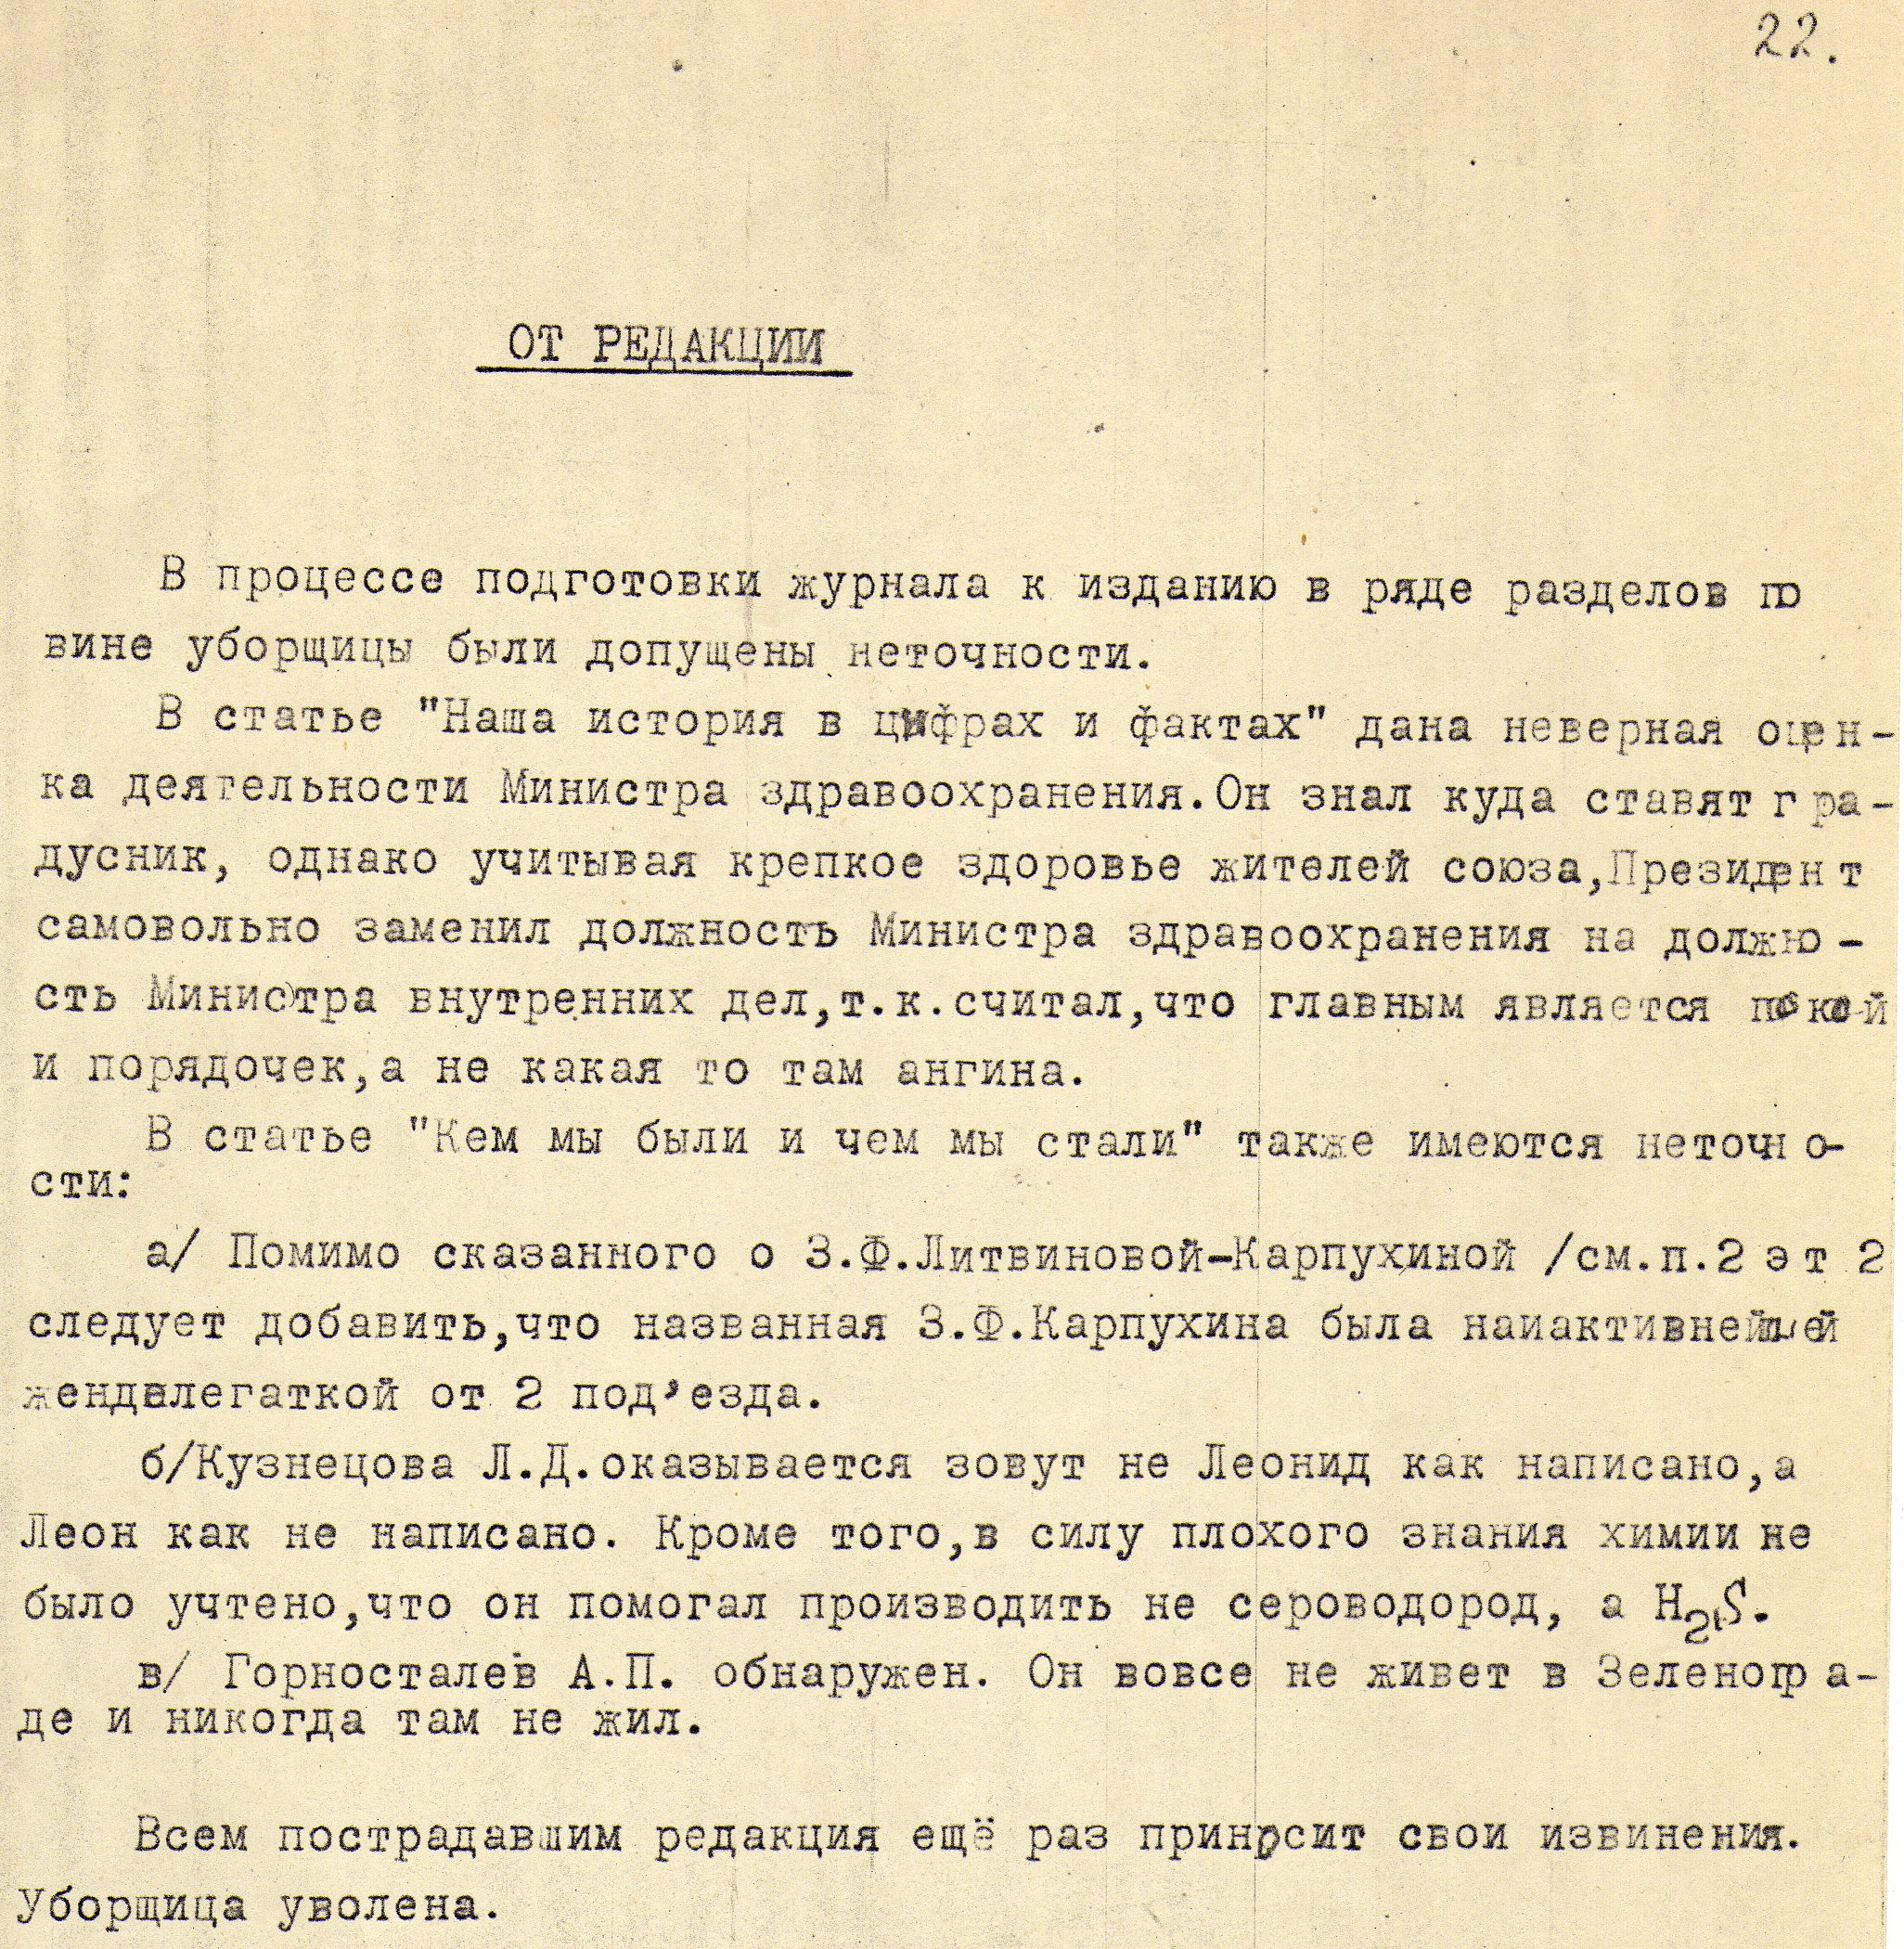
\includegraphics[width=\textwidth]{inc/Vynd/Vynd027}

\noindent
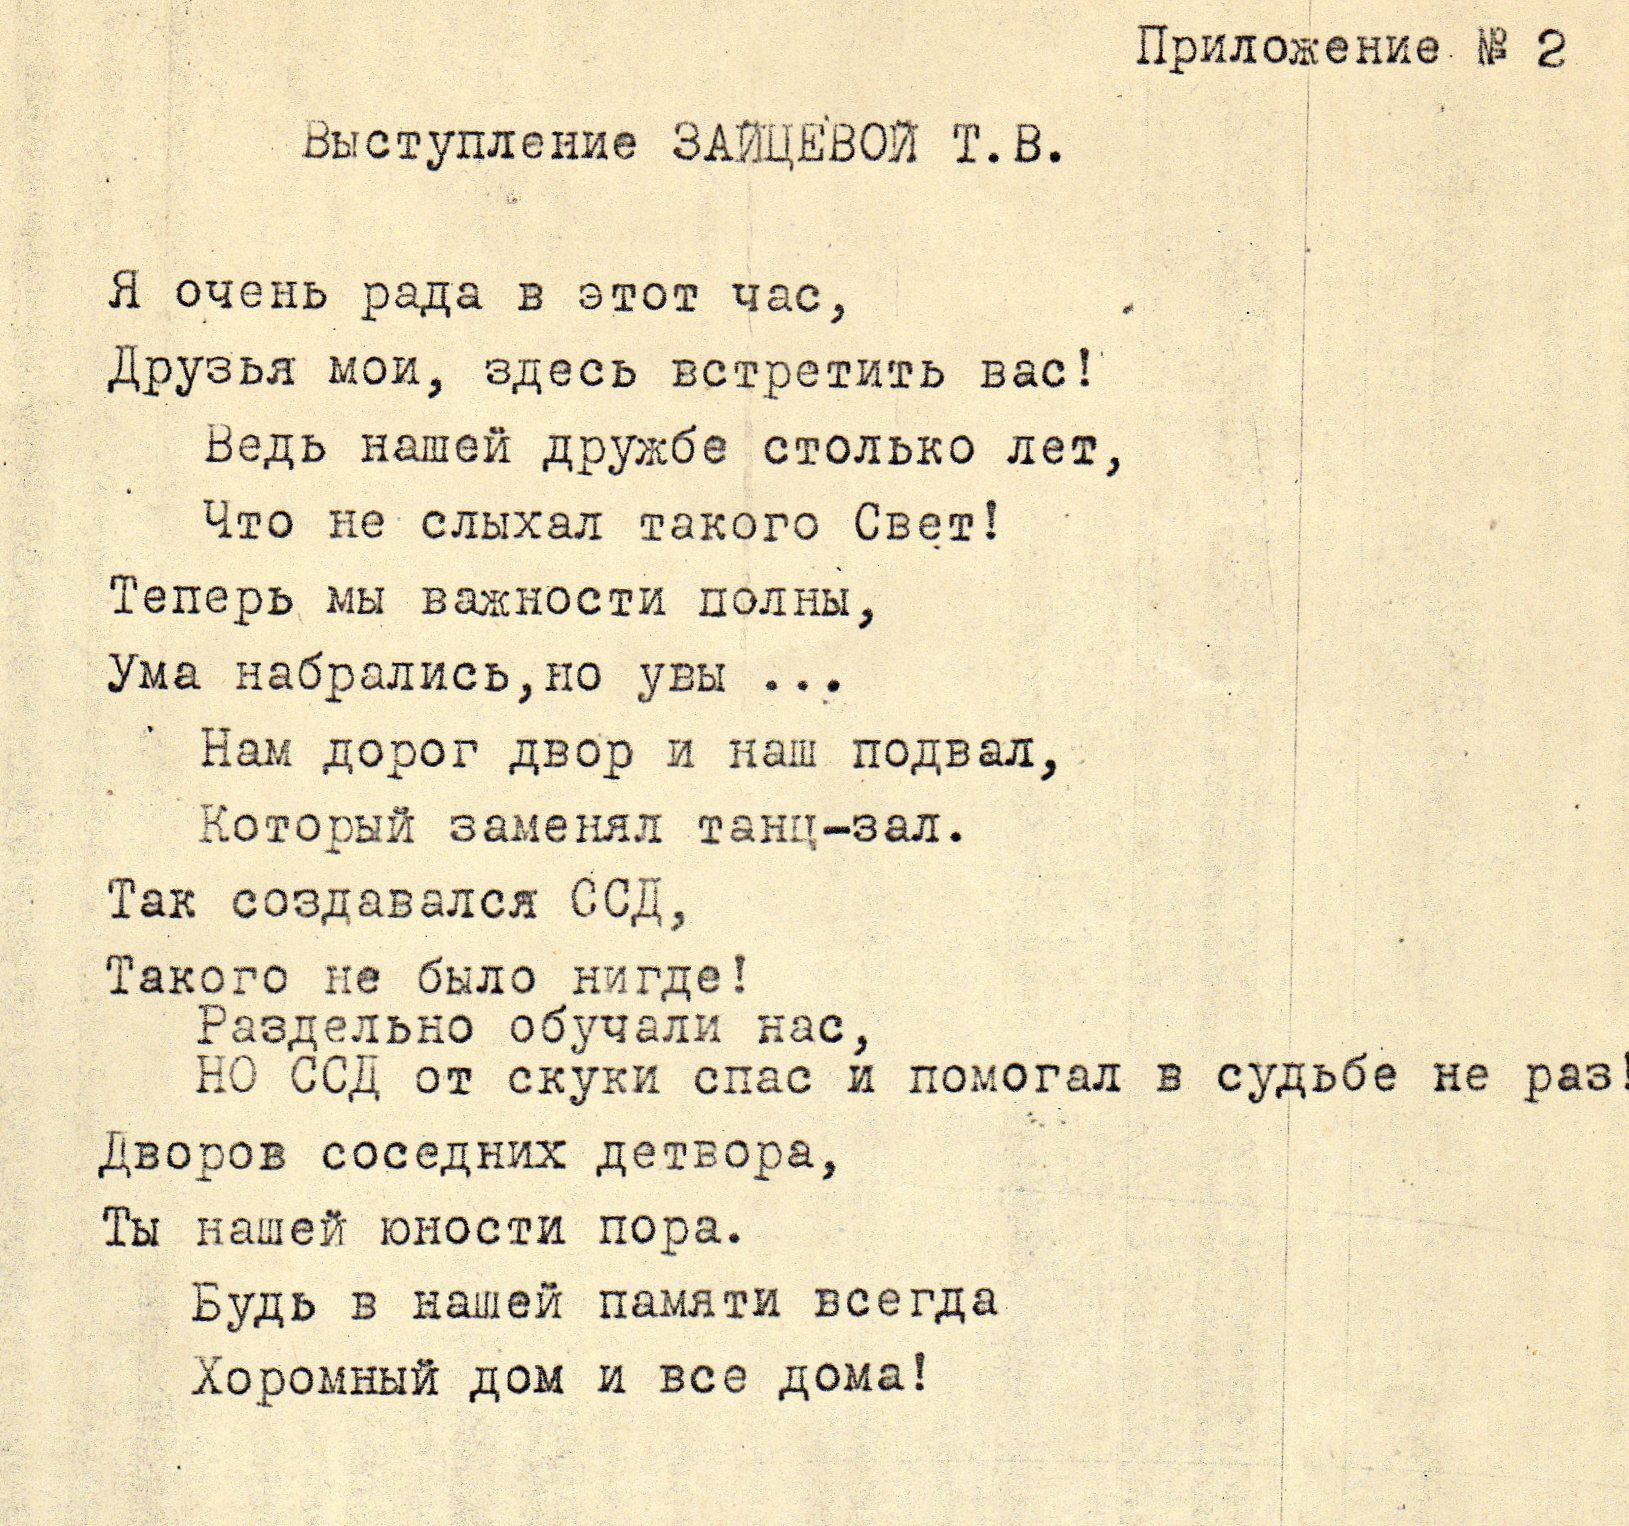
\includegraphics[width=\textwidth]{inc/Vynd/Vynd028}

\restoregeometry

